% ---------------------------------------------------------------
% TCC2 - SENAC SANTO AMARO
% ---------------------------------------------------------------

\documentclass[
    12pt,                % tamanho da fonte
    openright,           % capítulos começam em página ímpar
    oneside,             % para impressão em apenas um lado do papel
    a4paper,             % tamanho do papel
    english,             % idioma adicional
    brazil               % idioma principal
]{abntex2}

% ---------------------------------------------------------------
% PACOTES
% ---------------------------------------------------------------
\usepackage{lmodern}                % Fonte Latin Modern
\usepackage[T1]{fontenc}            % Seleção de códigos de fonte
\usepackage[utf8]{inputenc}         % Codificação do documento
\usepackage{lastpage}               % Usado pela Ficha catalográfica
\usepackage{indentfirst}            % Indenta o primeiro parágrafo
\usepackage{color}                  % Controle de cores
\usepackage{graphicx}               % Inclusão de gráficos
\usepackage{microtype}              % Melhorias de justificação
\usepackage{float}                  % Para posicionamento de figuras
\usepackage{booktabs}               % Tabelas profissionais
\usepackage{multirow}               % Células mescladas em tabelas
\usepackage{longtable}              % Tabelas longas
\usepackage{amsmath,amssymb}        % Símbolos matemáticos
\usepackage{pgfgantt}               % Diagramas de Gantt
\usetikzlibrary{arrows.meta,positioning,fit,calc} % Diagramas do desenvolvimento
\usepackage{pgfplots}                % Gráficos dos resultados
\pgfplotsset{compat=1.18}
\usepgfplotslibrary{groupplots}
\usepackage[brazilian,hyperpageref]{backref}  % Páginas com citações
\usepackage[alf]{abntex2cite}       % Citações ABNT
%Adicionados posteriormente:
\usepackage{tabularx} % Para tabelas com largura ajustada
\usepackage{booktabs} % Para linhas mais elegantes (estilo acadêmico)
\usepackage{siunitx}  % Para alinhar números se desejar
\usepackage[table]{xcolor}
\usepackage{adjustbox}
\usepackage[acronym, automake, nopostdot]{glossaries}
\usepackage{subcaption}
% ---------------------------------------------------------------
% CONFIGURAÇÕES DO PDF
% ---------------------------------------------------------------
\makeatletter
\hypersetup{
    pdftitle={\@title},
    pdfauthor={\@author},
    pdfsubject={TCC2 - SENAC Santo Amaro},
    pdfcreator={LaTeX with abnTeX2},
    pdfkeywords={tcc2}{senac}{santo amaro}{trabalho de conclusão},
    colorlinks=true,        % false: links em caixas; true: links coloridos
    linkcolor=blue,         % cor dos links internos
    citecolor=blue,         % cor dos links para bibliografia
    filecolor=magenta,      % cor dos links para arquivos
    urlcolor=blue,
    bookmarksdepth=4
}
\makeatother

% ---------------------------------------------------------------
% CONFIGURAÇÕES DE APARÊNCIA DO PDF FINAL
% ---------------------------------------------------------------
\definecolor{blue}{RGB}{41,5,195}

% ---------------------------------------------------------------
% TAMANHO DA FONTE DAS LEGENDAS (ABNT) -- 10 pt
% ---------------------------------------------------------------
% O título (\caption) e a linha de fonte (\legend) de figuras e
% tabelas devem ficar em 10 pt (o corpo do texto é 12 pt). Por
% padrão o memoir/abntex2 deixa essas legendas em 12 pt; os comandos
% abaixo reduzem o título e a fonte para 10 pt.
\renewcommand{\ABNTEXfontereduzida}{\fontsize{10}{12}\selectfont}
\captionnamefont{\ABNTEXfontereduzida}   % rótulo "Figura N"/"Tabela N"
\captiontitlefont{\ABNTEXfontereduzida}  % texto do título da legenda
\makeatletter
% Redefine \legend (usado em "Fonte: ...") para sair em 10 pt
% (a definição original do memoir fixa \normalsize = 12 pt).
\renewcommand{\legend}[1]{%
  \M@gettitle{#1}%
  \memlegendinfo{#1}%
  \par
  \begingroup
    \@parboxrestore
    \if@minipage
      \@setminipage
    \fi
    \ABNTEXfontereduzida
    \captiondelim{\mbox{}}%
    \@makecaption{}{\ignorespaces #1}\par
  \endgroup}
\makeatother

% ---------------------------------------------------------------
% INFORMAÇÕES DO DOCUMENTO
% ---------------------------------------------------------------
\titulo{Análise Comparativa de Desempenho e Eficiência Energética entre Processamento de OCR em Borda e em Nuvem aplicado à Smart Metering.}
\autor{Marcelo Fernandes de Oliveira Junior \\ Gustavo Oliveira dos Santos \\ Christian Lima Santana}
\local{São Paulo}
\data{2026}
\orientador{Afonso César Lelis Brandão}

\instituicao{%
  SENAC -- Serviço Nacional de Aprendizagem Comercial
  \par
  Unidade Santo Amaro
  \par
  Curso de Bacharelado em Ciência da Computação
}

\tipotrabalho{Trabalho de Conclusão de Curso II}

\preambulo{Trabalho de Conclusão de Curso II apresentado ao SENAC Santo Amaro como requisito parcial para conclusão do curso de Bacharelado em Ciência da Computação.}

% ---------------------------------------------------------------
% COMPILA O ÍNDICE
% ---------------------------------------------------------------
\makeindex

\makeglossaries
\newglossaryentry{espidf}{
    name=ESP-IDF,
    description={SDK (Software Development Kit) e framework, desenvolvido pela Espressif, otimizado para programação em microcontroladores ESP32}
}

\newglossaryentry{esp32cam}{
    name=ESP32-CAM,
    description={Módulo para acoplamento no microprocessador ESP32, conferindo ao dispositivo a capacidade de capturar imagens}
}

\newglossaryentry{payload}{
    name=payload,
    description={Caracteres enviados no corpo do pacote de rede}
}

\newglossaryentry{retrofitting}{
    name=retrofitting,
    description={Técnica de modernização ou atualização de dispositivos e equipamentos}
}

\newglossaryentry{cloud_computing}{
    name=Cloud Computing,
    description={Método de processamento em nuvem}
}

\newglossaryentry{edge_computing}{
    name=Edge Computing,
    description={Método de processamento local}
}

\newglossaryentry{smart_metering}{
    name=Smart Metering,
    description={Tecnologias para Medição Inteligente}
}
\newacronym{lorawan}{LoRaWan}{Long Range Wide Area Network}
\newacronym{lpwan}{LPWAN}{Low Power Wide Area Network}
\newacronym{sf}{SF}{Spreading Factor}
\newacronym{cr}{CR}{Coding Rate}
\newacronym{ocr}{OCR}{Optical Character Recognition}
\newacronym{lora}{LoRa}{Long Range}
\newacronym{bw}{BW}{Bandwidth}
\newacronym{otaa}{OTAA}{Over the Air Activation}
\newacronym{abp}{ABP}{Activation by Personalization}
\newacronym{iot}{IoT}{Internet of Things}
\newacronym{pdr}{PDR}{Packet Delivery Ratio}
\newacronym{iaas}{IaaS}{Infrastructure as a Service}
\newacronym{saas}{SaaS}{Software as a Service}
\newacronym{ism}{ISM}{Industrial, Scientific and Medical}
\newacronym{lr_fhss}{LR-FHSS}{Long Range Frequency Hopping Spread Spectrum}
\newacronym{css}{CSS}{Chirp Spread Spectrum}
\newacronym{dr}{DR}{Data Rate}
\newacronym{eirp}{EIRP}{Effective Isotropic Radiated Power}
\newacronym{cnn}{CNN}{Convolutional Neural Network}
\newacronym{ia}{IA}{Inteligência Artificial}
\newacronym{rna}{RNA}{Redes Neurais Artificiais}
\newacronym{qat}{QAT}{Quantization-Aware Training}
\newacronym{crnn}{CRNN}{Convolutional Recurrent Neural Network}
\newacronym{ctc}{CTC}{Connectionist Temporal Classification}
\newacronym{rnn}{RNN}{Recurrent Neural Network}
\newacronym{rgb}{RGB}{Red, Green, Blue}
\newacronym{roi}{ROI}{Region of Interest}
% ---------------------------------------------------------------
% INÍCIO DO DOCUMENTO
% ---------------------------------------------------------------
\begin{document}

% Seleciona o idioma do documento
\selectlanguage{brazil}

% Retira espaço extra obsoleto entre as frases
\frenchspacing

% ---------------------------------------------------------------
% ELEMENTOS PRÉ-TEXTUAIS
% ---------------------------------------------------------------
\pretextual

% ---------------------------------------------------------------
% CAPA
% ---------------------------------------------------------------
\imprimircapa

% ---------------------------------------------------------------
% FOLHA DE ROSTO
% ---------------------------------------------------------------
\imprimirfolhaderosto

% ---------------------------------------------------------------
% RESUMO
% ---------------------------------------------------------------
\begin{resumo}
Este trabalho busca propor uma análise comparativa entre dois métodos de processamento
para sistemas de \gls{smart_metering} (medição inteligente): \gls{edge_computing} (Computação em Borda), 
com inferência de \gls{ocr} realizada localmente no microcontrolador \gls{esp32cam} 
por meio de modelo de aprendizado de máquina treinado de forma supervisionada 
e quantizado em inteiros de 8 bits, 
e \gls{cloud_computing} (Computação em Nuvem), com inferência realizada em ambiente 
remoto através de modelo treinado de forma supervisionada e quantizado em ponto flutuante de 32 bits.
A motivação reside no elevado custo de substituição dos mais diversos medidores convencionais, 
amplamente utilizados em ambientes residenciais e privados, 
por modelos inteligentes nativos. O que favorece o \textit{\gls{retrofitting}} 
como alternativa mais economicamente viável. 
A transmissão dos dados entre os nós de borda e o gateway central é realizada via rede \gls{lorawan},
utilizando o Spreading Factor SF8, configuração que assegura conformidade com o limite
regulatório de \textit{dwell time} de 400~ms estabelecido pelo Ato n\textordmasculine~14.448
da ANATEL, ao mesmo tempo em que maximiza o alcance dentro desse limite. A viabilidade
do envio de imagens fragmentadas via \gls{lorawan} foi demonstrada analiticamente, com
uma imagem de 160$\times$120 pixels em escala de cinza, comprimida utilizando o algoritmo JPEG com
aproximadamente 3,10~KB, podendo ser transmitida em 38 pacotes em cerca de 13,3~s
de rádio ativo. Os dois fluxos de processamento
serão avaliados segundo três métricas quantitativas: acurácia de leitura \gls{ocr} (\%),
latência de ponta a ponta (ms), consumo energético por leitura (mAh). 
O objetivo deste trabalho é apresentar resultados orientem a escolha arquitetural
mais adequada para implantações de \textit{Smart Metering} em larga escala, considerando
o \textit{trade-off} entre eficiência energética, precisão de reconhecimento e complexidade
de manutenção do sistema.

\vspace{\onelineskip}

\noindent
\textbf{Palavras-chave}: Smart Metering. ESP32. LoRaWan. OCR.
\end{resumo}


% ---------------------------------------------------------------
% ABSTRACT (RESUMO EM LÍNGUA ESTRANGEIRA) -- OBRIGATÓRIO NO TCC2
% ---------------------------------------------------------------
% Versão em inglês do resumo. Deve conter o mesmo conteúdo do resumo
% em português (problema, objetivo, método, resultados e conclusão)
% e as palavras-chave traduzidas (Keywords). Pela ABNT NBR 14724, o
% resumo em língua estrangeira vem logo após o resumo em português.
\begin{resumo}[Abstract]
 \begin{otherlanguage*}{english}
    This work aims to propose a comparative analysis between two processing methods
    for \gls{smart_metering} systems: \gls{edge_computing}, 
    with OCR inference performed locally on the \gls{esp32cam} microcontroller 
    using a machine learning model trained in a supervised manner 
    and quantized to 8-bit integers, 
    and \gls{cloud_computing}, with inference performed in a remote environment 
    through a model trained in a supervised manner and quantized to 32-bit floating point.
    The motivation lies in the high replacement cost of the most diverse conventional meters, 
    widely used in residential and private environments, 
    by native smart models. This favors \textit{\gls{retrofitting}} 
    as a more economically viable alternative. 
    Data transmission between the edge nodes and the central gateway is carried out via a \gls{lorawan} network,
    using Spreading Factor SF8, a configuration that ensures compliance with the
    dwell time regulatory limit of 400~ms established by ANATEL Act No.~14.448,
    while maximizing range within that limit. The feasibility
    of sending fragmented images via \gls{lorawan} was demonstrated analytically, with
    a 160$\times$120 pixel grayscale image, compressed using the JPEG algorithm to
    approximately 3.10~KB, which can be transmitted in 38 packets in about 13.3~s
    of active radio time. The two processing flows
    will be evaluated according to three quantitative metrics: \gls{ocr} reading accuracy (\%),
    end-to-end latency (ms), energy consumption per reading (mAh). 
    The objective of this work is to present results that guide the most appropriate architectural choice
    for large-scale \textit{Smart Metering} deployments, considering
    the \textit{trade-off} between energy efficiency, recognition precision, and system maintenance complexity.
  \vspace{\onelineskip}
  \noindent
  \textbf{Keywords}: Smart Metering. ESP32. LoRaWan. OCR.
 \end{otherlanguage*}
\end{resumo}

% ---------------------------------------------------------------
% LISTA DE ILUSTRAÇÕES (FIGURAS)
% ---------------------------------------------------------------
% Gerada automaticamente a partir das \caption{} das figuras.
% Toda figura com legenda passa a constar nesta lista.
\pdfbookmark[0]{\listfigurename}{lof}
\listoffigures*
\cleardoublepage

% ---------------------------------------------------------------
% LISTA DE TABELAS
% ---------------------------------------------------------------
% Gerada automaticamente a partir das \caption{} das tabelas.
\pdfbookmark[0]{\listtablename}{lot}
\listoftables*
\cleardoublepage

% ---------------------------------------------------------------
% LISTA DE ABREVIATURAS E SIGLAS
% ---------------------------------------------------------------
\pdfbookmark[0]{Lista de Abreviaturas e Siglas}{siglas}
% \chapter*{Lista de Abreviaturas e Siglas}
\printglossary[type=\acronymtype, title={Lista de Abreviaturas e Siglas}]
\cleardoublepage

\vspace{\onelineskip}

% ---------------------------------------------------------------
% SUMÁRIO
% ---------------------------------------------------------------
\pdfbookmark[0]{\contentsname}{toc}
\tableofcontents*
\cleardoublepage

% ---------------------------------------------------------------
% ELEMENTOS TEXTUAIS
% ---------------------------------------------------------------
\textual

% ===============================================================
% CAPÍTULO 1 - INTRODUÇÃO
% ===============================================================
\chapter{Introdução}
\label{cap:introducao}
Atualmente, a implantação de conceitos de \gls{iot} nos mais diferentes dispositivos presentes 
no dia a dia de milhões de pessoas ao redor do mundo está numa crescente jamais antes vista. 
Como explicado por \citeonline{Tedjojuwono2024}, a adoção de dispositivos \gls{iot} é um dos principais
pilares na ascensão da indústria 4.0, principalmente na pauta da construção de cidades inteligentes. 
E ainda, por característica, tais tecnologias viabilizam a coleta de dados de forma constante, promovendo insumos para realização
de análises, manutenções e aprimoramentos de sistemas através de planos de ação mais eficientes e eficazes. 

Em contrapartida, como explicado por \citeonline{fortune2025} e \citeonline{polimi2020}, 
o alto custo inicial exigido para realizar a transição de dispositivos analógicos para soluções inteligentes nativas
constitui o principal entrave para a adoção de tais tecnologias em larga escala. 
A complexidade de infraestrutura necessária para a substituição física dos medidores limita a viabilidade econômica de projetos 
em áreas privadas de pequeno e médio porte. 

Abordando a pauta de automação residencial e comercial, 
o tema de smart metering surge como ponto focal na discussão. 
Como evidenciado pelo contraste em abordagens de \citeonline{SilvaVilela2021} e \citeonline{adam2022}, 
o desenvolvimento de sistemas focados em smart metering 
enfrenta um impasse arquitetônico, 
onde o método de processamento divergia entre os projetos.

A implementação proposta por \citeonline{SilvaVilela2021} é a denominada \gls{edge_computing}, 
onde o processamento é realizado localmente no dispositivo final, 
assim otimizando recursos energéticos e latência. 
Em oposição, a proposta de \citeonline{adam2022}, realizando processamento em cloud (\gls{cloud_computing}), 
surge como uma solução focada em facilidade de manutenção, 
utilização de softwares mais robustos e menor complexidade de implementação.

Neste contexto, a finalidade deste trabalho é realizar 
a comparação entre os métodos de processamento citados, 
definindo limites, vantagens e desvantagens sob determinado ambiente.


% ---------------------------------------------------------------
\section{Contextualização do problema}
\label{sec:contexto}
O mundo, neste momento, está passando pelo que pode ser chamado como a era da digitalização, 
havendo severas transformações no modo de transmissão de dados e informações \cite{Tedjojuwono2024}. 
Atualmente, a humanidade encontra-se sob influência da expansão da denominada indústria 4.0,
que tem como foco a digitalização dos processos de manufatura e produção, mas que engloba 
inclusive o modo de vida e acesso à informações da sociedade sob o braço 
tecnológico denominado \textit{Cidades Inteligentes}.

Neste contexto, a utilização de hardware inteligente deixou de ser mero luxo de grandes
corporações para se tornar o paradigma central na mudança citada anteriormente. Em relação à equipamentos de medição inteligentes,
também classificados como \gls{smart_metering}, hoje já há uma série de avanços que possibilitam o processamento 
de dados de maneira mais veloz e eficiente. Mas essa evolução também acompanhou a necessidade de adaptação de infraestrutura, 
assim agregando altos custos para à transição das tecnologias analógicas para o digital \cite{Stefano2019}.

Como apresentado por \citeonline{Stefano2019}, o \gls{retrofitting} é uma das soluções mais difundidas para contornar o 
alto custo de digitalização de sistemas nativamente analógicos. Tal conceito, tem como objetivo realizar a digitalização 
de sistemas analógicos reaproveitando o hardware já existente. Essa concepção, é amplamente abordada na academia, havendo grandes teses,
trabalhos e dissertações sobre o tema.

Diante de tal abordagem para redução de custos, a aplicabilidade da técnica de \gls{retrofitting} enfrenta um impasse.
Atualmente, na academia encontra-se mais difundido trabalhos que abordam o uso de microcontroladores aliados à tecnologia \gls{lora}
utilizando o método de processamento em borda, como explicado por \citeonline{SilvaVilela2021}, a utilização deste método 
traz grandes vantagens em relação à latência e otimização de consumo energético. Em oposição, como \citeonline{andriulo2024edge} apresenta, 
o método de processamento em cloud destaca-se por proporcionar maior granularidade de dados, simplificação no desenvolvimento 
de firmware e acurácia ligeiramente melhor em relação ao conceito de \gls{edge_computing}. Todavia, permanece a dúvida de qual 
método de processamento utilizar no desenvolvimento de uma solução \gls{iot} baseado na técnica de \gls{retrofitting}. 
A resolução do problema criará um alicerce, auxiliando o desenvolvimento de futuras ferramentas, que por concepção, apresentará a 
mesma natureza de problemática.


% ---------------------------------------------------------------
\section{Formulação do problema}
\label{sec:problema}
Com base no contexto apresentado, 
revela-se a dúvida sobre os impactos arquitetônicos 
causados pela escolha de métodos de processamento em determinado projeto. 
Este trabalho busca responder o questionamento: 
De que maneira a adoção de determinado método de processamento, 
em borda ou em nuvem, impacta a eficiência energética, acurácia, 
complexidade de desenvolvimento de firmware e desempenho 
computacional de um sistema IOT voltado 
para coleta de dados de medidores analógicos?

% ---------------------------------------------------------------
\section{Objetivos e hipótese}
\subsection{Objetivo geral}

Comparar a viabilidade técnica, a acurácia e o consumo energético entre o processamento de \gls{ocr} realizado localmente no \gls{esp32cam} (abordagem Edge Computing) e a inferência \gls{ocr} realizada remotamente em servidor na nuvem (Cloud), utilizando a rede \gls{lorawan} como meio de transmissão.

\subsection{Objetivos específicos}

\begin{enumerate}
    \item Implementar os dois fluxos de processamento que compõem o experimento comparativo: o fluxo Edge, em que o \gls{ocr} ocorre localmente no \gls{esp32cam}; e o fluxo Cloud, em que a imagem é transmitida para processamento remoto; % 1. construção do experimento
    \item Configurar a rede \gls{lorawan} conectando os nós da rede com o objetivo de reduzir ao máximo o consumo energético; % 2. Configuração da infrastrutura de rede
    \item Avaliar e comparar os dois fluxos segundo as métricas: precisão de leitura (\%), latência de processamento (ms), consumo energético por leitura (mAh) e volume de dados transmitidos (bytes/leitura), identificando o \textit{trade-off} entre processamento local e transmissão. % 3. Responde a pergunta central do TCC
\end{enumerate}

\subsection{Hipótese}
\label{subsec:hipotese}
Considerando o trade-off apresentado, 
foram estabelecidas hipóteses com o objetivo de verificar 
se a utilização de determinada abordagem apresenta vantagens 
quando observadas sob o mesmo cenário.
As hipóteses orientam a definição dos experimentos e a 
análise dos resultados obtidos.

\begin{itemize}
	\item \textbf{H1}: A quantização em inteiros de 8 bits, aplicada ao modelo implementado no fluxo de processamento em borda, causa redução de acurácia em comparação ao modelo quantizado em ponto flutuante de 32 bits, implementado no fluxo de processamento em nuvem.
    \item \textbf{H2}: O método de processamento local apresenta custo computacional maior, no dispositivo final, em comparação com o método de processamento remoto.
    \item \textbf{H3}: A abordagem de processamento em nuvem apresenta autonomia energética inferior durante a transmissão de mensagens quando comparada ao método de processamento local.
\end{itemize} 

% ---------------------------------------------------------------
\section{Justificativa}
\label{sec:justificativa}
Este trabalho propõe uma abordagem analítica sobre métodos de processamento 
implementados em sistemas baseados em tecnologias \gls{iot} com o objetivo 
de aplicação da técnica de \gls{retrofitting} em instrumentos de medição analógicos.
Tal temática tem como alicerce a lacuna literária identificada por \citeonline{andriulo2024edge}, 
na qual carecem trabalhos que apresentam informações úteis para a etapa de desenvolvimento arquitetural 
de tais ferramentas.

Diante de tal contexto, revela-se a importância acadêmica deste trabalho, 
apresentando de forma científica comparações entre os métodos de processamento, 
definindo limites e estipulando vantagens na adoção de determinado método. E ainda, 
este trabalho tem como pauta discorrer sobre os temas: 
desenvolvimento de sistemas baseados em tecnologia \gls{lora},
aplicação de algoritmos de packet loss (perda de pacotes) e
uplink de dados segmentados em pacotes via \gls{lorawan}.

O desenvolvimento deste trabalho tem por foco a disponibilização de insumos para 
tomada de decisões no desenvolvimento de sistemas \gls{iot} que empregam protocolos de 
rede de baixa largura de banda.

% ===============================================================
% CAPÍTULO 2 - REVISÃO BIBLIOGRÁFICA
% ===============================================================
\chapter{Revisão bibliográfica}
\label{cap:revisao}

% ---------------------------------------------------------------
\section{Metodologia da pesquisa bibliográfica}
\label{sec:metodologia_pesquisa_bib}
A pesquisa bibliográfica foi conduzida de forma sistemática, 
estruturando-se em três temas principais: Hardware, Software e Redes. 
Para a seleção dos trabalhos, utilizaram-se as bases de dados Google Scholar, MDPI e Intechopen.

O processo de seleção seguiu um fluxo de filtragem (funil). 
Inicialmente, foram identificados 120 artigos por meio da análise de títulos, 
utilizando strings de busca majoritariamente em inglês, 
tais como ``iot AND energy efficiency'' e ``ESP32 AND camera monitoring''. 
Como ferramentas auxiliares na descoberta de conexões entre autores e na triagem inicial de relevância, 
foram utilizadas as plataformas ResearchRabbit e Gemini Deep Research.

Na etapa de refinamento, aplicou-se a leitura dos resumos (abstracts) 
e a verificação de disponibilidade integral dos textos. 
Foram adotados como critérios de inclusão: artigos publicados entre 2020 e 2026, 
relevância direta para sistemas de telemetria e foco em implementações práticas. 
Como critério de exclusão, descartaram-se trabalhos com acesso restrito ou que não 
apresentassem detalhes técnicos sobre a integração dos eixos propostos.

\begin{table}[H]
    \centering
    \caption{Strings de busca utilizadas no levantamento bibliográfico.}
    \label{tab:strings_busca}
    \begin{tabular}{@{}lll@{}}
    \toprule
    \textbf{ID} & \textbf{Eixo Temático} & \textbf{String de Busca} \\ \midrule
        ST01 & Redes & "IoT" AND "\gls{lorawan}" AND "water waste" \\
        ST02 & Contexto & smart water meter market \\
        ST03 & Contexto & smart water meter costs and benefits \\
        ST04 & Hardware & "IoT" AND "energy efficiency" \\
        ST05 & Hardware & "ESP32" AND "camera monitoring" \\
        ST06 & Hardware & "\gls{esp32cam}" AND "analog meter" AND "OCR" \\
        ST08 & Software & "automatic meter reading" OCR accuracy "error rate" evaluation \\
        ST09 & Redes & "packet delivery ratio" \gls{lorawan} "latency" monitoring system \\
        ST010 & Contexto & "water consumption prediction" "mean absolute error" forecasting metrics \\ \bottomrule
    \end{tabular}
\end{table}

% ---------------------------------------------------------------
\section{Fundamentos teóricos}
\label{sec:fundamentos}
\subsection{LoRa}
Como explicado por \citeonline{Camargo2022}, \gls{lora} é uma tecnologia, patenteada e desenvolvida pela Semtech, que tem como foco viabilizar a transmissão de dados sem fio em longo alcance através de radiofrequência.

A rede \gls{lorawan} é constituída por dispositivos finais, gateways e servidores de rede/aplicação.
Com o objetivo de realizar um gerenciamento mais fino de consumo energético, a comunicação entre os dispositivos finais e servidores de rede é definida por três classes como demonstrado na tabela~\ref{tab:tabela_classes}.

\begin{table}[H]
    \centering
    \caption{Classes de Configuração LoRa}
    \label{tab:tabela_classes}
    \begin{tabular}{|l|p{6cm}|p{6cm}|}
        \toprule
        \textbf{Classe} & \textbf{Descrição} & \textbf{Característica} \\
        \midrule
        Classe A & O dispositivo final é habilitado a receber downlink imediatamente após ser realizado um envio de mensagem (uplink). & Menor consumo energético e menor tráfego de mensagens. \\
        \midrule
        Classe B & O dispositivo final é habilitado a receber downlink em períodos agendados e conhecidos. & Consumo energético significativamente maior que a classe A, mas viabiliza comunicação mais frequente entre servidor e dispositivo final. \\
        \midrule
        Classe C & O dispositivo final é continuamente habilitado a receber downlink. & Consumo energético muito alto, mas viabiliza a comunicação entre as partes de forma quase ininterrupta.  \\
        \bottomrule
    \end{tabular}
    \begin{quote}
        Fonte: Adaptado de Semtech Corporation \cite{semtech2024an1200_87}.
    \end{quote}
\end{table}

\begin{figure}[H]
    \centering
    \caption{Campos contidos em um pacote de Uplink}
    \label{fig:lora_uplink}
    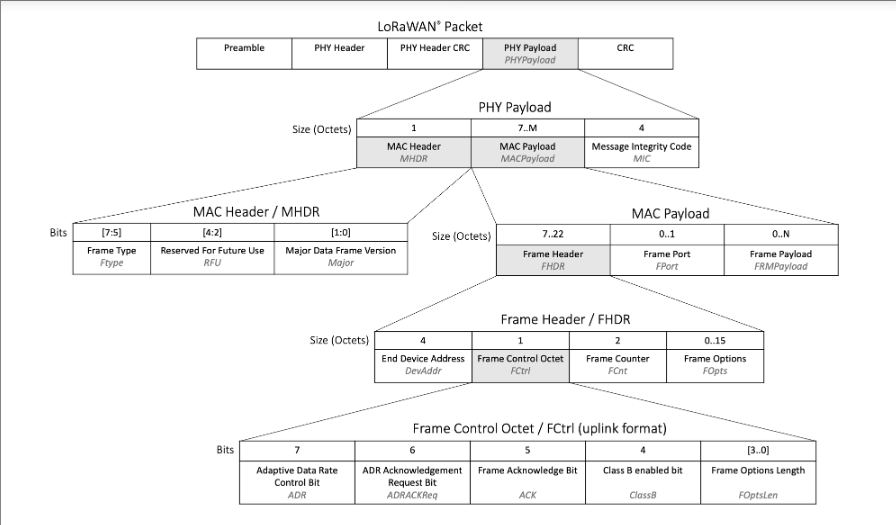
\includegraphics[width=0.85\textwidth]{sections/imagens/SemTech_Uplink_Dataframe.png}
    \small
    \begin{quote}
        Fonte: Adaptado de Semtech Corporation \cite{semtech2024an1200}.
    \end{quote}
\end{figure}

A figura~\ref{fig:lora_uplink} apresenta a estrutura de pacote de rede que é utilizada na tecnologia LoRa. 
Tal estrutura é utilizada tanto no envio de dados pelo dispositivo final (uplink) quanto no recebimento de dados (downlink).

\begin{figure}[H]
    \centering
    \caption{Campos contidos em Frame Header em Downlink}
    \label{fig:fhdr_lora_downlink}
    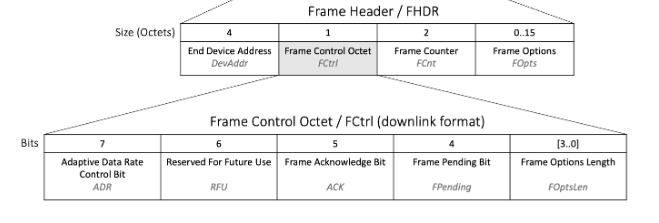
\includegraphics[width=0.85\textwidth]{sections/imagens/SemTech_Downlink_Dataframe.png}
    \small
    \begin{quote}
        Fonte: Adaptado de Semtech Corporation \cite{semtech2024an1200}.
    \end{quote}
\end{figure}

A estrutura do pacote de rede de uplink e downlink é a mesma, mas há diferenças em flags específicas entre os tipos de transmissão de dados. 
A figura~\ref{fig:fhdr_lora_downlink} apresenta a estrutura do ``Frame Header / FHDR'' utilizada em downlink. As estruturas de pacote divergem na flag de classe B, no uplink, por meio da qual o dispositivo final informa ao servidor estar no modo de recebimento de mensagens em tempo programado, e, no pacote downlink, na flag FPending, utilizada para informar a existência de mais mensagens a serem enviadas pelo servidor/gateway.

Conforme apresentado pela \citeonline{lora_alliance_rp002_105} o tamanho máximo de MACPayload, respeitando o padrão regulatório AU915, que será mais bem explicado e abordado posteriormente, em bytes, é variável e dependente do tamanho ocupado pelo atributo Fopts, que é utilizado para solicitar alterações de parâmetros de rede ao dispositivo final.
Não utilizando repetidores de sinal que interligam dispositivos finais com gateways, o tamanho máximo de MACPayload é de 250 bytes, restando em torno de 227 bytes utilizáveis em \gls{payload}.

Para viabilizar a modulação LoRa em dispositivo final, é necessário realizar a configuração de três parâmetros fundamentais. 
A tabela~\ref{tab:parametros_lora} apresenta as definições dos principais parâmetros que ajustam o funcionamento da rede \gls{lorawan}.

\begin{table}[H]
    \centering
    \caption{Parâmetros de Configuração LoRa}
    \label{tab:parametros_lora}
    \begin{tabular}{|l|p{6cm}|}
        \toprule
        \textbf{Parâmetro} & \textbf{Definição} \\
        \midrule
        
        \gls{bw} & Determina a capacidade máxima de transmissão em determinado período de tempo (medido em kHz).\\
        \midrule
        
        \gls{sf} & Determina o alcance do sinal de rádio; o SF é determinado por classes, nas quais, quanto maior a classe, maior a área de alcance do sinal.\\
        \midrule
        
        \gls{cr} & Número de bits destinados à redundância de dados, utilizado para possibilitar recuperação da mensagem em caso de erros na transmissão.\\
        \bottomrule
    \end{tabular}
    \begin{quote}
        Fonte: Adaptado de \citeonline{Camargo2022}.
    \end{quote}
\end{table}

\subsection{LoRaWan}
O \gls{lorawan} é um protocolo de comunicação baseado na tecnologia \gls{lpwan}, que possui o objetivo de viabilizar a comunicação em grandes distâncias, conciliada ao baixo consumo energético.
O protocolo é open-source e mantido pela LoRa Alliance. 
Como citado anteriormente, a rede \gls{lorawan} é formada por dispositivos finais, gateways, servidores de rede e servidores de aplicação \cite{Camargo2022}. 

A figura~\ref{fig:stack_layer_lora} apresenta a pilha de elementos das camadas MAC e Física que compõem a arquitetura do protocolo \gls{lorawan}.

\begin{figure}[H]
    \centering
    \caption{Pilha de elementos das camadas LoRa/LoRaWan}
    \label{fig:stack_layer_lora}
    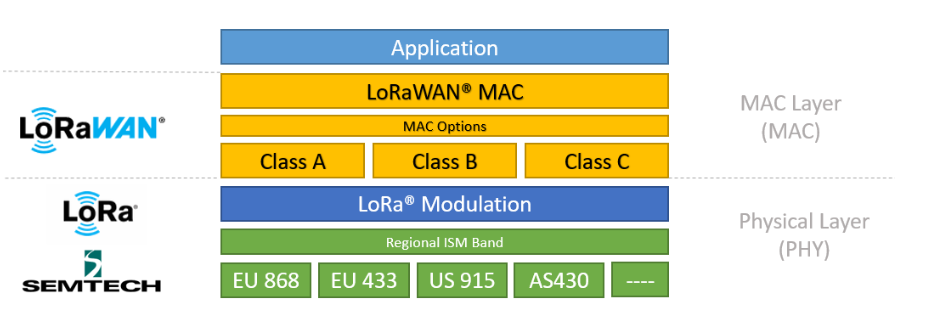
\includegraphics[width=0.85\textwidth]{sections/imagens/LoRaWan_Pilha_Camadas.png}
    \small
    \begin{quote}
        Fonte: Adaptado de Semtech Corporation \cite{semtech2024an1200_86}.
    \end{quote}
\end{figure}

\begin{figure}[H]
    \centering
    \caption{Implementação Típica de Rede LoRaWan}
    \label{fig:implementacao_tipica_lorawan}
    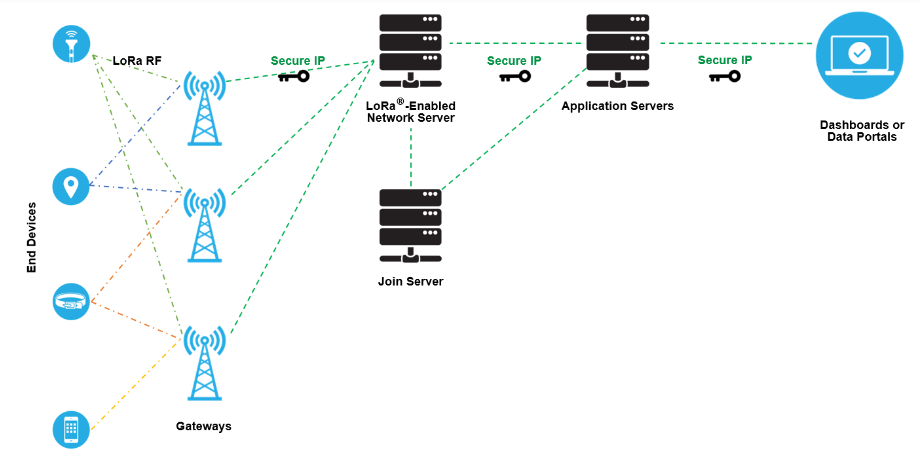
\includegraphics[width=0.85\textwidth]{sections/imagens/Implementacao_tipica_LoRaWan.png}
    \small
    \begin{quote}
        Fonte: Adaptado de Semtech Corporation \cite{semtech2024an1200_86}.
    \end{quote}
\end{figure}

A figura~\ref{fig:implementacao_tipica_lorawan} apresenta a arquitetura típica de um sistema \gls{iot} que utiliza como base o protocolo \gls{lorawan} para viabilizar a comunicação entre os dispositivos. Cada elemento que compõe uma rede \gls{lorawan} possui uma responsabilidade; neste momento, é extremamente válido analisá-las individualmente:

\subsubsection{Dispositivos Finais (End Nodes)}

\citeonline{semtech2024an1200_86} define que dispositivos finais habilitados para LoRaWan são sensores ou atuadores que são conectados a gateways via modulação de radiofrequência LoRa. 

Na maioria das aplicações, esses dispositivos são autônomos, dependentes de baterias como fonte energética primária e possuem como responsabilidade digitalizar condições físicas como temperatura, captura de imagens, níveis de tremulação, entre outros.

Em relação às possíveis configurações que podem ser aplicadas nos dispositivos finais, como apresentado por \citeonline{Camargo2022}, cada nó pode assumir uma das configurações que a tabela~\ref{tab:tabela_classes} apresenta. Outro parâmetro configurável é o tipo de autenticação dos dispositivos em rede, havendo o padrão \gls{otaa}, no qual o próprio dispositivo gerencia a conexão à rede, e a \gls{abp}, na qual os dispositivos são vinculados de forma manual a uma rede em específico, não passando pelo processo de entrada implementado no \gls{otaa}.

O LoRaWan utiliza o padrão AES de criptografia simétrica, aplicado tanto na camada de aplicação quanto na camada de rede.

Os dispositivos finais, corriqueiramente, são desenvolvidos sobre microprocessadores, podendo tanto utilizar placas que já incluem módulos LoRaWan nativos quanto serem desenvolvidos sobre plataformas como ESP32, Arduino, Raspberry Pi, entre outras.
A partir da construção do dispositivo, ou acoplamento de módulos, possibilita-se a captura de dados em ambiente \cite{Camargo2022}.

Como destacado por \citeonline{Sari2022} e \citeonline{Ahmad2021}, o ESP32 destaca-se nesse cenário como uma plataforma robusta de baixo custo, integrando conectividade sem fio e múltiplos modos de operação. 
Diferentemente de arquiteturas mais simples, o ESP32 permite a execução de tarefas complexas e segurança criptográfica sem comprometer severamente o ciclo de vida da bateria, desde que devidamente configurado.

Segundo \citeonline{Ferreira2020}, a vida útil da bateria é influenciada criticamente não apenas pelo hardware, mas pela eficiência das rotinas de escrita em periféricos e pela otimização do firmware.
Diante de tal afirmação, destaca-se a função \textit{deep sleep} presente no ESP32 que possui como foco a minimização do consumo energético quando em estado ocioso.

\begin{figure}[H]
    \centering
    \caption{Módulo ESP32-CAM integrado com LoRa}
    \label{fig:esp32cam_lora}
    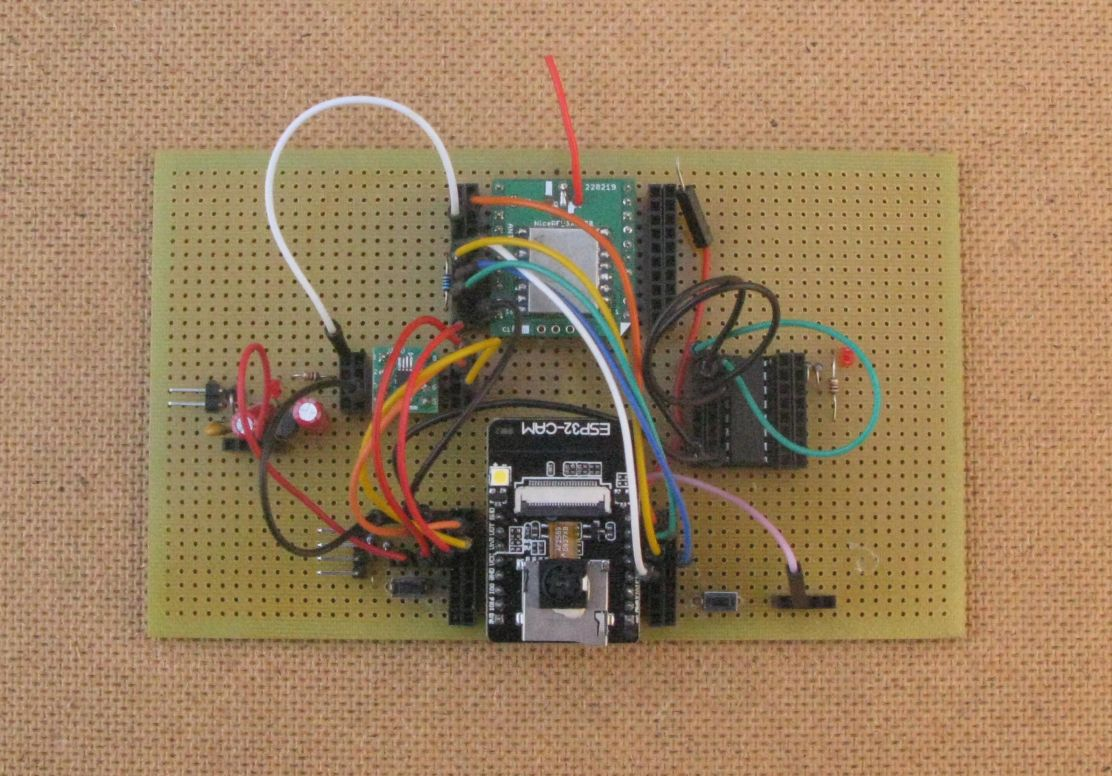
\includegraphics[width=0.85\textwidth]{sections/imagens/ESP32CAM_LoRa.jpg}
    \small
    \begin{quote}
        \centering
        Fonte: \cite{robinson2021stuartcam}.
    \end{quote}
\end{figure}

\subsubsection{Gateways}

O gateway, como demonstrado na figura~\ref{fig:implementacao_tipica_lorawan}, 
é um elemento da rede LoRaWan que tem como responsabilidade agrupar dispositivos finais 
e viabilizar a comunicação entre o dispositivo final e o servidor de rede \cite{Camargo2022}. 

A comunicação entre o dispositivo final e o gateway é realizada via protocolo LoRaWan, 
na qual o gateway pode realizar a tarefa de registrar tráfego de mensagens. 
Como explicado por \citeonline{semtech2024an1200_86}, 
os dispositivos finais, ao realizar o envio de uplink, 
distribuem as suas mensagens a todos os gateways alcançáveis dentro da mesma rede; 
tal função tem como objetivo garantir que ao menos um dos gateways da rede receba e transmita a mensagem ao servidor de rede.

Os gateways operam na camada física e, convencionalmente, 
assumem a responsabilidade apenas de viabilizar o tráfego de requisições uplink e 
downlink e realizar a verificação de integridade do pacote, 
não realizando processamento intermediário da mensagem para 
enviá-la ao servidor de rede \cite{semtech2024an1200_86}.

A comunicação entre o gateway e o servidor de rede, 
corriqueiramente, é estabelecida utilizando protocolo TCP/IP. 
Toda comunicação dentro do protocolo LoRaWan é bidirecional \cite{Camargo2022}.

É possível encontrar gateways prontos de múltiplos canais sendo comercializados, 
mas é plenamente viável desenvolver gateways a partir de módulos e placas 
de prototipagem como a apresentada na figura~\ref{fig:esp32cam_lora}. 

\begin{figure}[H]
    \centering
    \caption{Gateway LoRaWan compatível com placas Raspberry Pi}
    \label{fig:lora_uplink}
    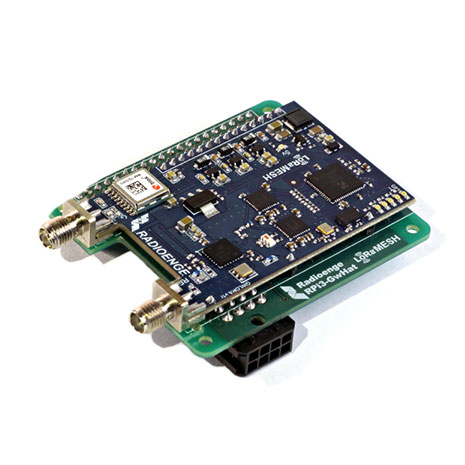
\includegraphics[width=0.85\textwidth]{sections/imagens/gateway-lorawan-radioenge.jpg}
    \small
    \begin{quote}
        \centering
        Fonte: Catálogo de Produtos \cite{radioenge_gateway_lorawan}.
    \end{quote}
\end{figure}


\subsubsection{Servidores de Rede e Aplicação}

Como apresentado por \citeonline{Camargo2022}, 
servidores de rede e servidores de aplicação, 
dada a estrutura em que foram desenvolvidos, 
tanto podem ser implementados sob o mesmo hardware,
como podem estar fisicamente distantes,
realizando comunicação através de protocolo TCP/IP.

Como explicado pela \citeonline{semtech2024an1200_86}, servidores de rede são responsáveis por 
gerenciar dinamicamente a rede de dispositivos, adaptando o sistema para se ajustar a um cenário
de constante mudança de parâmetros. Entre as responsabilidades dos servidores de rede estão: 
receber, descartar duplicatas e descriptografar mensagens enviadas por uplink, 
realizar autenticação, garantir segurança com o protocolo AES,
confirmar recebimento de mensagens, responder a requisições de camada MAC, realizar configuração de 
dispositivos finais através de requisições downlink, entre outras. 

Servidores de Aplicação, por sua vez, são responsáveis por receber 
pacotes enviados pelo servidor de rede, tratar e disponibilizar
em formato de informação ao usuário os dados 
extraídos pelos dispositivos finais. Como a \citeonline{semtech2024an1200_86} explica,
é uma de suas responsabilidades também gerenciar os \gls{payload}s de 
downlink a serem enviados aos dispositivos finais.

Ambos os tipos de servidores possuem diversas soluções
prontas para implementação tanto em ambiente local quanto em nuvem.
Para servidores de rede, destaca-se o Chirp Stack, 
que tem por foco o gerenciamento de dispositivos de \gls{iot} em rede privada.
Já para servidores de aplicação, o Tago IO mostra-se como uma ferramenta robusta,
com foco corporativo e ampla gama de ferramentas 
voltadas para gerenciamento de dispositivos \cite{Camargo2022}.


\subsection{Edge Computing e Cloud Computing}
\begin{figure}[H]
    \centering
    \caption{Distribuição de Trabalhos Relacionados à Computação em IoT}
    \label{fig:dist_trab_rel_comp_iot}
  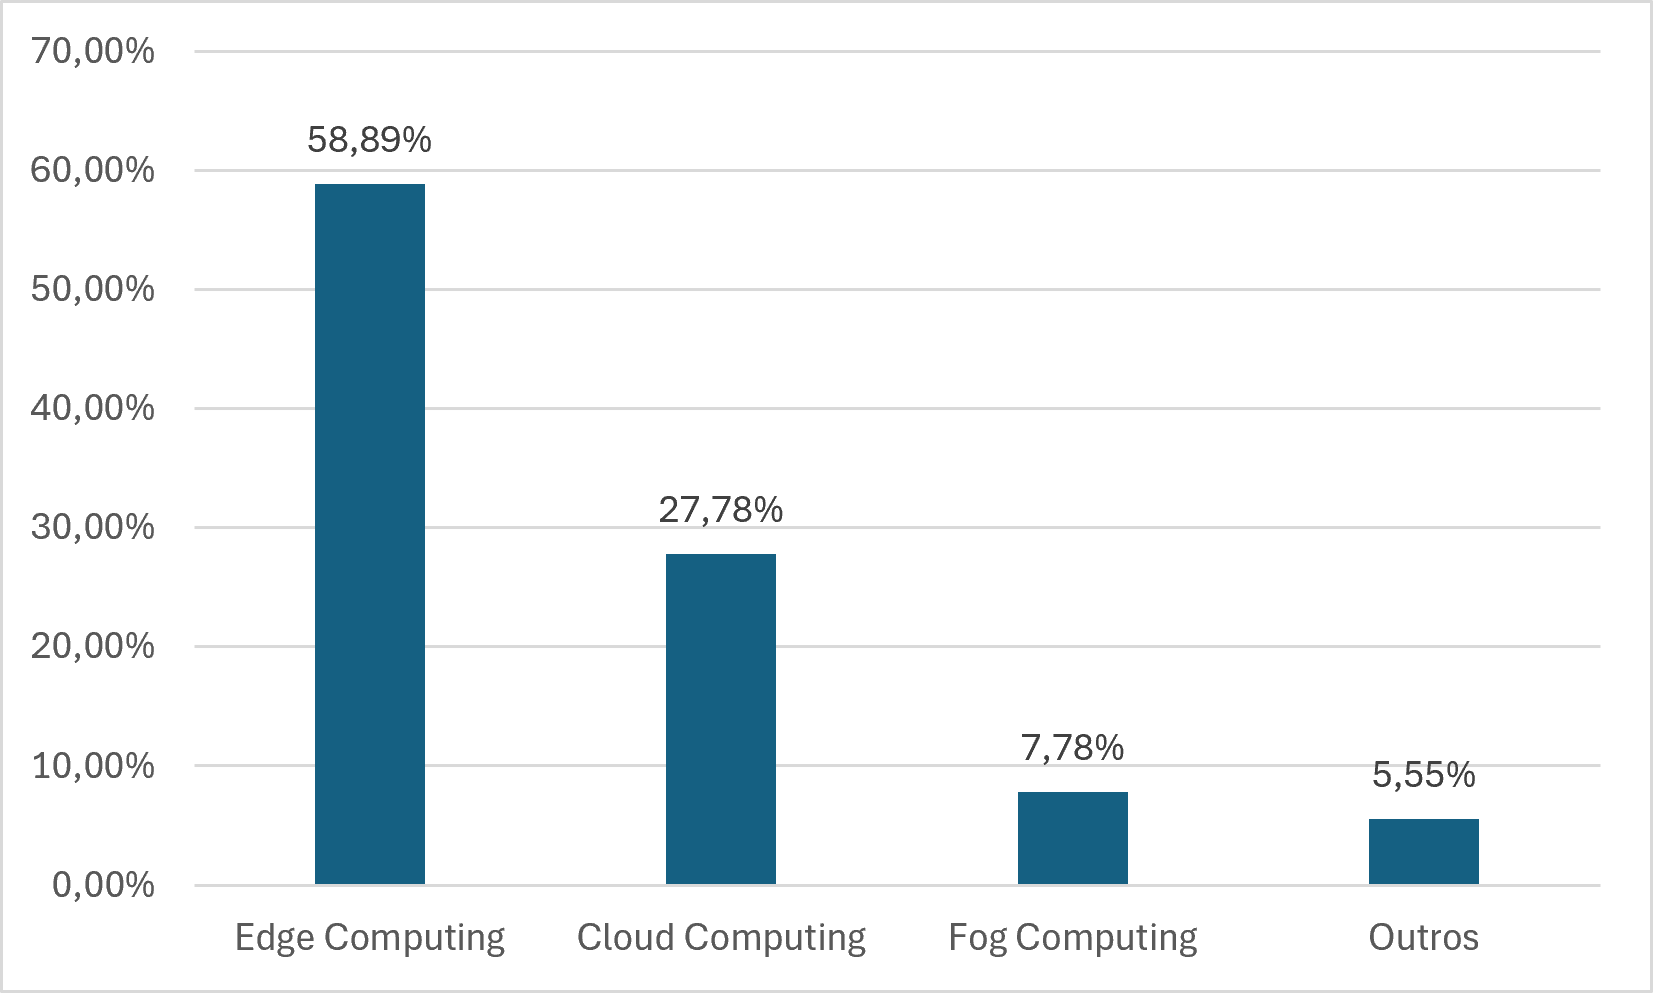
\includegraphics[width=0.85\textwidth]{sections/imagens/trabalhos_relacionados_cloud_edge_computing.png}
    \small
    \begin{quote}
        \centering
        Fonte: Adaptado de \citeonline{andriulo2024edge}.
    \end{quote}
\end{figure}

\gls{edge_computing} (computação em borda), 
em \gls{iot}, é uma arquitetura baseada em processamento descentralizado de dados,
na qual ocorre o processamento com o objetivo de construção de informações a 
partir de dispositivos que têm por responsabilidade inicial a 
extração de dados do ambiente real. Como explicado por \citeonline{andriulo2024edge}, 
o gráfico apresentado na figura~\ref{fig:dist_trab_rel_comp_iot} demonstra que 
\gls{edge_computing} é a abordagem mais amplamente difundida na literatura, 
sendo uma solução voltada à segurança de informações e à otimização de redes 
de baixa largura de banda, promovendo possível redução de custos operacionais. 

\gls{cloud_computing} (computação em nuvem), ainda no ambiente \gls{iot}, 
é um tipo de arquitetura pautado pela alta escalabilidade de armazenamento 
de dados e poder computacional centralizado ou não. 
Como explicado também por \citeonline{andriulo2024edge}, 
este tipo de arquitetura tem como prós a possível adoção de provedores de nuvem,
acoplando serviços como \gls{iaas}, \gls{saas}, entre outros, 
assim reduzindo investimentos iniciais, apresentando maior facilidade de manutenção 
sistêmica e menor complexidade no desenvolvimento de firmware.

\begin{table}[H] 
    \centering     
    \caption{Vantagens e Desvantagens na Adoção de Métodos de Processamento}
    \label{tab:vant_desvant_edge_cloud}
    \begin{tabular}{|c|p{6cm}|p{6cm}|} 
    \hline 
    \textbf{Método} & \textbf{Vantagens} & \textbf{Desvantagens} \\ 
    \hline 
        Edge Computing & 
        \begin{itemize}
            \item Menor latência na transmissão de mensagens;
            \item Menor tráfego de mensagens em rede;
            \item Foco em segurança de dados;
        \end{itemize} 
        & 
        \begin{itemize}
            \item Possíveis altos custos iniciais;
            \item Capacidade computacional limitada;
            \item Dificuldades de execução de modelos de machine learning;
            \item Dificuldades em escalabilidade;
        \end{itemize} \\ \hline 
        Cloud Computing & 
        \begin{itemize}
            \item Maior poder computacional disponível;
            \item Escalabilidade;
            \item Possível menor custo inicial;     
        \end{itemize}
        & 
        \begin{itemize}
            \item Alta latência;
            \item Maior risco em segurança de dados;
            \item Maior quantidade de pacotes enviados à rede; 
        \end{itemize} \\ \hline 
    \end{tabular} 
    \begin{quote}
        \centering
        Fonte: Adaptado de \citeonline{andriulo2024edge}.
    \end{quote}
\end{table} 

A tabela~\ref{tab:vant_desvant_edge_cloud} 
explicita que tanto \gls{cloud_computing} quanto \gls{edge_computing} 
trazem prós e contras em relação à sua implementação em projetos. 
Cada projeto tem uma necessidade a ser suprida, e não se atentar a nuances 
do processo de modelagem sistêmica pode acarretar a absorção de desvantagens com as quais 
o projeto não está preparado para lidar.

\subsection{Restrições Regulatórias}
\label{subsec:restricoes_regulatorias}
Ao redor do mundo, protocolos de transmissão que utilizam 
ondas de rádio como meio de propagação de sinal
têm seu funcionamento regulado por órgãos competentes 
pela homologação de dispositivos de comunicação.
No Brasil, a ANATEL (Agência Nacional de Telecomunicações) 
é a responsável por regular, fiscalizar e 
homologar dispositivos com o foco 
de estabelecer redes de comunicação. 

O AU915 é a restrição imposta pela ANATEL no Ato nº 14.448,
estabelecida em 4 de dezembro de 2017~\cite{anatel2017}, 
em que se adota o padrão australiano de radiocomunicação. 
Visto que o Brasil adotou o padrão americano de distribuição 
de canais, o \gls{ism}, o AU915 foi escolhido por conta da já 
existente implantação de infraestrutura de rádio 
que ocupava parcialmente as faixas abaixo de 915 MHz; 
portanto, o padrão americano (US915), que funciona em uma faixa 
de frequência entre 902 e 928 MHz, 
tornou-se inadequado para implantação em território brasileiro.

O \gls{ism} foi desenvolvido em Atlanta em 1947, elaborado pela 
FCC (Federal Communications Commission), com o objetivo de delimitar 
internacionalmente os espectros de frequências de rádio para as mais diversas 
finalidades. Em 1985, a FCC autorizou o uso livre de espectros de rádio 
em bandas ISM sem a necessidade de licenciamento para utilização em determinados
espectros de frequência.

Entre as regulações implementadas pelos mais diversos países ao redor 
do mundo, dois termos ganham grande relevância. 
O \textit{duty cycle} é a relação entre o tempo em que um 
dispositivo ocupa um canal de rádio e o tempo total de observação. 
Já o \textit{dwell time} é o tempo máximo de ocupação 
contínua de uma frequência por transmissão \cite{adam2022}.

% No plano europeu EU868 (863–870 MHz), por exemplo, 
% há a imposição de duty cycle máximo de 1\%, o que equivale a 
% um orçamento de transmissão de apenas 36 segundos por hora, 
% ou 864 segundos por dia \cite{jebril2018overcoming}. 

Tendo o AU915 operando entre as faixas de frequência de 915 e 928 MHz, 
a norma brasileira não impõe restrição de duty cycle; em seu lugar, 
o Ato nº 14.448 estabelece que, para sistemas de salto em frequência 
operando nas faixas de 902–907,5 MHz e 915–928 MHz com largura de faixa 
de canal inferior a 250 kHz, caso do LoRa com 125 kHz, o tempo médio 
de ocupação de qualquer radiofrequência não deve ser superior a 0,4 segundos 
em um intervalo de 14 segundos, com uso mínimo de 35 canais de salto. 

O mesmo Ato prevê, no item 10.3, um segundo enquadramento para equipamentos 
que operam nessas faixas: o de sistemas que empregam modulação digital. 
Nesse caso, não há exigência de salto em frequência nem limite de ocupação 
por canal, mas o equipamento deve atender a três requisitos: largura de faixa 
a 6 dB de, no mínimo, 500 kHz; potência de pico máxima de 1 W na saída do 
transmissor; e densidade espectral de potência de, no máximo, 8 dBm em qualquer 
faixa de 3 kHz. Antenas com ganho superior a 6 dBi exigem a redução da 
potência de transmissão (item 10.5) \cite{anatel2017}. Como os canais de 125 kHz 
não atingem a largura de faixa mínima, o enquadramento no item 10.3 só é possível 
com os canais de 500 kHz do \gls{lora}, o que permite a operação em um canal fixo.

O AU915 utiliza 72 canais de uplink, sendo 64 de 125 kHz e 8 de 500 kHz, e 8 
canais de downlink que se distribuem entre os espectros de frequência
delimitados pela restrição regulatória. No caso de uplink, 
como mostrado pela tabela~\ref{tab:uplink_freq_channel}, 
os canais de 125 kHz são numerados entre 0 e 63 e distribuídos com espaçamentos de 200 kHz,
iniciando em 915,2 MHz até 927,8 MHz, enquanto os de 500 kHz são numerados entre 64 e 71 
e distribuídos com espaçamentos de 1,6 MHz, de 915,9 MHz até 927,1 MHz. Já no caso de downlink, 
como mostrado na tabela~\ref{tab:downlink_freq_channel}, os canais são numerados de 
0 a 7 e distribuídos entre 923,3 e 927,5 MHz com espaçamentos de 500 kHz 
\cite{lora_alliance_rp002_105}. 

\begin{table}[H]
  \centering
  \caption{Uplink: Canais de Frequência}
  \label{tab:uplink_freq_channel}
  \begin{tabular}{|c|c|}
    \hline
    \textbf{Canal} & \textbf{Frequência Inicial (MHz)} \\ \hline
      0  & 915,2 \\ \hline
      1  & 915,4  \\ \hline
      2  & 915,6  \\ \hline
      … &  …  \\ \hline
      63 & 927,8 \\ \hline
  \end{tabular}
\end{table}

\begin{table}[H]
  \centering
  \caption{Downlink: Canais de Frequência}
  \label{tab:downlink_freq_channel}
  \begin{tabular}{|c|c|}
    \hline
   \textbf{Canal} & \textbf{Frequência Inicial (MHz)} \\ \hline
      0  & 923,3 \\ \hline
      1  & 923,8  \\ \hline
      2  & 924,3  \\ \hline
      … &  …  \\ \hline
      7 & 927,5 \\ \hline
  \end{tabular}
\end{table}

O termo salto de frequência especificado pelo AU915 trata-se de um padrão de envio 
de pacotes em canais de frequência. Na tecnologia LoRa, adotam-se dois padrões de envio: 
o \gls{css}, no qual o uplink é transmitido em um canal escolhido de forma pseudoaleatória 
dentro dos limites regulatórios especificados, em que cada pacote é enviado de forma atomizada, e, 
em downlink, a mensagem é enviada no mesmo canal em que o uplink foi recebido 
\cite{semtech2024an1200_86}; e o \gls{lr_fhss}, que tem por objetivo ampliar a capacidade 
de escalonamento do sistema, sendo aplicável apenas em uplink, funcionando de 
forma a segmentar a mensagem em diversos pacotes e distribuí-los em diversos canais, 
assim prevenindo a sobrecarga de canal \cite{lora_alliance_rp002_105}.

Outro importante ponto para adequação aos limites regulatórios brasileiros 
é a configuração de \gls{dr} e, por consequência, 
do \gls{sf}. Como explicado pela \citeonline{lora_alliance_rp002_105}, \gls{dr} 
é um indicador de velocidade de transmissão de dados em pacote, 
assim como o \gls{sf}, organizado em classes que vão de 0 a 15, 
em que, quanto menor a classe, menor é a taxa de transmissão de dados 
em bit por requisição. Este indicador está extremamente vinculado ao \gls{sf}, 
de forma que quanto menor a classe de \gls{sf}, maior é a classe de \gls{dr}, 
evidenciando, assim, menor tempo de pacote no ar, e, ao contrário, 
quanto maior a classe \gls{sf}, menor é a classe \gls{dr}. 
As tabelas~\ref{tab:uplink_datarate} e \ref{tab:lora_downlink_datarates} demonstram como cada 
classe de \gls{dr} impacta no funcionamento de um sistema baseado em tecnologia \gls{lora}.

\begin{table}[H]
  \centering
  \caption{Taxas de transmissão Uplink e configurações LoRaWAN.}
  \label{tab:uplink_datarate}
  \begin{tabular}{|c|c|c|}
    \hline
    \textbf{\begin{tabular}[c]{@{}c@{}}Uplink\\ Data Rate\end{tabular}} & \textbf{Configuration} & \textbf{\begin{tabular}[c]{@{}c@{}}Indicative\\ Physical Bit\\ Rate [bit/sec]\end{tabular}} \\ \hline
    0     & LoRa: SF12 / 125 kHz                & 250   \\ \hline
    1     & LoRa: SF11 / 125 kHz                & 440   \\ \hline
    2     & LoRa: SF10 / 125 kHz                & 980   \\ \hline
    3     & LoRa: SF9 / 125 kHz                 & 1760  \\ \hline
    4     & LoRa: SF8 / 125 kHz                 & 3125  \\ \hline
    5     & LoRa: SF7 / 125 kHz                 & 5470  \\ \hline
    6     & LoRa: SF8 / 500 kHz                 & 12500 \\ \hline
    7     & LR-FHSS CR1/3: 1.523 MHz BW         & 162   \\ \hline
    8     & RFU                                 &       \\ \hline
    9     & LoRa: SF6 / 125 kHz                 & 9375  \\ \hline
    10    & LoRa: SF5 / 125 kHz                 & 15625 \\ \hline
    11-14 & RFU                                 &       \\ \hline
    15    & Defined in [TS001]$^3$              &       \\ \hline
  \end{tabular}
  \begin{quote}
      Fonte: Adaptado de LoRa Alliance, \cite{lora_alliance_rp002_105}.
  \end{quote}
\end{table}

\begin{table}[H]
  \centering
  \caption{Parâmetros de Downlink Data Rate}
  \label{tab:lora_downlink_datarates}
  \renewcommand{\arraystretch}{1.2}
  \begin{tabular}{|c|c|c|}
    \hline
    \textbf{\begin{tabular}[c]{@{}c@{}}Downlink\\ Data Rate\end{tabular}} & 
    \textbf{Configuration} & 
    \textbf{\begin{tabular}[c]{@{}c@{}}Indicative\\ Physical Bit\\ Rate [bit/sec]\end{tabular}} \\ \hline
    0 & LoRa: SF5 / 500 kHz & 62500 \\ \hline
    1-7 & RFU & \\ \hline
    8 & LoRa: SF12 / 500 kHz & 980 \\ \hline
    9 & LoRa: SF11 / 500 kHz & 1760 \\ \hline
    10 & LoRa: SF10 / 500 kHz & 3900 \\ \hline
    11 & LoRa: SF9 / 500 kHz & 7000 \\ \hline
    12 & LoRa: SF8 / 500 kHz & 12500 \\ \hline
    13 & LoRa: SF7 / 500 kHz & 21900 \\ \hline
    14 & LoRa: SF6 / 500 kHz & 37500 \\ \hline
    15 & Defined in [TS001]$^3$ & \\ \hline
  \end{tabular}
  \begin{quote}
      Fonte: Adaptado de LoRa Alliance, \cite{lora_alliance_rp002_105}.
  \end{quote}
\end{table}

O \gls{dr} impacta também na configuração de recebimento de mensagens. 
Como explicado anteriormente, quando o dispositivo final estiver em classe A 
e enviar uma requisição uplink, o servidor de rede, ao receber a mensagem, 
devolverá uma requisição downlink. Essa última requisição será lida em uma janela de tempo específica, 
e sob um data rate especificado em uma tabela. A tabela~\ref{tab:rx1_datarate_mapping} 
especifica as possíveis configurações da janela de recebimento (chamada de RX1), 
que entram em conformidade com o AU915.

\begin{table}[H]
  \centering
  \caption{Downlink RX1 Data Rate Mapping}
  \label{tab:rx1_datarate_mapping}
  \renewcommand{\arraystretch}{1.2}
  \begin{tabular}{|c|c|c|c|c|c|c|}
    \hline
    \textbf{Uplink Data Rate} & \multicolumn{6}{c|}{\textbf{Downlink Data Rate}} \\ \hline
    \texttt{RX1DROffset} & \textbf{0} & \textbf{1} & \textbf{2} & \textbf{3} & \textbf{4} & \textbf{5} \\ \hline
    DR0  & DR8  & DR8  & DR8  & DR8  & DR8  & DR8  \\ \hline
    DR1  & DR9  & DR8  & DR8  & DR8  & DR8  & DR8  \\ \hline
    DR2  & DR10 & DR9  & DR8  & DR8  & DR8  & DR8  \\ \hline
    DR3  & DR11 & DR10 & DR9  & DR8  & DR8  & DR8  \\ \hline
    DR4  & DR12 & DR11 & DR10 & DR9  & DR8  & DR8  \\ \hline
    DR5  & DR13 & DR12 & DR11 & DR10 & DR9  & DR8  \\ \hline
    DR6  & DR13 & DR13 & DR12 & DR11 & DR10 & DR9  \\ \hline
    DR7  & DR9  & DR8  & DR8  & DR8  & DR8  & DR8  \\ \hline
    DR9  & DR14 & DR13 & DR12 & DR11 & DR10 & DR9  \\ \hline
    DR10 & DR0  & DR14 & DR13 & DR12 & DR11 & DR10 \\ \hline
  \end{tabular}
   \begin{quote}
      Fonte: Adaptado de LoRa Alliance, \cite{lora_alliance_rp002_105}.
  \end{quote}
\end{table}


Outro fator importante a determinar dentro de um sistema \gls{lora} é o \gls{eirp}, 
que é o valor em dBm que representa a potência do sinal de rádio emitido pelo hardware. 
O valor máximo permitido pela regulação AU915 é de +30 dBm. 
O \gls{eirp} é determinado pela fórmula~\ref{eq:max_eirp}, 
em que o parâmetro \textit{TXPower} é configurável via software no dispositivo final.

\begin{equation}
\label{eq:max_eirp}
\text{EIRP} = \text{MAX EIRP} - 2 \times \text{TXPower}
\end{equation}


\subsection{Inteligência Artificial}
\subsubsection{Machine Learning}
Segundo \citeonline{SilvaVilela2021}, Machine Learning pode ser 
definida como um ramo da \gls{ia} responsável por capacitar computadores
a simular aprendizado com base em processamento de dados. 
Essa técnica está em ascensão atualmente, sendo amplamente aplicada em softwares que 
têm por objetivo a identificação de padrões, como é o caso do \gls{ocr},
detecção de phishing em e-mails, detecção de uso fraudulento de cartões de crédito, 
entre outras aplicações.

Tal subconjunto tem por característica a distinção de métodos de aprendizagem, 
tendo como os mais difundidos os métodos supervisionado, 
não supervisionado e semissupervisionado.

\subsubsubsection{Aprendizado Supervisionado}

Neste método de aprendizagem, o objetivo é ensinar ao modelo de \gls{ia}, 
através de objetos previamente rotulados, a identificar características de modo a 
classificar novos objetos \cite{SilvaVilela2021}. 
Entre os algoritmos mais importantes para a aplicação deste tipo de 
método de treinamento estão:

\begin{enumerate}
	\item k-Nearest Neighbours;
    \item Regressão Linear;
    \item Máquina de Vetores de Suporte (SVM);
    \item Árvore de Decisão e Floresta Aleatória;
    \item Redes Neurais;
\end{enumerate}

Observação: estes algoritmos não necessariamente são concorrentes; 
portanto, em um único modelo, pode haver implementação de um ou mais 
dos algoritmos citados \cite{SilvaVilela2021}.

\subsubsubsection{Deep Learning}
\input{sections/secoes_referencial/trechos_ml/deep_learning}

\subsubsection{Redes Neurais}
Como apresentado por \citeonline{jesus2023inteligencia}, 
redes neurais são estruturas baseadas em grafos, representadas em camadas; 
cada camada é composta por nós, denominados neurônios, e arestas, 
denominadas sinapses. A estrutura básica de uma rede neural possui três camadas: 
entrada, camada intermediária e saída, que são, respectivamente, responsáveis 
por executar as funções de receber os dados externos, 
processar os dados e entregar o resultado.

A técnica de redes neurais apresenta derivações amplamente utilizadas como alicerce 
no desenvolvimento de sistemas baseados em Deep Learning.

\begin{figure}[H]
    \centering
    \caption{Representação Visual em Grafo da estrutura básica de uma Rede Neural}
    \label{fig:est_bas_nn}
    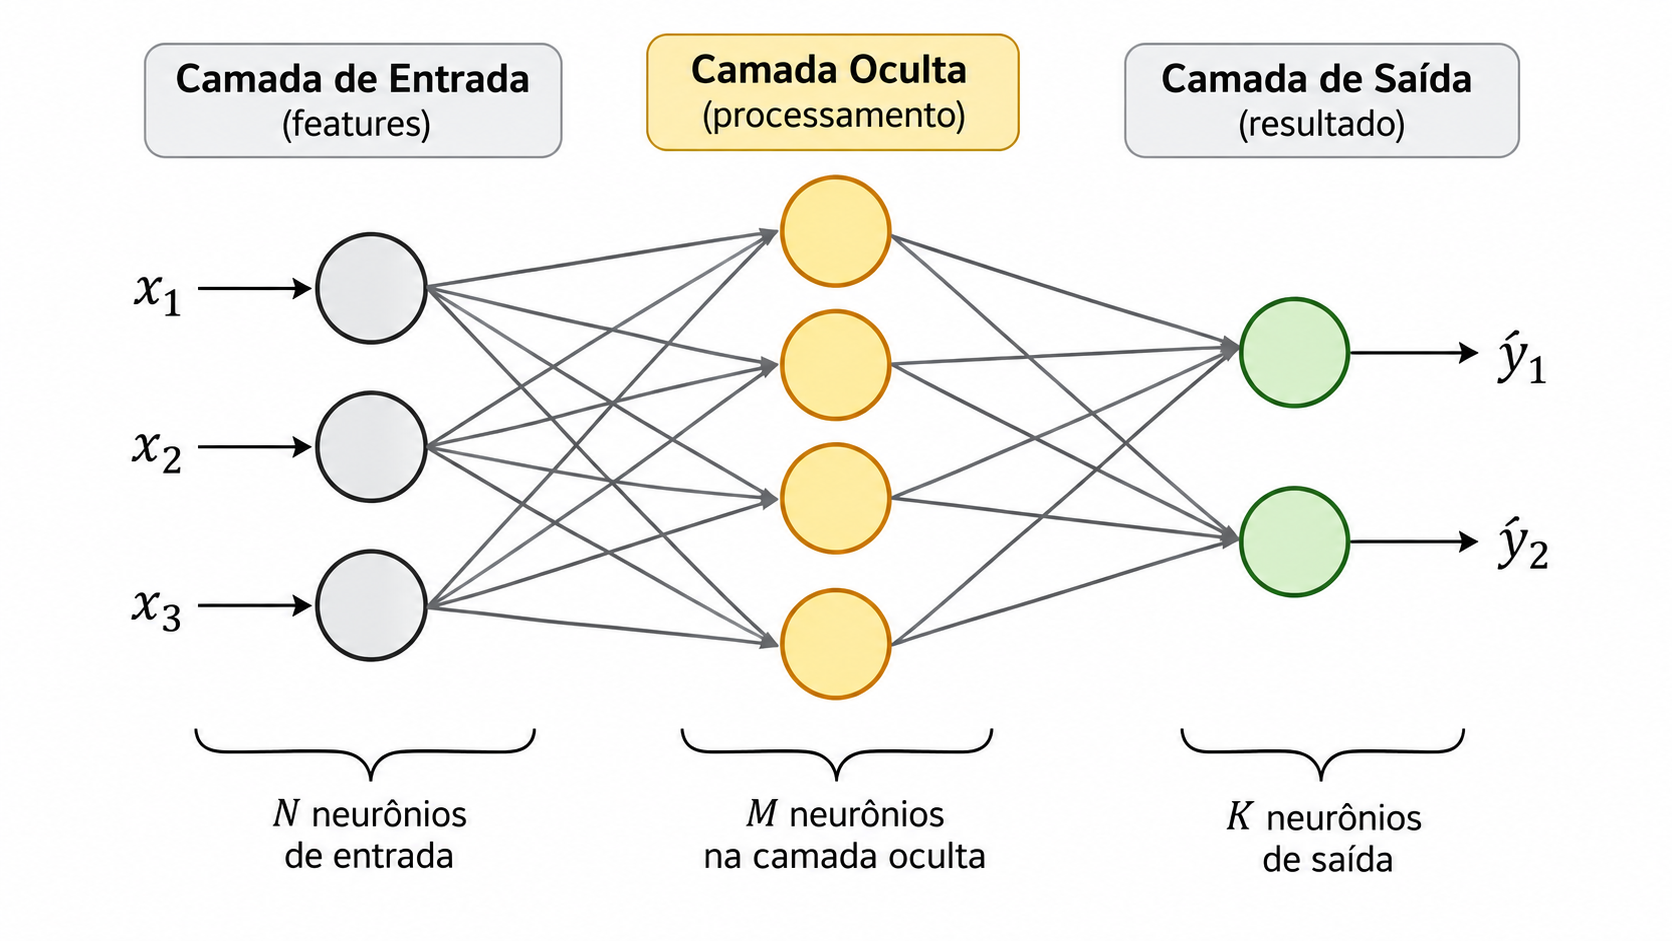
\includegraphics[width=0.85\textwidth]{sections/imagens/Grafo_Redes_Neurais.png}
    \small
    % Imagem com origem no Gemini
\end{figure}


\subsubsubsection{Redes Neurais Convolucionais}

Atualmente, as redes neurais convolucionais são amplamente aplicadas em processamento de dados não estruturados, 
como imagens, vídeos e áudios. Tal técnica tem como característica o 
processamento de pequenos trechos de dados por vez, ao contrário 
de outras técnicas que tentam realizar o processamento de forma atômica 
\cite{jesus2023inteligencia}.

Como apresentado por \citeonline{Atika2022ImageSegmentation}, 
o desenvolvimento de uma \gls{cnn} inicia-se pela definição da arquitetura em implementação. 
Tal técnica abrange uma vasta quantidade de arquiteturas que foram 
desenvolvidas para auxiliar e alcançar melhores resultados para 
determinados requisitos do software.

\subsubsubsection{Camadas que Constituem uma CNN} 
Uma \gls{cnn} é constituída por três principais camadas: camada de entrada de dados, 
camada de saída, também denominada camada densa, 
na qual cada um de seus neurônios está conectado à camada anterior, e diversas outras 
camadas intermediárias, 
denominadas por alguns autores camadas ocultas \cite{ayeni2022convolutional}. 

As camadas intermediárias de uma CNN 
apresentam comportamento de aprofundamento em reconhecimento de abstrações a cada camada sobreposta, 
de tal forma que as camadas iniciais são responsáveis por identificar traços, 
contornos, linhas etc., 
enquanto as camadas finais possuem a responsabilidade de identificar objetos, 
rostos e valores, por exemplo. 
Tais camadas são desenvolvidas com a intercalação de camadas de convolução e pooling (agrupamento), 
de forma que cada entrada de uma camada é a saída da camada anterior.

\paragraph{Camada Convolucional}
Como \citeonline{ayeni2022convolutional} explica, 
a camada convolucional é a camada responsável por processar imagens de forma 
a encontrar padrões ao aplicar um filtro (kernel/neurônio) a cada trecho 
da imagem de entrada, denominado campo receptivo. 
O neurônio é responsável por aplicar operações de multiplicação sobre o campo receptivo, 
gerando um único valor para cada trecho de imagem processado, 
e, posteriormente, os valores calculados pelos neurônios são 
armazenados em uma estrutura de três dimensões \cite{ayeni2022convolutional}.

A conversão da imagem para escala de cinza antes 
do processamento por uma \gls{cnn} é justificada 
por reduzir a complexidade cromática do padrão 
\gls{rgb} (três canais) para um canal único, 
o que impacta diretamente a profundidade dos kernels e o volume 
de parâmetros da primeira camada da rede 
\cite{ayeni2022convolutional}.

\paragraph{Camada de Pooling}
Segundo \citeonline{ayeni2022convolutional}, 
a camada de pooling possui a responsabilidade de filtrar características predominantes 
encontradas na camada de convolução. 
Tal camada possui a importantíssima função de otimizar processamento, 
descartando dados menos significativos 
e mitigando o fenômeno de overfitting.
As camadas de pooling possuem diversas derivações, que são 
escolhidas e implementadas a fim de otimizar resultados alcançados pelo modelo, 
mas a derivação mais aplicada sobre CNNs é a Max Pooling.

A operação de pooling reduz a resolução 
espacial dos mapas de características 
gerados pela camada convolucional, 
utilizando tipicamente uma janela de 
varredura (filtro) de $2 \times 2$.

\paragraph{Camada Totalmente Conectada}
Como \citeonline{ayeni2022convolutional} explica, 
a camada denominada Fully-Connected (Totalmente Conectada) possui a função de interpretar 
abstrações mais complexas da imagem e classificá-las. 
Essa camada possui todos os seus parâmetros conectados 
com os parâmetros da camada anterior, 
corriqueiramente resultando em um número de nós de saída 
igual à quantidade de classes de classificação.


\subsubsection{OCR - Fundamentos e Escopo}
O \gls{ocr} é um subcampo da Visão Computacional e da Inteligência Artificial 
dedicado à conversão de imagens contendo texto (impresso, manuscrito ou gravado) 
em dados legíveis por máquina \cite{chen2021survey}. 
Originalmente voltado à digitalização de documentos, 
o escopo foi ampliado pelo \textit{Deep Learning} 
para aplicações industriais e de IoT \cite{jawas2018water}.

\subsubsubsection{Pipeline Tradicional}
Um sistema clássico de OCR opera em etapas interdependentes \cite{chen2021survey}:
\begin{enumerate}
    \item \textbf{Aquisição e pré-processamento}: melhoria de contraste, correção de inclinação (\textit{deskewing}), remoção de ruído e binarização; em dispositivos embarcados, etapas de segmentação semântica podem isolar a Região de Interesse (ROI) antes do reconhecimento.
    \item \textbf{Localização e segmentação de texto}: identificação das regiões de texto.
    \item \textbf{Reconhecimento de caracteres}: classificação dos segmentos ou da sequência completa.
    \item \textbf{Pós-processamento}: dicionários, correção ortográfica ou verificação sintática para mitigar erros residuais.
\end{enumerate}

Em OCR, a leitura de uma palavra ou sequência numérica se beneficia do contexto em ambas as direções: o caractere atual é mais bem interpretado quando se conhece tanto o que veio antes quanto o que veio depois. 
Por isso, a CRNN emprega tipicamente camadas \textbf{bidirecionais} de LSTM (BiLSTM), que processam a sequência da esquerda para a direita e da direita para a esquerda e concatenam as representações resultantes \cite{shi2017crnn, hannun2017ctc}.

\subsubsubsection{Evolução Tecnológica: dos Métodos Heurísticos ao Deep Learning}
A literatura descreve três gerações principais \cite{chen2021survey}:

\subparagraph{Primeira geração (Template Matching).}
Sobreposição pixel a pixel com gabaritos estáticos; 
alta vulnerabilidade a variações de escala, rotação e fontes.

\subparagraph{Segunda geração (Características manuais + classificadores clássicos).}
Uso de descritores como HOG e SIFT, 
combinados com SVM ou MLP; dependência de \textit{feature engineering}.

\subparagraph{Terceira geração (End-to-End Deep Learning).}
Elimina a segmentação explícita de caracteres; 
modelos \textit{end-to-end} aprendem simultaneamente representações 
visuais e dependência contextual sequencial \cite{shi2017crnn}.


\subsubsection{Arquitetura U-Net - Segmentação de ROI}

Dado o objetivo da implementação de CNN neste trabalho, 
destaca-se a arquitetura U-Net. 

Como \citeonline{Atika2022ImageSegmentation} explicam,
a arquitetura U-Net tem por objetivo a definição de bordas dentro de imagens, 
sendo amplamente utilizada na biomedicina com o foco de delimitar 
estruturas presentes em imagens; tal característica é explorada a fim de definir 
\gls{roi} dentro de uma imagem.


\begin{figure}[H]
    \caption{Definição de ROI de uma Imagem}
    \label{fig: roi_definition_unet}
    \centering
    % Primeira Imagem
    \begin{subfigure}[b]{0.48\textwidth}
        \centering
        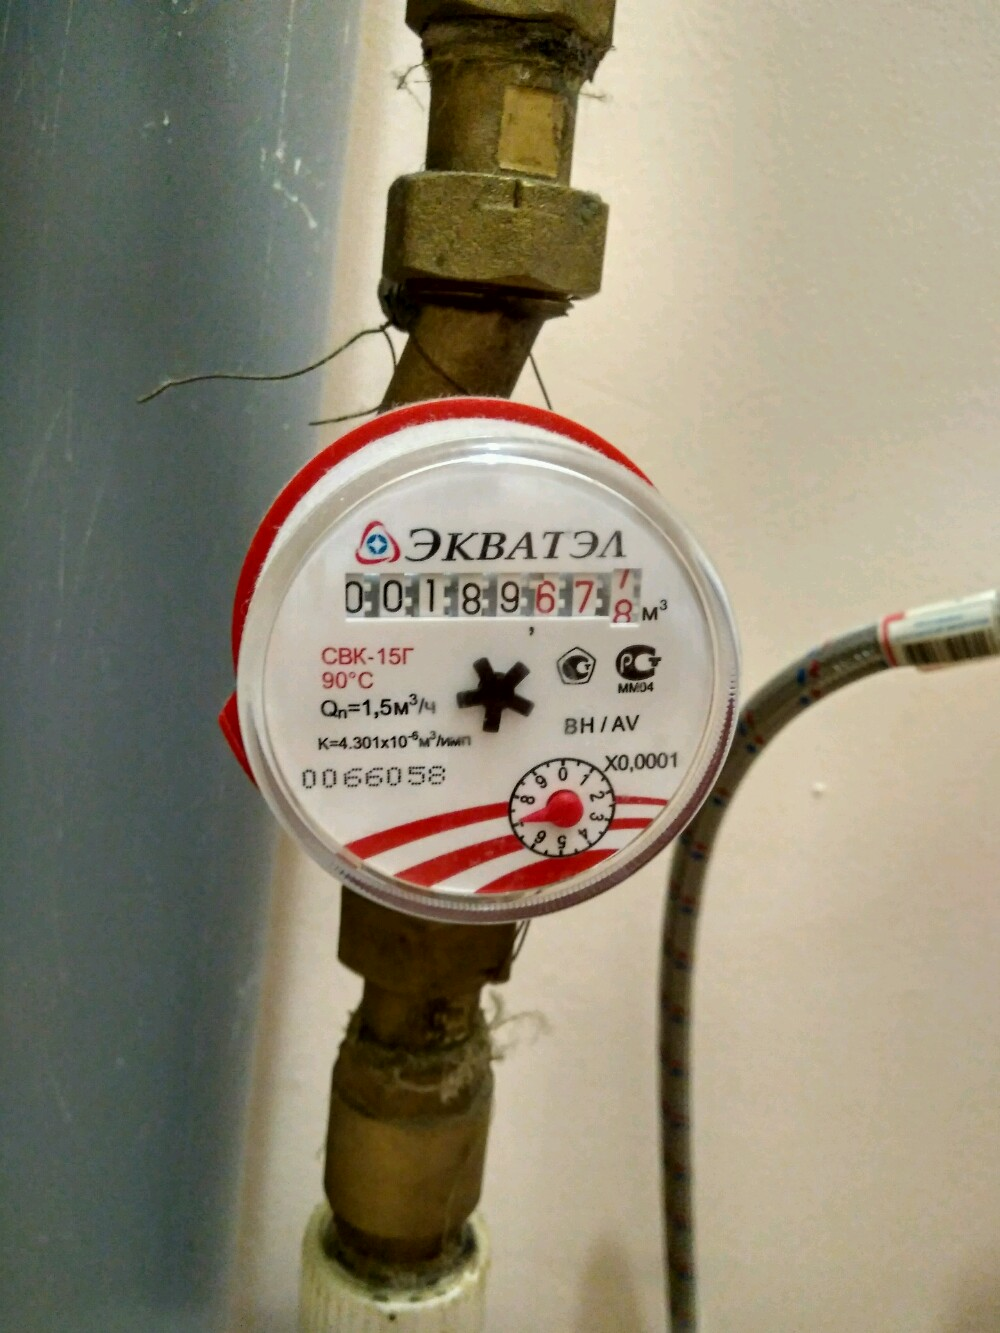
\includegraphics[width=\textwidth]{sections/imagens/Img_Original_Unet.jpg}
        \caption{Imagem Original}
        \label{fig:img1}
    \end{subfigure}\hfill % O \hfill fica colado no fechamento da primeira subfigura
    % Segunda Imagem
    \begin{subfigure}[b]{0.48\textwidth}
        \centering
        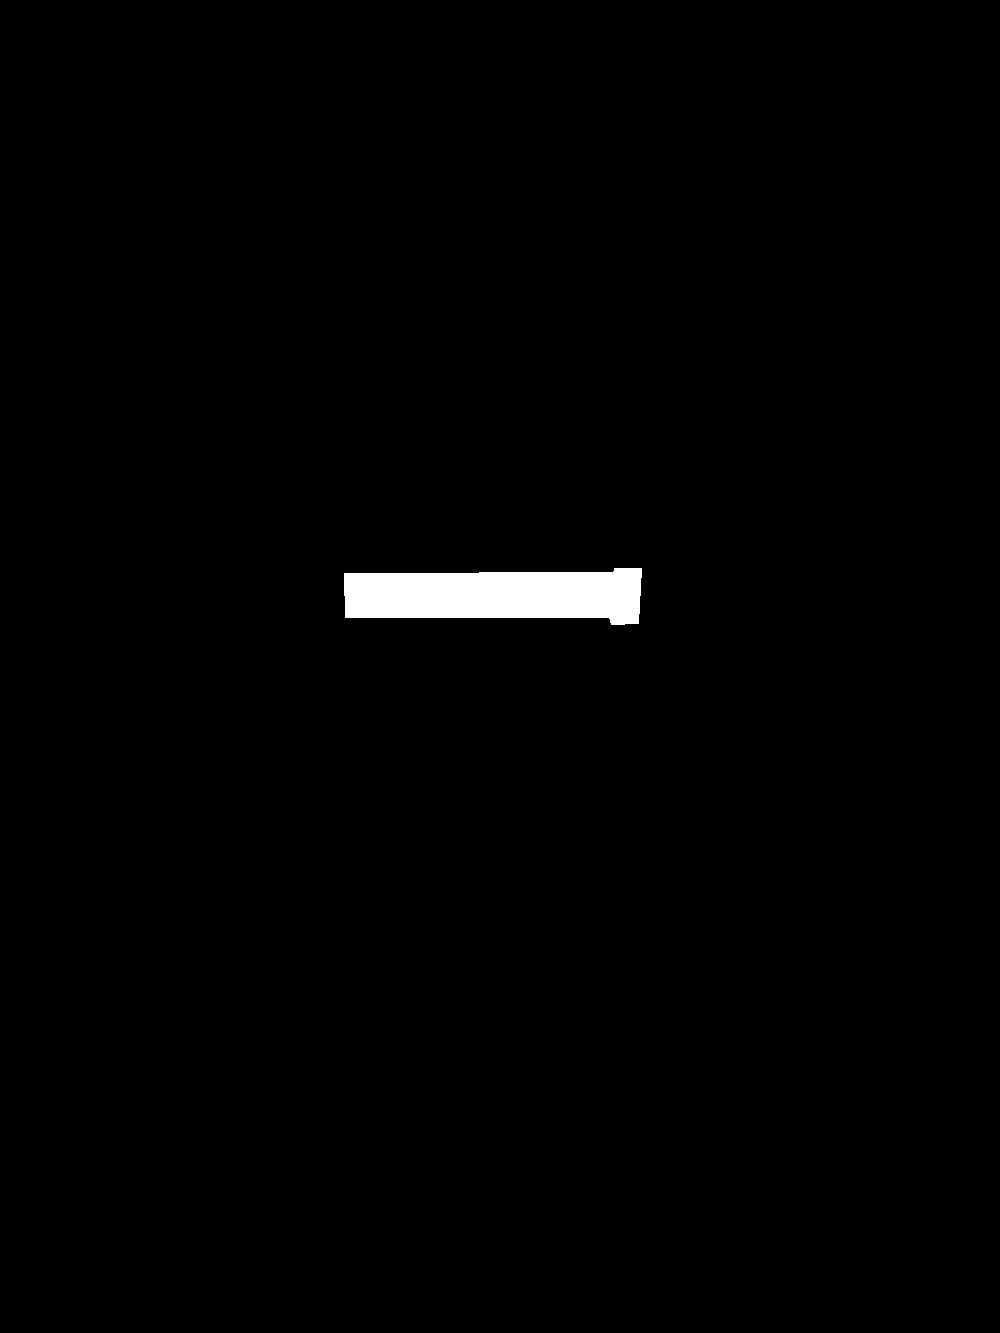
\includegraphics[width=\textwidth]{sections/imagens/Img_Mask_Unet.jpg}
        \caption{ROI Extraída da Imagem Original}
        \label{fig:img2}
    \end{subfigure}

    \fonte{Autores (2026).}
\end{figure}


A arquitetura U-Net é caracterizada pela presença de três etapas de 
processamento: Contração, Gargalo e Expansão. 
A camada de contração é composta por vários blocos, 
nos quais cada bloco recebe uma entrada e aplica uma camada de convolução seguida por 
uma camada de operação de max-pooling; essas camadas são matrizes 
que, respectivamente, apresentam a estrutura 3x3 e 2x2.

Com adendo, as camadas que constroem a arquitetura U-Net utilizam a função de ativação ReLU 
apresentada na equação~\ref{eq:relu_def}.

\begin{equation}
    f(x) = \text{ReLU}(x) = \max(0, x) = 
    \begin{cases} 
        x, & \text{se } x > 0 \\ 
        0, & \text{se } x \le 0 
    \end{cases}
    \label{eq:relu_def}
\end{equation}

\subsubsection{Arquitetura CRNN e CTC}
\label{subsubsec:crnn_ctc}
A arquitetura \gls{crnn} é amplamente utilizada em aplicações que exigem 
inferência de classes em sequência, 
pois combina um extrator convolucional (\gls{cnn}) 
a fim de obter representações visuais, 
uma camada recorrente (\gls{rnn}), com o objetivo de modelar dependências contextuais ao longo do eixo horizontal, 
e a função de perda \gls{ctc}, com a finalidade de alinhar as previsões da rede à sequência de rótulos sem a necessidade de 
segmentação explícita dos caracteres \cite{shi2017crnn}.

A técnica \gls{ctc} resolve o problema central de sequências de comprimento variável: 
em geral, não se sabe onde cada caractere começa e termina na imagem, 
e o número de \textit{frames} produzidos pela CNN é maior do que o número de caracteres 
da palavra ou número a ser reconhecido \cite{graves2006ctc}. 
Para lidar com isso, a técnica CTC introduz dois mecanismos fundamentais: 
um \textit{token} oculto de espaçamento (\textit{blank}) e uma 
função de colapso que mapeia a sequência de previsões da rede 
para o rótulo final \cite{graves2006ctc, hannun2017ctc}.

\subparagraph{O \textit{token} \textit{blank} e o colapso de repetições.}
A cada passo de tempo, 
a rede produz uma distribuição de probabilidade sobre o alfabeto 
acrescido do símbolo especial \textit{blank} (\(\epsilon\)). 
O \textit{blank} representa a ausência de emissão de caractere naquele instante, 
funcionando como um separador entre caracteres idênticos adjacentes 
\cite{graves2006ctc}. 
Após a rede produzir a sequência completa de previsões, 
aplica-se uma função de colapso \(\mathcal{B}\) 
que (i) remove caracteres repetidos consecutivos e 
(ii) remove os \textit{blanks} \cite{hannun2017ctc}. 
Por exemplo, a sequência de caminho \(--h--e--l--l--o--\) colapsa 
para \(\text{``hello''}\); 
sem o \textit{blank}, as repetições de ``l'' seriam indistinguíveis de 
um único ``l'' \cite{hannun2017ctc}.

\subparagraph{Marginalização de alinhamentos.}
O treinamento da CTC não exige um alinhamento predefinido entre 
os \textit{frames} e os caracteres. Em vez disso, 
a função de perda calcula a probabilidade da sequência de rótulos correta como 
a soma das probabilidades de todos os caminhos de alinhamento válidos que, após o colapso, 
produzem aquele rótulo \cite{graves2006ctc}. 
Essa marginalização é feita de forma eficiente pelo algoritmo \textit{forward-backward}, 
que explora a estrutura do problema para evitar a 
enumeração explícita de todos os caminhos, 
que seria computacionalmente inviável \cite{graves2006ctc, hannun2017ctc}. 
Assim, a rede pode ser treinada diretamente com pares (imagem, transcrição), 
sem anotações de posição caractere a caractere.

\subparagraph{Inferência.}
No momento da inferência, a rede produz, para cada passo de tempo, 
a classe mais provável (ou uma distribuição sobre as classes). 
A sequência final é obtida pelo colapso das previsões, 
opcionalmente combinado com busca em feixe (\textit{beam search}) 
para explorar múltiplos alinhamentos e melhorar a acurácia \cite{hannun2017ctc}. 
O artigo de Hannun (2017) apresenta uma explicação visual detalhada desse processo, 
incluindo exemplos passo a passo de como o \textit{blank} e o 
colapso atuam em sequências reais \cite{hannun2017ctc}.

\subparagraph{Por que a CTC é adequada ao OCR.}
Em OCR de palavras, números de medidores ou placas, 
o número de caracteres varia e não há garantia de que 
cada caractere ocupe exatamente um número fixo de \textit{frames} 
na saída da CNN. 
A CTC elimina a necessidade de segmentação manual e permite que a 
CRNN seja treinada de ponta a ponta com sequências de comprimentos diferentes, 
mantendo a coerência entre as previsões vizinhas e evitando 
o colapso de repetições idênticas \cite{shi2017crnn, graves2006ctc}.

\subsubsection{Quantização e QAT}
Quantização é um método de simplificação dos parâmetros de um modelo de \gls{rna}. 
Como \citeonline{ferreira2022compressao} explica, a aplicação de tal técnica 
traz como benefício a redução do tamanho de modelos, 
viabilizando a utilização em equipamentos de baixo poder computacional, 
além do aumento de velocidade de inferência e simplificação de cálculos realizados pelo processador, 
frente a um modelo que, na maioria dos casos, possui seus parâmetros representados em pontos 
flutuantes de 32 bits. 

A técnica \gls{qat}, com foco em transformação de parâmetros para inteiros de 8 bits,
simula a perda de precisão da conversão de FP32 para INT8 durante o treinamento, 
permitindo que os pesos da rede se adaptem e mitiguem a degradação de acurácia.
Em sistemas de OCR para medidores, 
modelos quantizados alcançam tamanhos da ordem de centenas de kB e 
inferência em subsegundo em hardware embarcado 
\cite{ademola2023resource, jawas2018water}.





% ---------------------------------------------------------------
\section{Trabalhos correlatos}
\label{sec:trabalhos_correlatos}
Nesta seção, analisam-se pesquisas que utilizam IoT e Visão Computacional para a digitalização de medidores de consumo, como as soluções de computação de borda propostas por \citeonline{SilvaVilela2021} e \citeonline{bravo2025ants}, além de arquiteturas de sensores inteligentes exploradas por \citeonline{Tedjojuwono2024}. 
O objetivo é contextualizar as escolhas arquiteturais deste TCC, comparando modelos de processamento (borda vs nuvem) e protocolos de comunicação sem fio. 
A revisão fundamenta o estado da técnica e destaca os diferenciais desta proposta em termos de infraestrutura de dados e eficiência energética.

\subsection{Trabalho 1: Solução IoT para Digitalização de Medidores de Consumo por Visão Computacional e MicroML}

\citeonline{SilvaVilela2021} abordou o tema de soluções IoT para Medidores de Consumo. 
Para resolvê-lo, foi desenvolvido um sistema utilizando microprocessadores ESP32, baseado no método de \gls{edge_computing}. O autor desenvolveu um software próprio, otimizado para microprocessadores, focado em \gls{ocr}, extraindo os dados, transmitindo-os via rede \gls{lorawan} e armazenando-os localmente; posteriormente, os dados são apresentados em um simples dashboard apresentando o consumo extraído pelo sistema até o momento. 

A metodologia utilizada foi a pesquisa experimental, na qual houve o desenvolvimento de um sistema que supre a necessidade de extração de dados de maneira digital. 

Os resultados mostraram que o desenvolvimento deste tipo de ferramenta é totalmente viável e, em suma, o experimento foi bem-sucedido. 
No entanto, a solução apresenta limitações, principalmente no que tange ao desenvolvimento do dataset, no qual não foi implementado tratamento adequado ao enviesamento dos dados. 
Também existe uma carência de métricas para medição de consumo energético e de processamento pelo sistema.

O presente trabalho diferencia-se por aplicar uma comparação entre uma arquitetura clássica de Edge vs Cloud, e um ponto que atacamos mais profundamente é a apresentação de métricas importantíssimas no desenvolvimento de um sistema IoT além da acurácia de modelo, por exemplo, as métricas de consumo energético e impactos em manutenção por decisões tomadas. 

\subsection{Trabalho 2: Sistema de Gerenciamento Inteligente de Água Utilizando Sensores Baseados em IoT}

\citeonline{Tedjojuwono2024} abordaram o tema de sistemas inteligentes para o manejo de recursos hídricos em áreas residenciais. 
Para resolvê-lo, os autores propuseram o desenvolvimento de um framework que substitui medidores mecânicos por sensores de fluxo eletrônicos integrados a uma arquitetura IoT. 
O sistema utiliza prototipagem com Arduino Uno e sensores de efeito Hall (YF-S201) para coletar dados de vazão em tempo real, enviando as informações via módulo 3G/GPRS para um servidor de banco de dados centralizado. 
Os dados processados alimentam uma aplicação web que permite o monitoramento do consumo, faturamento automatizado e a detecção precoce de anomalias na distribuição.

A metodologia utilizada seguiu os princípios do Design Thinking, incluindo uma fase qualitativa de coleta de requisitos através de entrevistas com usuários e a criação de mapas de empatia, seguida pelo desenvolvimento do protótipo e avaliação de usabilidade através da escala SUS (System Usability Scale). 

Os resultados mostraram que a solução é viável e intuitiva, obtendo uma pontuação média de 72 na escala SUS, o que indica uma boa aceitação pelos usuários. 
No entanto, o trabalho aponta limitações na abrangência dos dados, focando primariamente na taxa de fluxo, e destaca a necessidade de integrar mais tipos de sensores (como pressão e qualidade da água) para análises de Big Data mais robustas. 
Além disso, a precisão total do sistema de previsão depende de um volume maior de dados históricos que ainda precisam ser coletados. 

O presente trabalho diferencia-se por focar na infraestrutura de comunicação \gls{lorawan}, visando uma maior eficiência energética e alcance em comparação ao GPRS/3G utilizado pelos autores, além de explorar a integração direta com medidores analógicos já existentes através de telemetria, em vez da substituição completa do hardware de medição. 

\subsection{Trabalho 3: Rede de Sensores Sem Fio Habilitada para LoRa para Leitura e Faturamento de Consumo de Água Usando Reconhecimento Óptico de Caracteres}

\citeonline{bravo2025ants} desenvolveram um sistema automatizado para leitura de hidrômetros 
analógicos utilizando uma combinação de tecnologias de baixo custo e comunicação de longo alcance.
O objetivo central foi mitigar erros humanos e atrasos operacionais comuns em leituras manuais.

A metodologia consistiu na integração de um módulo \gls{esp32cam} para captura de 
imagens dos medidores e um algoritmo de \gls{ocr} 
para a extração digital dos dados de consumo no próprio dispositivo. 
Para a transmissão, utilizou-se a tecnologia \gls{lora} (módulo Ra-02), 
operando em uma topologia de rede que inclui repetidores para estender 
o alcance e um gateway central para envio dos dados à nuvem. 
O sistema também implementou estratégias de gerenciamento de energia através 
de ciclos de \textit{deep sleep} programados para aumentar a vida útil da bateria.

Os resultados apontaram uma precisão de 99,71\% no reconhecimento 
dos dígitos e um alcance de transmissão estável de até 1070 metros em condições de campo aberto. 
Os autores observaram que medidores mais antigos ou obstruídos podem elevar o tempo de processamento do \gls{ocr}.

O presente trabalho diferencia-se diante dos seguintes tópicos:

\begin{itemize}
	\item Metodologia de Pesquisa: \citeonline{bravo2025ants}, aplicaram em seu trabalho a metodologia \gls{dsr}, 
    desenvolvendo uma solução à problemática da coleta de dados em hidrômetros, 
    em contrapartida, este trabalho possui como objetivo a comparação entre métodos 
    de processamento de dados em sistemas IOT.
	
    \item Público-Alvo: O trabalho correlato, busca impactar principalmente empresas consorciadas à 
    distribuição de recursos hídricos. O presente trabalho busca impactar desenvolvedores de sistemas IOT, 
    ao prover dados comparativos que podem pautar decisões arquitetônicas de novos sistemas.
	
    \item Especificação de Restrições Regulatórias: Este trabalho utiliza como base a regulação AU915, 
    adotada pela ANATEL em 2017. O trabalho de \citeonline{bravo2025ants}, 
    não define qual restrição regulatória o sistema está seguindo, 
    o que impacta diretamente sobre a viabilidade de operação do sistema desenvolvido.
\end{itemize}

Utilizaremos esse trabalho como referência no desenvolvimento do fluxo de borda 
para realizar uma comparação com a abordagem de processamento em nuvem, 
contribuindo para a discussão sobre o trade-off entre eficiência 
energética e precisão em sistemas de telemetria de baixo custo.


% ===============================================================
% CAPÍTULO 3 - DESENVOLVIMENTO
% ===============================================================
\chapter{Desenvolvimento}
\label{cap:desenvolvimento}

% ---------------------------------------------------------------
\section{Metodologia da pesquisa}
\label{sec:metodologia_pesquisa}
Para avaliar a eficácia do sistema de telemetria proposto e garantir a objetividade dos resultados, 
foram adotados indicadores quantitativos divididos em três dimensões críticas: desempenho de rede, 
precisão de visão computacional, eficiência energética e acurácia preditiva.

\subsection{Desempenho da Rede de Comunicação}
A robustez da transmissão via \gls{lorawan} será quantificada através da \gls{pdr}. 
Conforme a metodologia de \citeonline{bravo2025ants}, 
o PDR é definido pela razão entre o número de pacotes recebidos 
pelo \textit{gateway} e o número de pacotes enviados pelo nó sensor:

\begin{equation}
\label{eq:pdr}
PDR = \left( \frac{\text{Pacotes Recebidos}}{\text{Pacotes Enviados}} \right) \times 100
\end{equation}

Além do \gls{pdr}, será medida a latência de ponta a ponta, 
compreendendo o tempo decorrido desde o disparo da captura da imagem no ESP32 
até a disponibilidade do dado processado no \textit{dashboard}.

% =================================================================================================

\subsection{Acurácia da Visão Computacional (OCR)}

A validação do algoritmo de \gls{ocr}, 
responsável pela extração dos dígitos dos medidores, 
será realizada sob diferentes condições de iluminação e 
ângulos de captura, 
visando simular cenários reais de instalação. 

Conforme discutido por \citeonline{barkat2024smart}, 
a eficácia de modelos de \textit{Deep Learning} 
aplicados ao monitoramento deve ser medida 
pela sua capacidade de generalização. 
Para este trabalho, a métrica principal será a Acurácia de Leitura ($Acc_{ocr}$),
definida pela razão entre as predições que coincidem exatamente com o valor real (verdade de campo) 
e o total de amostras testadas:

\begin{equation}
Acc_{ocr} = \frac{VP + VN}{VP + VN + FP + FN}
\end{equation}

Em que $VP$, $VN$, $FP$ e $FN$ representam, respectivamente,
os Verdadeiros Positivos, Verdadeiros Negativos, Falsos Positivos 
e Falsos Negativos obtidos através da Matriz de Confusão. 
Esta abordagem quantitativa permite identificar se erros de 
leitura estão associados a fatores externos, como reflexos na cúpula 
de vidro do medidor ou distorções de perspectiva.

% =================================================================================================

\subsection{Autonomia Energética}
A eficiência do hardware será validada através da 
medição do consumo de corrente em diferentes estados de 
operação (\textit{Deep Sleep}, captura de imagem e transmissão). 
A autonomia estimada ($A$) em dias será calculada pela relação 
entre a capacidade da bateria ($C_{bat}$) 
e o consumo médio diário ($I_{médio}$):

\begin{equation}
A = \frac{C_{bat}}{I_{médio} \times 24}
\end{equation}


\section{Detalhes da implementação}
\label{sec:implementacao}
\subsection{Visão geral da solução}
\label{subsec:visao_geral}

O sistema desenvolvido realiza a leitura automática de hidrômetros analógicos do tipo
ciclométrico, cujo mostrador é formado por roletes numerados, por meio de um nó sensor
baseado no \gls{esp32cam}. O nó fotografa o mostrador do medidor e envia o resultado,
via \gls{lorawan}, até uma estação receptora conectada a um computador, que faz o papel
de servidor da aplicação.

Para responder à pergunta de pesquisa, o mesmo nó foi implementado em dois fluxos de
processamento, que diferem no local em que o \gls{ocr} é executado e, por consequência,
no conteúdo que trafega pelo enlace:

\begin{itemize}
    \item \textbf{Fluxo em nuvem} (\gls{cloud_computing}): o nó captura a imagem, comprime-a
    no formato JPEG e a transmite fragmentada em blocos. O servidor remonta a imagem e
    executa o reconhecimento dos dígitos.
    \item \textbf{Fluxo em borda} (\gls{edge_computing}): o nó captura a imagem, executa
    localmente os modelos de reconhecimento e transmite apenas a leitura resultante, em um
    único pacote de 9 bytes.
\end{itemize}

Uma decisão central da implementação é que os dois fluxos utilizam os mesmos modelos de
redes neurais, quantizados em inteiros de 8 bits (INT8), e a mesma lógica de leitura.
Assim, as diferenças de latência, entrega de pacotes e consumo energético observadas entre
eles decorrem apenas do local de processamento e do volume de dados transmitido, e não de
modelos com capacidades distintas. O efeito da quantização sobre a acurácia, objeto da
hipótese H1, é avaliado à parte, pela comparação entre as versões em ponto flutuante de
32 bits e em INT8 do mesmo modelo.

A Figura~\ref{fig:arquitetura_geral} apresenta a arquitetura do sistema e o caminho
percorrido pelos dados em cada fluxo.

\begin{figure}[H]
    \centering
    \caption{Arquitetura do sistema e os dois fluxos de processamento}
    \label{fig:arquitetura_geral}
    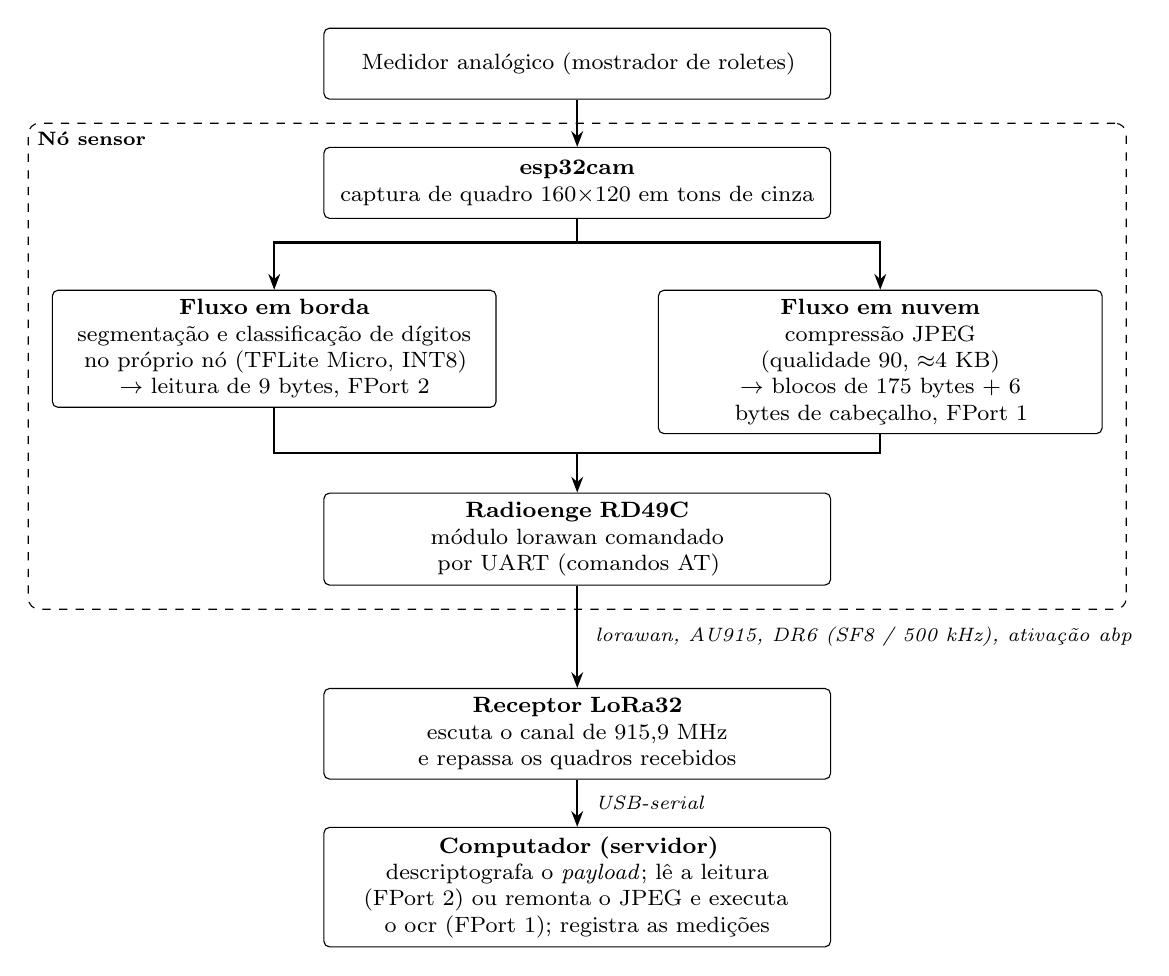
\begin{tikzpicture}[
        font=\footnotesize,
        node distance=6mm and 6mm,
        bloco/.style={draw, rounded corners=2pt, align=center, fill=white,
                      minimum height=9mm, text width=#1},
        bloco/.default=6.2cm,
        seta/.style={-{Stealth[length=2mm]}, thick},
        rotulo/.style={font=\scriptsize\itshape, align=center}
    ]
        \node[bloco] (hidro) {Medidor analógico (mostrador de roletes)};
        \node[bloco, below=of hidro] (cam)
            {\textbf{\gls{esp32cam}}\\captura de quadro 160$\times$120 em tons de cinza};
        \node[bloco=5.4cm, below left=9mm and -2.2cm of cam] (borda)
            {\textbf{Fluxo em borda}\\segmentação e classificação de dígitos no
             próprio nó (TFLite Micro, INT8)\\$\rightarrow$ leitura de 9 bytes, FPort 2};
        \node[bloco=5.4cm, below right=9mm and -2.2cm of cam] (nuvem)
            {\textbf{Fluxo em nuvem}\\compressão JPEG (qualidade 90, $\approx$4~KB)\\
             $\rightarrow$ blocos de 175 bytes + 6 bytes de cabeçalho, FPort 1};
        \node[bloco] (radio) at ($(borda.south)!0.5!(nuvem.south)+(0,-15mm)$)
            {\textbf{Radioenge RD49C}\\módulo \gls{lorawan} comandado por UART (comandos AT)};
        \node[draw, dashed, rounded corners=4pt, inner sep=3mm,
              fit=(cam) (borda) (nuvem) (radio),
              label={[font=\scriptsize\bfseries, anchor=north west]north west:Nó sensor}] (no) {};
        \node[bloco, below=13mm of radio] (rx)
            {\textbf{Receptor LoRa32}\\escuta o canal de 915,9~MHz e repassa os quadros recebidos};
        \node[bloco, below=of rx] (pc)
            {\textbf{Computador (servidor)}\\descriptografa o \textit{payload}; lê a leitura
             (FPort 2) ou remonta o JPEG e executa o \gls{ocr} (FPort 1); registra as medições};

        \draw[seta] (hidro) -- (cam);
        \draw[seta] (cam.south) -- ++(0,-3mm) -| (borda.north);
        \draw[seta] (cam.south) -- ++(0,-3mm) -| (nuvem.north);
        \draw[thick] (borda.south) |- ([yshift=5mm]radio.north);
        \draw[thick] (nuvem.south) |- ([yshift=5mm]radio.north);
        \draw[seta] ([yshift=5mm]radio.north) -- (radio.north);
        \draw[seta] (radio) -- node[rotulo, right=1mm]
            {\gls{lorawan}, AU915, DR6 (SF8 / 500~kHz), ativação \gls{abp}} (rx);
        \draw[seta] (rx) -- node[rotulo, right=1mm] {USB-serial} (pc);
    \end{tikzpicture}
    \legend{Fonte: Elaborado pelos autores (2026).}
\end{figure}

\subsection{Componentes de hardware}
\label{subsec:hardware}

O protótipo foi montado com componentes de baixo custo. A Tabela~\ref{tab:hardware} resume a função de cada um.

\begin{table}[H]
    \centering
    \caption{Componentes de hardware do protótipo}
    \label{tab:hardware}
    \begin{tabularx}{\textwidth}{@{}lX@{}}
        \toprule
        \textbf{Componente} & \textbf{Função no sistema} \\
        \midrule
        \gls{esp32cam} (AI-Thinker) & Nó sensor. Microcontrolador ESP32 a 240~MHz com 4~MB de PSRAM e
        câmera integrada. Captura a imagem e, no fluxo em borda, executa os modelos de \gls{ocr}. \\
        Radioenge RD49C & Módulo \gls{lorawan} homologado pela ANATEL, ligado ao \gls{esp32cam} por UART
        (GPIO~15 e GPIO~14) e controlado por comandos AT. Opera no plano AU915 com potência de até
        +20~dBm. \\
        Heltec/TTGO LoRa32 V2 & Receptor. Rádio LoRa configurado no mesmo canal e na mesma taxa do
        transmissor; repassa cada quadro recebido ao computador pela porta serial, junto com o
        RSSI. \\
        Computador & Servidor da aplicação. Descriptografa os quadros, remonta as imagens,
        executa o \gls{ocr} do fluxo em nuvem e registra as medições. Também foi usado no
        treinamento dos modelos. \\
        INA219 e Arduino Uno & Instrumentação. Sensor de corrente com resistor \textit{shunt} de
        0,1~$\Omega$, lido por um Arduino Uno a 100 amostras por segundo, usado para medir o
        consumo do nó sensor. \\
        \bottomrule
    \end{tabularx}
    \legend{Fonte: Elaborado pelos autores (2026).}
\end{table}

\subsection{Componentes de software}
\label{subsec:software}

O código do projeto está reunido em um único repositório\footnote{Disponível em
\url{https://github.com/Marcelo-122/Codigo-do-TCC2}.} e se divide em firmwares para os
microcontroladores, escritos em C++ com o \textit{core} Arduino-ESP32 3.0.7, e
\textit{scripts} em Python executados no computador. A Tabela~\ref{tab:software} relaciona
os principais componentes.

\begin{table}[H]
    \centering
    \caption{Principais componentes de software}
    \label{tab:software}
    \begin{tabularx}{\textwidth}{@{}lX@{}}
        \toprule
        \textbf{Componente} & \textbf{Responsabilidade} \\
        \midrule
        \texttt{transmissor\_esp32cam} & Firmware do nó no fluxo em nuvem: captura, compressão JPEG,
        fragmentação e envio dos blocos pela porta 1 (FPort 1). \\
        \texttt{transmissor\_ocr\_esp32cam} & Firmware do nó no fluxo em borda: captura, inferência dos
        modelos com TensorFlow Lite Micro e envio da leitura pela porta 2 (FPort 2). \\
        \texttt{receptor\_lora32} & Firmware do receptor: escuta o canal e escreve na serial cada
        quadro recebido. \\
        \texttt{reconstrutor.py}, \texttt{enlace.py} & Lado do servidor: leitura da serial,
        descriptografia, remontagem da imagem ou decodificação da leitura e registro das medições. \\
        \texttt{ocr/pipeline\_nuvem.py} & \gls{ocr} do fluxo em nuvem, com os mesmos modelos e a
        mesma lógica do firmware de borda. \\
        \texttt{ModeloEDataset/} & Preparação dos conjuntos de dados, treinamento, quantização e
        exportação dos modelos para o firmware. \\
        \texttt{medicoes/} & \textit{Scripts} de medição de corrente e de latência e os dados
        brutos coletados. \\
        \bottomrule
    \end{tabularx}
    \legend{Fonte: Elaborado pelos autores (2026).}
\end{table}

Nos dois fluxos, os firmwares do nó compartilham o mesmo rádio, a mesma configuração de
enlace, o mesmo ciclo de \textit{deep sleep} e o mesmo formato de registro de tempos, de
modo que as medições de consumo e de latência sejam obtidas pelos mesmos \textit{scripts}
e possam ser comparadas diretamente.

\subsection{Simplificações em relação a uma implantação real}
\label{subsec:simplificacoes}

Algumas escolhas do protótipo simplificam a infraestrutura descrita na
Seção~\ref{sec:fundamentos} e devem ser consideradas na interpretação dos resultados:

\begin{itemize}
    \item \textbf{Receptor de canal único no lugar de um \textit{gateway}}: o receptor LoRa32
    escuta um único canal, fixo, e não implementa as funções de um \textit{gateway}
    \gls{lorawan} multicanal. Por isso, o transmissor também foi configurado para usar um
    único canal (Seção~\ref{subsec:enlace}).
    \item \textbf{Ausência de servidor de rede}: não há servidor de rede nem servidor de
    aplicação dedicados. O dispositivo usa ativação \gls{abp}, com chaves de sessão
    configuradas previamente, e o próprio computador descriptografa o \textit{payload} com a
    chave de aplicação (AppSKey). O código de integridade da mensagem (MIC) não é verificado,
    pois exigiria a chave de rede. Um protótipo inicial, que injetava os pacotes em um
    servidor ChirpStack sem uso de rádio, foi descartado.
    \item \textbf{Ambiente de bancada}: as medições de enlace foram feitas com transmissor e
    receptor a poucos metros de distância, com sinal forte, de modo que avaliam o
    comportamento dos fluxos, e não o alcance do enlace.
\end{itemize}

\subsection{Enlace LoRaWAN}
\label{subsec:enlace}

Esta seção descreve a configuração do enlace de rádio, o formato das mensagens trocadas
nos dois fluxos, o preparo e a fragmentação da imagem e o tratamento dos quadros
recebidos pelo servidor. Os mesmos parâmetros de rádio foram usados nos dois fluxos.

\subsubsection{Estudo preliminar e escolha da configuração de rádio}
\label{subsubsec:estudo_preliminar_enlace}

Na fase inicial do trabalho, a viabilidade do envio de imagens foi estimada
analiticamente para o plano AU915 com canais de 125~kHz e \gls{sf}~8. Nessa configuração,
o Ato n\textordmasculine~14.448 da ANATEL enquadra o \gls{lora} como sistema de salto em
frequência, que deve usar no mínimo 35 canais e limitar o tempo médio de ocupação de cada
canal a 0,4~s em um intervalo de 14~s \cite{anatel2017}. Para respeitar esse limite, cada
pacote foi restrito a 115~bytes na camada física; com isso, uma imagem JPEG de 3.182~bytes
exigiria 38 pacotes de 348,7~ms cada, totalizando cerca de 13,3~s de rádio ativo.

Essa configuração foi abandonada na implementação por dois motivos. Primeiro, o salto
entre pelo menos 35 canais é incompatível com o receptor disponível, que escuta um único
canal (Seção~\ref{subsec:simplificacoes}). Segundo, o limite de 400~ms por transmissão
restringe o tamanho do bloco de dados: um pacote com 181~bytes de \textit{payload},
tamanho adotado adiante, ocuparia 543~ms de rádio com 125~kHz.

Por isso, o enlace foi configurado para operar com largura de banda de 500~kHz, no
\textit{data rate} DR6 do plano AU915, que corresponde a SF8 com 500~kHz
(Tabela~\ref{tab:uplink_datarate}) e a um \textit{payload} máximo de 222~bytes
\cite{radioenge2022}. Com essa largura de banda, o rádio se enquadra no item~10.3 do mesmo
Ato, destinado a sistemas de modulação digital (Seção~\ref{subsec:restricoes_regulatorias}),
cujos três requisitos são verificados a seguir: largura de faixa a 6~dB de, no mínimo,
500~kHz; potência de pico máxima de 1~W; e densidade espectral de potência máxima de 8~dBm
em qualquer faixa de 3~kHz.

O módulo Radioenge RD49C transmite com potência máxima de +20~dBm (100~mW), sem comando AT
que permita ajustá-la \cite{radioenge2022}, abaixo do limite de 1~W. Supondo que essa potência se distribua de forma plana pelos 500~kHz, a densidade
espectral fica em torno de
$20 - 10\log_{10}(500/3) \approx -2{,}2$~dBm em 3~kHz, abaixo do limite de 8~dBm. Por ser
enquadrado no item~10.3, o sistema dispensa o salto de frequência e o limite de ocupação
por canal exigidos para os canais de 125~kHz, o que permite usar um canal fixo. O módulo é
homologado pela ANATEL (certificado n\textordmasculine~02021-18-07215), mas duas ressalvas
se aplicam: a largura de faixa a 6~dB do sinal \gls{lora} com 500~kHz nominais não consta
do manual e deve ser confirmada nos ensaios de homologação, e antenas com ganho superior a
6~dBi exigiriam a redução da potência (item 10.5).

O canal escolhido foi o de 915,9~MHz, o primeiro canal de 500~kHz do plano AU915: canal
64 na numeração da especificação \cite{lora_alliance_rp002_105}, que começa em zero, e
canal 65 na numeração do manual do módulo, que começa em um. No módulo, ele foi
selecionado pela máscara de canais (\texttt{AT+CHMASK}), e o \textit{data rate} foi fixado
em DR6 com o ajuste adaptativo de taxa (ADR) desativado, pois o comando \texttt{AT+DR} só
tem efeito com o ADR desligado \cite{radioenge2022}. A Tabela~\ref{tab:parametros_enlace} reúne os parâmetros
usados por todos os componentes do enlace.

\begin{table}[H]
    \centering
    \caption{Parâmetros do enlace LoRaWAN}
    \label{tab:parametros_enlace}
    \begin{tabularx}{\textwidth}{@{}lX@{}}
        \toprule
        \textbf{Parâmetro} & \textbf{Valor} \\
        \midrule
        Plano de canais & AU915 \\
        Canal & Fixo, 915,9~MHz (canal 64), sem salto de frequência \\
        \textit{Data rate} & DR6: \gls{sf}~8, \gls{bw} de 500~kHz, ADR desativado \\
        Camada física & \gls{cr} 4/5, preâmbulo de 8 símbolos, CRC ativado, cabeçalho
        explícito, palavra de sincronismo \texttt{0x34} \\
        Potência de transmissão & +20~dBm (fixa no módulo) \\
        Ativação & \gls{abp} \\
        \textit{Payload} máximo em DR6 & 222~bytes \\
        Portas de aplicação & FPort~1 (blocos de imagem) e FPort~2 (leitura do \gls{ocr}) \\
        Bloco de imagem & 175~bytes de dados + 6~bytes de cabeçalho = 181~bytes \\
        Intervalo entre pacotes & 7~s \\
        \bottomrule
    \end{tabularx}
    \legend{Fonte: Elaborado pelos autores (2026).}
\end{table}

\subsubsection{Formato das mensagens}
\label{subsubsec:formato_mensagens}

Cada mensagem \gls{lorawan} acrescenta 13~bytes ao conteúdo da aplicação: o cabeçalho MAC
(1~byte), o endereço do dispositivo (4~bytes), o campo de controle (1~byte), o contador de
quadros FCnt (2~bytes), a porta de aplicação FPort (1~byte) e o código de integridade MIC
(4~bytes). O conteúdo da aplicação (FRMPayload) é criptografado com a chave de sessão de
aplicação (AppSKey). Os dois fluxos usam portas diferentes, o que permite ao servidor
distinguir as mensagens sem nenhum outro campo. A Tabela~\ref{tab:formato_payload}
apresenta o formato do conteúdo de cada porta.

\begin{table}[H]
    \centering
    \caption{Formato do \textit{payload} de aplicação em cada fluxo}
    \label{tab:formato_payload}
    \begin{tabularx}{\textwidth}{@{}llX@{}}
        \toprule
        \textbf{Campo} & \textbf{Tamanho} & \textbf{Conteúdo} \\
        \midrule
        \multicolumn{3}{@{}l}{\textit{FPort 1 --- bloco de imagem (fluxo em nuvem)}} \\
        Identificador da leitura & 2 bytes & Número aleatório sorteado a cada captura \\
        Índice do bloco & 2 bytes & Posição do bloco na imagem, a partir de 0 \\
        Total de blocos & 2 bytes & Número de blocos da imagem \\
        Dados & até 175 bytes & Trecho do arquivo JPEG \\
        \midrule
        \multicolumn{3}{@{}l}{\textit{FPort 2 --- leitura (fluxo em borda)}} \\
        Identificador da leitura & 2 bytes & Número aleatório sorteado a cada leitura \\
        Indicadores & 1 byte & Bit 7: janela dos dígitos encontrada; bits 0 a 6: número
        $N$ de dígitos \\
        Dígitos & $N$ bytes & Um caractere ASCII por rolete: \texttt{0} a \texttt{9};
        \texttt{?} para dígito não classificado; \texttt{-} quando a janela não foi
        encontrada \\
        \bottomrule
    \end{tabularx}
    \legend{Fonte: Elaborado pelos autores (2026).}
\end{table}

Os campos numéricos são gravados em \textit{big-endian}. O identificador da leitura
impede que blocos de capturas diferentes sejam misturados na remontagem, e o par
índice--total permite ao servidor saber quais blocos faltam. No fluxo em borda, com o
medidor de seis roletes usado nos testes, a mensagem tem $3 + 6 = 9$~bytes e é enviada
em um único \textit{uplink}.

\subsubsection{Preparo da imagem e fragmentação}
\label{subsubsec:preparo_imagem}

No fluxo em nuvem, a câmera é configurada na resolução QQVGA ($160 \times 120$ pixels) em
tons de cinza, de modo que cada quadro bruto ocupa 19.200~bytes (um byte por pixel). Esse
quadro é comprimido em JPEG pelo próprio \gls{esp32cam}, por software, com qualidade 90
em uma escala de 1 a 100.

A escolha do formato foi apoiada por uma prova de conceito em C++ com a biblioteca
OpenCV, que mediu o tamanho de três imagens de hidrômetro em $160 \times 120$ pixels
após a compressão JPEG em diferentes qualidades, em três versões: colorida, em tons de
cinza e binarizada pelo método de Otsu. A Tabela~\ref{tab:poc_compressao} mostra as
médias obtidas para algumas qualidades.

\begin{table}[H]
    \centering
    \caption{Tamanho médio do JPEG de três imagens de $160 \times 120$ pixels}
    \label{tab:poc_compressao}
    \begin{tabular}{@{}cccc@{}}
        \toprule
        \textbf{Qualidade JPEG} & \textbf{Colorida (bytes)} & \textbf{Tons de cinza (bytes)}
        & \textbf{Binarizada (bytes)} \\
        \midrule
        30 & 2.028 & 1.626 & 2.773 \\
        50 & 2.338 & 1.949 & 3.433 \\
        80 & 2.910 & 2.518 & 4.725 \\
        90 & 3.466 & 3.073 & 5.895 \\
        \bottomrule
    \end{tabular}
    \legend{Fonte: Elaborado pelos autores (2026).}
\end{table}

A conversão para tons de cinza reduziu o arquivo em relação à imagem colorida, enquanto a
binarização o aumentou em quase o dobro, pois as bordas abruptas entre preto e branco são
pouco compressíveis pelo JPEG. Por isso, a imagem é transmitida em tons de cinza, sem
binarização. A qualidade 90 foi mantida para que a compressão não prejudicasse o
reconhecimento dos dígitos no servidor. Nas 60 leituras das duas corridas de medição do fluxo em nuvem, o JPEG variou de 3.323
a 4.568~bytes (mediana de 4.323~bytes), pois o tamanho depende da cena e da iluminação.
Para o dimensionamento, adotou-se como referência uma imagem de 4.300~bytes, valor
definido a partir das primeiras capturas, antes das corridas de medição, e próximo da
mediana observada depois.

O arquivo JPEG é dividido em blocos de 175~bytes, que recebem o cabeçalho de 6~bytes da
Tabela~\ref{tab:formato_payload}, totalizando 181~bytes de \textit{payload}, abaixo do
máximo de 222~bytes permitido em DR6. Uma versão anterior usava blocos de 100~bytes;
o aumento para 175~bytes reduziu o número de pacotes por imagem a pouco mais da metade,
mantendo uma folga de 41~bytes em relação ao máximo.

Os blocos são enviados ao módulo de rádio, um a um, pelo comando \texttt{AT+SENDB} na
porta~1, com intervalo de 7~s entre eles. O item~10.3 não impõe intervalo mínimo entre
transmissões em um canal fixo de 500~kHz; o valor de 7~s é conservador e foi mantido para
não sobrecarregar o módulo. Se o módulo não confirmar a transmissão em até 2~s, o bloco é
reenviado, até cinco tentativas.

\subsubsection{Tempo no ar}
\label{subsubsec:tempo_no_ar}

O tempo no ar de cada pacote foi calculado pela fórmula da Semtech para o modem \gls{lora}
\cite{semtech2013an1200_13}. A duração de um símbolo é dada pela
Equação~\ref{eq:tsym_enlace}:

\begin{equation}
    \label{eq:tsym_enlace}
    T_{\text{sym}} = \frac{2^{SF}}{BW} = \frac{2^{8}}{500\,000~\text{Hz}} = 0{,}512~\text{ms}
\end{equation}

O número de símbolos do \textit{payload} é dado pela Equação~\ref{eq:nsym_enlace}:

\begin{equation}
    \label{eq:nsym_enlace}
    n_{\text{payload}} = 8 + \max\left(\left\lceil
    \frac{8 \cdot PL - 4 \cdot SF + 28 + 16 \cdot CRC - 20 \cdot H}{4 \cdot (SF - 2 \cdot DE)}
    \right\rceil \cdot (CR + 4),\ 0\right)
\end{equation}

\noindent em que $PL$ é o tamanho do pacote na camada física, em bytes; $CRC = 1$ indica
CRC ativado; $H = 0$ indica cabeçalho explícito; $DE = 0$ indica a otimização para baixas
taxas desativada; e $CR = 1$ corresponde ao código 4/5. O tempo no ar do pacote é dado pela
Equação~\ref{eq:tpacote_enlace}, com preâmbulo de $n_{\text{pre}} = 8$ símbolos:

\begin{equation}
    \label{eq:tpacote_enlace}
    T_{\text{pacote}} = (n_{\text{pre}} + 4{,}25 + n_{\text{payload}}) \cdot T_{\text{sym}}
\end{equation}

Para um bloco de imagem completo, $PL = 13 + 181 = 194$~bytes, o que resulta em
$n_{\text{payload}} = 8 + \lceil 1564/32 \rceil \cdot 5 = 253$ símbolos e
$T_{\text{pacote}} = (8 + 4{,}25 + 253) \cdot 0{,}512 \approx 135{,}8$~ms. Para a
mensagem de leitura do fluxo em borda, $PL = 13 + 9 = 22$~bytes, o que resulta em
$T_{\text{pacote}} \approx 25{,}7$~ms. A Tabela~\ref{tab:tempo_no_ar} apresenta o número
de pacotes e os tempos para os tamanhos mínimo, mediano e máximo de JPEG medidos e para a
mensagem do fluxo em borda.

\begin{table}[H]
    \centering
    \caption{Pacotes, tempo de rádio e tempo total de envio por leitura}
    \label{tab:tempo_no_ar}
    \begin{tabular}{@{}lcccc@{}}
        \toprule
        \textbf{Conteúdo} & \textbf{Tamanho (bytes)} & \textbf{Pacotes} &
        \textbf{Rádio (s)} & \textbf{Envio total (s)} \\
        \midrule
        JPEG, menor medido & 3.323 & 19 & 2,58 & 126 \\
        JPEG, mediana medida & 4.323 & 25 & 3,36 & 168 \\
        JPEG, maior medido & 4.568 & 27 & 3,57 & 182 \\
        Leitura do fluxo em borda & 9 & 1 & 0,03 & 0,03 \\
        \bottomrule
    \end{tabular}
    \legend{Fonte: Elaborado pelos autores (2026). O envio total soma o tempo no ar ao
    intervalo de 7~s entre pacotes.}
\end{table}

Os valores mostram que, no fluxo em nuvem, o tempo de rádio é pequeno diante do tempo
total de envio, que é dominado pelos intervalos de 7~s entre os pacotes. O volume
transmitido por leitura também difere em mais de duas ordens de grandeza entre os
fluxos: cerca de 4~KB de imagem contra 9~bytes de leitura. Essa diferença é a base das
hipóteses H2 e H3.

\subsubsection{Recepção, descriptografia e remontagem}
\label{subsubsec:recepcao}

O receptor LoRa32 foi configurado com os mesmos parâmetros de camada física do
transmissor (Tabela~\ref{tab:parametros_enlace}). Para cada quadro recebido com CRC
válido, ele escreve na porta serial uma linha com o conteúdo do quadro em hexadecimal e o
RSSI medido. Como não há servidor de rede, o processamento \gls{lorawan} é feito no
computador pelo \textit{script} \texttt{reconstrutor.py}, em quatro etapas:

\begin{enumerate}
    \item \textbf{Separação dos campos}: o quadro é dividido em endereço do dispositivo,
    contador FCnt, porta e conteúdo; quadros de outros endereços são descartados.
    \item \textbf{Descriptografia}: o conteúdo é descriptografado com a AppSKey, usando o
    AES-128 em modo contador definido pela especificação \gls{lorawan}, que combina o
    endereço do dispositivo e o FCnt na geração do fluxo de chaves. O MIC não é verificado,
    pois o computador não dispõe da chave de rede.
    \item \textbf{Tratamento por porta}: na porta~2, a leitura é decodificada e validada
    (tamanho coerente com o número de dígitos e apenas caracteres permitidos). Na porta~1,
    os blocos são agrupados pelo identificador da leitura, e blocos repetidos são
    ignorados.
    \item \textbf{Remontagem e registro}: quando todos os blocos de uma leitura chegam, o
    arquivo JPEG é gravado e pode seguir para o \gls{ocr}. Se algum bloco faltar, a imagem
    é gravada como parcial, com zeros no lugar dos dados ausentes. Cada leitura é
    registrada em um arquivo CSV com os blocos recebidos, o RSSI e os tempos usados nas
    medições.
\end{enumerate}

No modo autônomo, usado nas medições, nenhum dos dois firmwares retransmite mensagens
perdidas: o nó envia a leitura ou a imagem uma única vez e volta a dormir. O firmware do
fluxo em nuvem aceita um comando de reenvio de blocos específicos, mas ele só foi usado em
testes manuais. Assim, no fluxo em nuvem, a perda de um único bloco inutiliza a imagem
inteira, e, no fluxo em borda, a perda do único pacote inutiliza a leitura. Esse
comportamento é considerado na análise da taxa de entrega.

\subsection{Reconhecimento dos dígitos}
\label{subsec:ocr_desenvolvimento}

O \gls{ocr} implementado divide a leitura em duas etapas: primeiro, localizar no quadro a
janela onde ficam os roletes do hidrômetro; depois, classificar cada dígito dessa janela
separadamente. Os mesmos modelos e a mesma lógica de leitura são usados no
\gls{esp32cam}, no fluxo em borda, e no servidor, no fluxo em nuvem. Esta seção descreve
como essa solução foi escolhida, os dados usados, os dois modelos, a quantização e a forma
de leitura adotada.

\subsubsection{Evolução das abordagens}
\label{subsubsec:evolucao_ocr}

\paragraph{Teste de viabilidade com OCR genérico.}
O primeiro experimento verificou se um \gls{ocr} de propósito geral conseguiria ler o
mostrador em uma imagem tão pequena quanto a capturada pelo \gls{esp32cam}
($160 \times 120$ pixels, em tons de cinza). Em um \textit{notebook} no Google Colab, o
Tesseract 4.1.1 e o EasyOCR 1.7.2 foram aplicados a uma foto do mostrador, cujo valor
visível era \texttt{353485}. Aplicados à linha inteira, nenhum dos dois leu o valor: o
Tesseract devolveu sequências sem sentido, como \texttt{flslalalals}, e o EasyOCR devolveu
\texttt{1581}. A leitura só foi correta quando a imagem foi separada em um recorte por
dígito, por análise de componentes conectados com o OpenCV, e cada recorte foi
reconhecido isoladamente. Por usar uma única foto, o teste serviu apenas como prova de
viabilidade, mas indicou a estrutura adotada: localizar os dígitos e classificá-los um a
um. Os \gls{ocr} genéricos não foram usados nas etapas seguintes.

\paragraph{Pipelines avaliados.}
A partir dessa estrutura, três pipelines de \gls{ocr} foram desenvolvidos em paralelo, e
apenas um foi mantido. A Tabela~\ref{tab:pipelines_ocr} resume os três.

\begin{table}[H]
    \centering
    \caption{Pipelines de \gls{ocr} desenvolvidos}
    \label{tab:pipelines_ocr}
    \begin{tabularx}{\textwidth}{@{}lXXl@{}}
        \toprule
        \textbf{Pipeline} & \textbf{Localização da janela} & \textbf{Leitura dos dígitos} &
        \textbf{Situação} \\
        \midrule
        A & U-Net de $384 \times 384$ pixels, treinada com QAT & CRNN com CTC, lendo a
        janela inteira de uma vez ($48 \times 224$ pixels) & Descartado \\
        B & Rede codificador--decodificador de $192 \times 192$ pixels, INT8 & CNN de um
        dígito ($28 \times 28$ pixels) aplicada a cada rolete & \textbf{Adotado} \\
        C & A mesma U-Net do pipeline A & CNN de um dígito ($68 \times 68$ pixels),
        treinada com dígitos de fontes genéricas & Descartado \\
        \bottomrule
    \end{tabularx}
    \legend{Fonte: Elaborado pelos autores (2026).}
\end{table}

O pipeline A aplicava a arquitetura CRNN com função de perda CTC, apresentada na
Seção~\ref{subsubsec:crnn_ctc}, e foi testado diretamente no \gls{esp32cam}. O teste
mostrou que ele não pode ser executado no microcontrolador: o modelo de localização
exigiu 15.335.424~bytes de memória de trabalho (\textit{arena}) do TensorFlow Lite Micro,
3,8 vezes os cerca de 4~MB de PSRAM da placa, e os modelos de leitura usam o operador
\texttt{REDUCE\_PROD}, ausente na versão da biblioteca disponível no \textit{core}
Arduino-ESP32 3.0.7. O descarte vale para os modelos como foram exportados e não invalida
a abordagem com CTC, que permanece como possibilidade de trabalho futuro. O pipeline C foi
descartado por rodar apenas no computador e por ter o classificador treinado com dígitos
impressos e manuscritos, e não com imagens de hidrômetros. O pipeline B, adotado, é
descrito a seguir.

\subsubsection{Conjuntos de dados}
\label{subsubsec:dados_ocr}

A principal dificuldade para treinar um classificador de dígitos de hidrômetro é a
rotulagem: os conjuntos públicos informam a leitura completa do medidor, e não o valor de
cada rolete. Três fontes de dados foram combinadas, cada uma com um tratamento próprio
para gerar recortes rotulados de um único dígito:

\begin{enumerate}
    \item \textbf{Water Meters Dataset} \cite{kucev2020}: 1.244 fotos de hidrômetros
    variados, tiradas em ângulos arbitrários, com a máscara da janela de dígitos e a
    leitura no nome do arquivo. Foi usado no treinamento do modelo de localização e, para o
    classificador, passou por um processo automático: a janela foi retificada a partir da
    máscara e dividida em células por projeção vertical. Para evitar rótulos errados, só
    foram aceitas as fotos em que a divisão produziu exatamente oito células de larguras
    semelhantes; as demais foram descartadas. Restaram 195 fotos, que geraram 1.560 recortes.
    \item \textbf{Word-Wheel Water Meter Dataset} \cite{zhao2026wordwheel}: conjunto público
    cujo subconjunto de reconhecimento traz recortes padronizados de $200 \times 60$ pixels
    da janela de dígitos, com a leitura completa. Foram descartadas as imagens com um rolete
    no meio da troca entre dois dígitos, cujo rótulo é ambíguo, e as imagens espelhadas
    foram invertidas. Como os recortes já vêm retos, cada um foi dividido em fatias de
    largura igual. Apenas as pastas de treino foram usadas, gerando 47.478 recortes; as
    pastas de teste, com 1.894 imagens, foram reservadas como teste independente.
    \item \textbf{Fotos do próprio \gls{esp32cam}}: para aproximar o modelo das condições
    do sensor, da lente e da compressão do dispositivo, três fotos capturadas pelo
    \gls{esp32cam}, de dois medidores diferentes, tiveram a janela marcada manualmente e
    foram fatiadas e rotuladas à mão, gerando 24 recortes. Esses recortes foram usados
    apenas no ajuste fino (\textit{fine-tuning}) do classificador.
\end{enumerate}

Os dois conjuntos públicos somam 49.038 recortes, com forte desbalanceamento: o dígito 0
tem 20.398 exemplos, pois os roletes mais significativos do medidor costumam marcar zero,
enquanto os demais dígitos têm entre 2.469 e 4.991. Para a validação, a divisão foi feita
por foto, e não por recorte, para que dígitos de uma mesma foto não aparecessem ao mesmo
tempo no treino e na validação: 15\% das fotos foram separadas, resultando em 41.660
recortes de treino e 7.378 de validação.

Uma limitação importante deve ser registrada: as fotos capturadas pelo \gls{esp32cam}
neste trabalho não são de um hidrômetro físico, mas de um monitor que exibia imagens de
hidrômetros. Elas reproduzem o sensor, a lente e a compressão da câmera, mas não os
reflexos no vidro, a iluminação e o ângulo de um medidor instalado.

\subsubsection{Modelo de localização da janela}
\label{subsubsec:segmentacao}

O modelo de localização recebe o quadro redimensionado para $192 \times 192$ pixels e
produz uma máscara binária que indica os pixels da janela de dígitos. Trata-se de uma rede
codificador--decodificador inspirada na U-Net, porém reduzida para caber no
microcontrolador e sem as conexões de salto: duas camadas convolucionais ($3 \times 3$,
com 8 e 16 filtros), cada uma seguida de \textit{max pooling}, duas convoluções transpostas
que restauram a resolução e uma convolução $1 \times 1$ com ativação sigmoide na saída.
Quantizada em INT8, ocupa 11,8~KB.

O modelo foi treinado com o \textit{Water Meters Dataset}, dividido em 70\% para treino,
15\% para validação e 15\% para teste. Como a janela ocupa uma fração pequena da imagem, a
entropia cruzada sozinha levava a rede a classificar quase tudo como fundo; por isso, a
perda adotada combina entropia cruzada e Dice suave, o que elevou o Dice de validação de
0,306 para 0,396 com o mesmo número de épocas. O treino durou 600 épocas, com lotes de 16
imagens, e a melhor época foi a 581. A Figura~\ref{fig:treino_segmentacao} mostra a
evolução do treino.

\begin{figure}[H]
    \centering
    \caption{Evolução do treino do modelo de localização da janela}
    \label{fig:treino_segmentacao}
    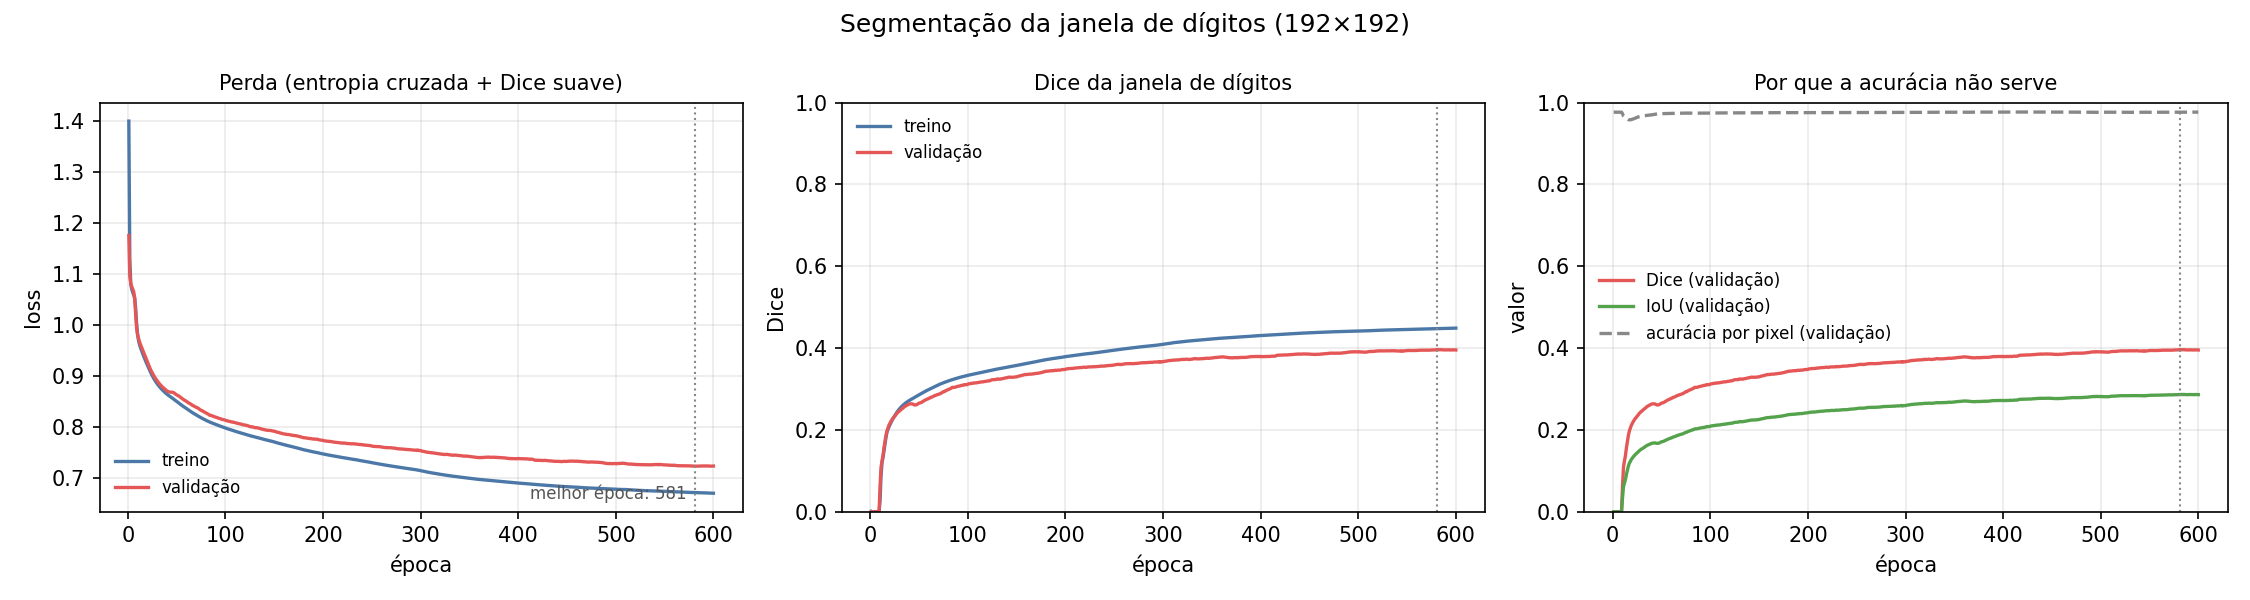
\includegraphics[width=\textwidth]{sections/imagens/ocr_treino_segmentacao.png}
    \legend{Fonte: Elaborado pelos autores (2026).}
\end{figure}

No conjunto de teste, com 186 fotos não vistas no treino, o modelo em INT8 obteve Dice de
0,39 e IoU de 0,28. O resultado é fraco. A acurácia por pixel supera 98\%, mas não serve
como medida, pois o fundo domina a imagem, como mostra o terceiro gráfico da
Figura~\ref{fig:treino_segmentacao}. As curvas de treino e validação próximas indicam
subajuste: a rede, minúscula e sem conexões de salto, não tem capacidade para localizar a
janela com precisão.

No uso, a caixa da janela é o menor retângulo que contém os pixels marcados pela máscara,
convertido para as coordenadas do quadro de $160 \times 120$ pixels. Como a máscara
prevista transborda a janela, essa caixa fica muito maior do que deveria. Nas fotos do
conjunto de teste comum, descrito adiante, a caixa prevista
teve mediana de $125 \times 85$ pixels, cobrindo quase todo o mostrador, enquanto a janela
real mede cerca de $97 \times 18$ pixels. Com essa caixa, cada fatia contém pedaços de
vários roletes e do mostrador, e a leitura falha.

\subsubsection{Classificador de dígitos}
\label{subsubsec:classificador}

O classificador recebe a imagem de um único rolete, redimensionada para $28 \times 28$
pixels em tons de cinza, e devolve a probabilidade de cada um dos dez dígitos. É uma rede
neural convolucional com 72.442 parâmetros, cuja arquitetura é apresentada na
Tabela~\ref{tab:arquitetura_classificador}. Quantizado em INT8, o modelo ocupa 81,5~KB.

\begin{table}[H]
    \centering
    \caption{Arquitetura do classificador de dígitos}
    \label{tab:arquitetura_classificador}
    \begin{tabular}{@{}lll@{}}
        \toprule
        \textbf{Camada} & \textbf{Configuração} & \textbf{Saída} \\
        \midrule
        Entrada & imagem em tons de cinza & $28 \times 28 \times 1$ \\
        Convolução $\times 2$ & 16 filtros $3 \times 3$, ReLU & $28 \times 28 \times 16$ \\
        \textit{Max pooling} & $2 \times 2$ & $14 \times 14 \times 16$ \\
        Convolução $\times 2$ & 32 filtros $3 \times 3$, ReLU & $14 \times 14 \times 32$ \\
        \textit{Max pooling} & $2 \times 2$ & $7 \times 7 \times 32$ \\
        Convolução & 64 filtros $3 \times 3$, ReLU & $7 \times 7 \times 64$ \\
        \textit{Max pooling} & $2 \times 2$ & $3 \times 3 \times 64$ \\
        Achatamento & --- & 576 \\
        Densa & 64 neurônios, ReLU, \textit{dropout} de 30\% & 64 \\
        Densa (saída) & 10 neurônios, \textit{softmax} & 10 \\
        \bottomrule
    \end{tabular}
    \legend{Fonte: Elaborado pelos autores (2026).}
\end{table}

O treinamento foi feito em duas fases. Na fase A, o modelo foi treinado com os recortes dos
dois conjuntos públicos, com o otimizador Adam (taxa de aprendizado de $5 \times 10^{-4}$),
lotes de 128 recortes e pesos por classe para compensar o excesso de zeros. Para aproximar
os recortes das imagens do \gls{esp32cam}, foi aplicado aumento de dados com redução e
ampliação da resolução, ruído gaussiano, pequenas rotações e translações e variação de
contraste. O treino foi interrompido por parada antecipada após 37 épocas, com a melhor
época na 27.ª, e atingiu 94,65\% de acurácia na validação
(Figura~\ref{fig:treino_classificador}).

\begin{figure}[H]
    \centering
    \caption{Evolução do treino do classificador de dígitos (fase A)}
    \label{fig:treino_classificador}
    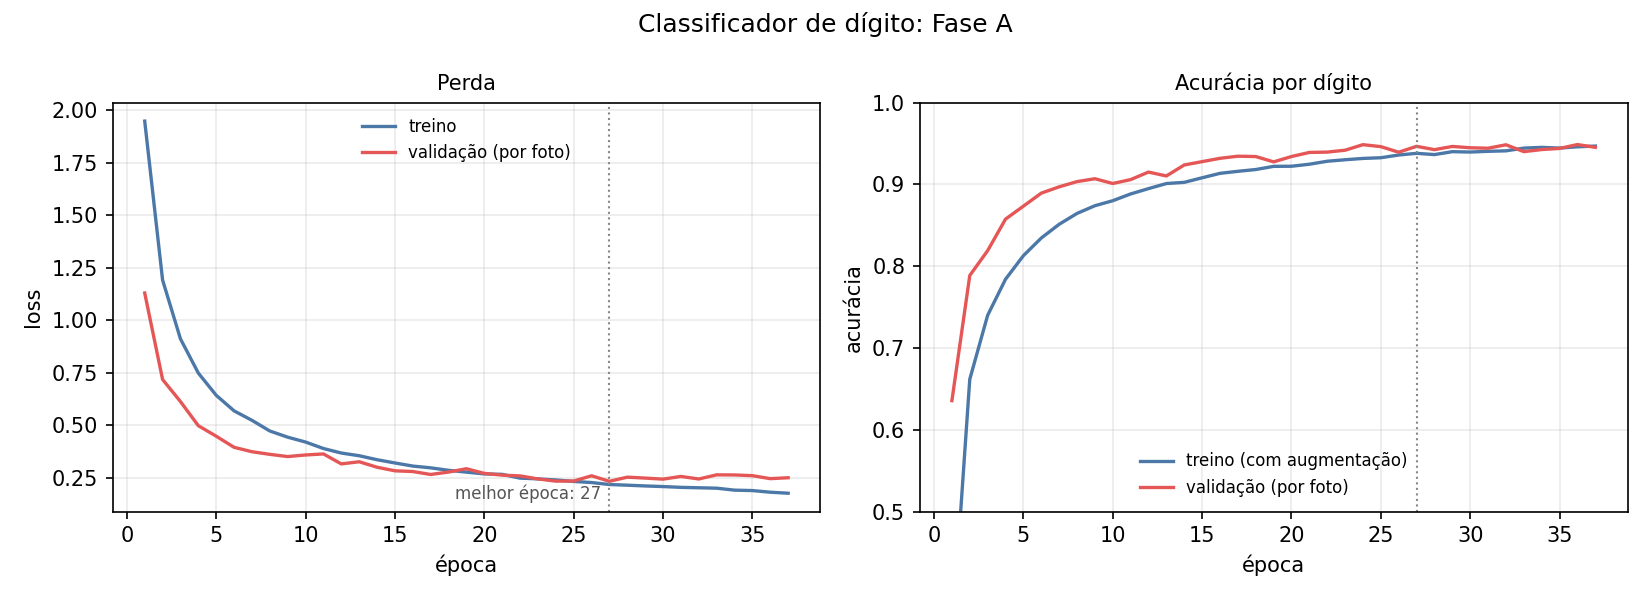
\includegraphics[width=\textwidth]{sections/imagens/ocr_treino_classificador.png}
    \legend{Fonte: Elaborado pelos autores (2026).}
\end{figure}

Na fase B, o modelo passou por um ajuste fino de cinco épocas, com taxa de aprendizado dez
vezes menor ($5 \times 10^{-5}$), usando os 24 recortes do \gls{esp32cam}, fortemente
aumentados e repetidos, junto com uma parte dos recortes da fase A, para que o modelo não
esquecesse o que já havia aprendido. Ao final, a acurácia de validação do modelo em ponto
flutuante foi de 95,46\%.

\subsubsection{Quantização e exportação}
\label{subsubsec:quantizacao_ocr}

Os dois modelos foram quantizados em INT8 após o treinamento (\textit{post-training
quantization}), com um conjunto representativo de imagens para calibrar as escalas. A
quantização foi completa: pesos, ativações, entrada e saída em inteiros de 8 bits, usando
apenas operadores INT8 do TensorFlow Lite. Na entrada, a escala de $1/255$ com ponto zero
de $-128$ permite converter cada pixel diretamente, subtraindo 128 do seu valor. Diferente
do pipeline A, que usou treinamento consciente da quantização (QAT), o pipeline B não
precisou dessa técnica: a perda de acurácia na quantização foi desprezível, como mostra a
avaliação da hipótese H1 nos resultados. Por fim, cada modelo \texttt{.tflite} foi
convertido em um vetor de bytes em um arquivo de cabeçalho C (\texttt{.h}), incluído no
firmware.

\subsubsection{Leitura com janela calibrada na instalação}
\label{subsubsec:leitura_roi}

Dada a caixa da janela, a leitura é feita da mesma forma no firmware e no servidor: a
caixa é dividida em $N$ fatias de largura igual, uma por rolete; cada fatia é
redimensionada para $28 \times 28$ pixels por vizinho mais próximo, convertida para INT8 e
classificada; e os dígitos de maior probabilidade são concatenados na leitura. O número
$N$ de roletes é um parâmetro configurado por medidor: seis no medidor usado nos testes de
hardware.

Como o modelo de localização não encontra a janela com precisão, os resultados com a caixa
prevista por ele são próximos de zero. Esses resultados \textbf{não refletem a capacidade
de leitura do classificador}, e sim o erro da localização: com a caixa errada, as fatias
não correspondem aos roletes. Quando a janela é informada corretamente, o mesmo
classificador lê os dígitos com alta acurácia. A Figura~\ref{fig:leitura_caixa_manual}
mostra cinco capturas do \gls{esp32cam} em que a janela foi marcada à mão: todas as cinco
leituras e os 26 dígitos foram reconhecidos corretamente.

\begin{figure}[htbp]
    \centering
    \caption{Leitura com a janela de dígitos marcada manualmente em cinco capturas do
    \gls{esp32cam}}
    \label{fig:leitura_caixa_manual}
    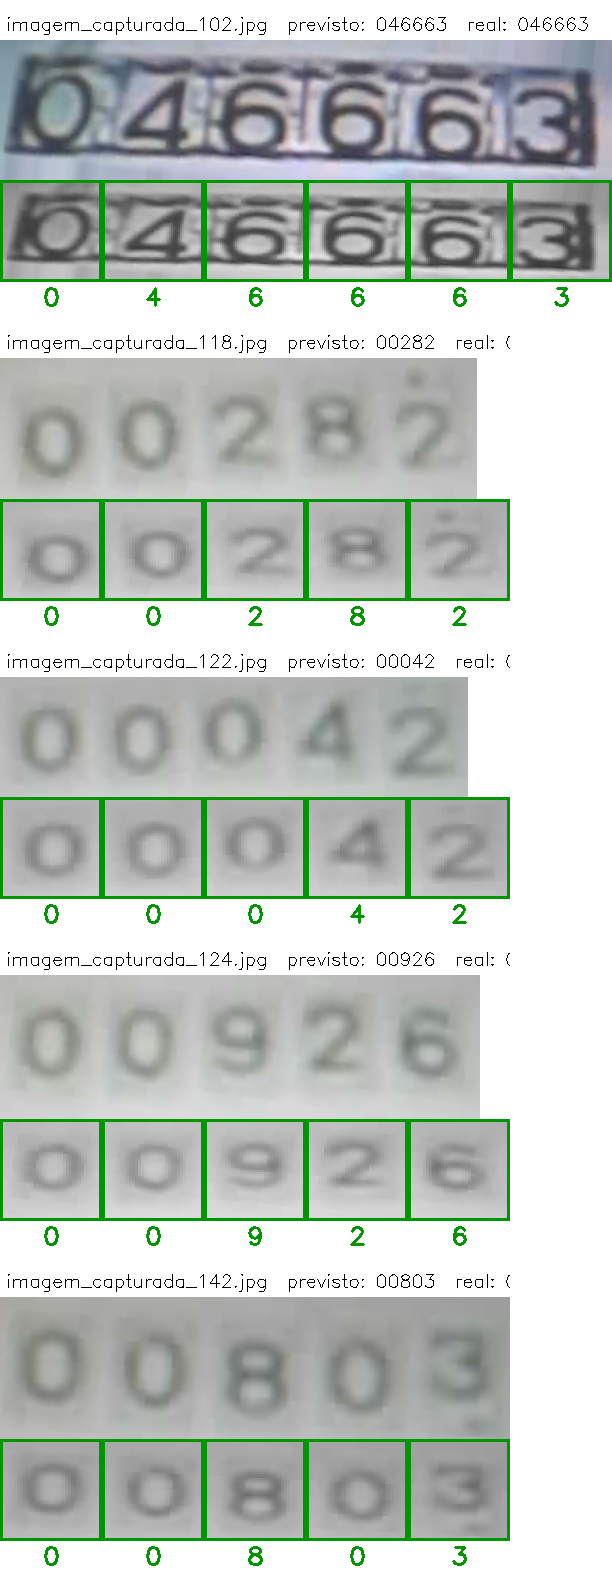
\includegraphics[height=0.55\textheight]{sections/imagens/ocr_leitura_caixa_manual.png}
    \legend{Fonte: Elaborado pelos autores (2026). Em cada captura, a faixa superior é a
    janela recortada, a inferior mostra as fatias e, abaixo, o dígito previsto para cada
    uma.}
\end{figure}

Por isso, a solução adotada dispensa a localização automática. Em uma instalação real, a
câmera fica fixa diante do medidor, de modo que a janela de dígitos ocupa sempre a mesma
região do quadro. Assim, a região de interesse (ROI) e a inclinação dos roletes são
calibradas uma única vez, na instalação, e usadas em todas as leituras seguintes. Essa
calibração precisa ser precisa: a avaliação apresentada nos resultados indica que a ROI
deve estar a cerca de um ou dois pixels da posição correta no quadro de
$160 \times 120$ pixels, em que cada dígito tem aproximadamente 16 pixels de largura.

Nas medições de latência e consumo em hardware, o firmware de borda ainda executava o
modelo de localização a cada leitura, com a câmera posicionada à mão para que a janela
ocupasse a maior parte do quadro e a caixa prevista ficasse próxima dela. Essa configuração é descrita na próxima seção, e o efeito
de remover a localização é discutido nos resultados.

\subsection{Firmware do nó sensor}
\label{subsec:firmware}

Os dois firmwares do nó, um para cada fluxo, foram escritos para o \gls{esp32cam} com o
\textit{core} Arduino-ESP32 3.0.7 e compartilham a mesma estrutura: configuração da câmera,
comunicação com o módulo de rádio, modo autônomo com \textit{deep sleep} e registro dos
tempos de cada etapa. Além do modo autônomo, ambos aceitam comandos pela porta serial,
usados nos testes e nas medições: disparo de uma leitura, ativação e desativação do modo
autônomo, \textit{deep sleep} avulso e repasse de comandos AT ao módulo de rádio.

\subsubsection{Ciclo de operação}
\label{subsubsec:ciclo_operacao}

No modo autônomo, o nó executa ciclos de leitura separados por períodos de
\textit{deep sleep}. Ao despertar pelo temporizador, o microcontrolador reinicia, configura
a câmera em tons de cinza na resolução de $160 \times 120$ pixels, captura um quadro e,
logo em seguida, desliga a câmera, pois ela não é necessária no restante do ciclo. A
partir desse ponto, cada fluxo segue um caminho, como resume a
Tabela~\ref{tab:ciclo_fluxos}.

\begin{table}[H]
    \centering
    \caption{Etapas de um ciclo de leitura em cada fluxo}
    \label{tab:ciclo_fluxos}
    \begin{tabularx}{\textwidth}{@{}lXX@{}}
        \toprule
        \textbf{Etapa} & \textbf{Fluxo em nuvem} & \textbf{Fluxo em borda} \\
        \midrule
        Despertar & \multicolumn{2}{l}{Reinício pelo temporizador e configuração da câmera} \\
        Captura & \multicolumn{2}{l}{Quadro de $160 \times 120$ pixels em cinza; câmera desligada em seguida} \\
        Processamento & Compressão JPEG e divisão em blocos de 175~bytes & Localização da janela
        e classificação dos dígitos com TensorFlow Lite Micro \\
        Envio & Um \textit{uplink} por bloco, com 7~s de intervalo (19 a 27 blocos) & Um único
        \textit{uplink} de 9~bytes \\
        Registro & \multicolumn{2}{l}{Linha de fim de ciclo na serial, com os tempos de cada etapa} \\
        Repouso & \multicolumn{2}{l}{\textit{Deep sleep} até o próximo ciclo} \\
        \bottomrule
    \end{tabularx}
    \legend{Fonte: Elaborado pelos autores (2026).}
\end{table}

Ao fim de cada ciclo, o firmware escreve na serial uma linha padronizada com o número do
ciclo, o resultado do envio e a duração de cada etapa (captura, processamento e envio).
Essa linha é lida pelos \textit{scripts} de medição, o que permite comparar os dois fluxos
com as mesmas ferramentas.

Antes de entrar em \textit{deep sleep}, o firmware desativa o driver da câmera, coloca o
sensor em modo de baixo consumo pelo pino de \textit{power-down} (GPIO~32), apaga o LED
de \textit{flash} (GPIO~4) e mantém o nível desses pinos durante o repouso. O contador de
ciclos e o estado do modo autônomo ficam na memória RTC, que é preservada durante o
\textit{deep sleep}. Apenas o ESP32 é colocado em repouso: o módulo Radioenge continua
alimentado e não recebe comando para entrar em modo suspenso, o que mantém nele a sessão
\gls{lorawan} e o contador de quadros, mas também mantém o seu consumo durante o repouso,
como discutido nos resultados. Nas medições, o intervalo de \textit{deep sleep} foi de
30~s nos dois fluxos.

\subsubsection{Execução dos modelos no microcontrolador}
\label{subsubsec:tflm}

No fluxo em borda, os modelos são executados com o TensorFlow Lite Micro, na versão
\texttt{esp-tflite-micro} 1.3.1 com a biblioteca de otimização \texttt{esp-nn} 1.1.0, ambas
incluídas no \textit{core} 3.0.7. Os dois modelos \texttt{.tflite} ficam na memória
\textit{flash} como vetores de bytes, e cada um tem o seu próprio interpretador, criado com
um registro de operadores que contém apenas os operadores usados pelo modelo: sete na
localização da janela e oito no classificador. O firmware compilado ocupa 563~KB, cerca de
17\% da memória de programa.

O TensorFlow Lite Micro não aloca memória dinamicamente: cada interpretador recebe uma
área de trabalho (\textit{arena}) de tamanho fixo, onde ficam os tensores intermediários.
As duas \textit{arenas} foram alocadas na PSRAM de 4~MB da placa. A
Tabela~\ref{tab:memoria_tflm} mostra a memória reservada e a efetivamente usada, medida na
placa durante 61 capturas.

\begin{table}[H]
    \centering
    \caption{Uso da PSRAM pelo fluxo em borda}
    \label{tab:memoria_tflm}
    \begin{tabular}{@{}lrr@{}}
        \toprule
        \textbf{Item} & \textbf{Reservado (bytes)} & \textbf{Usado (bytes)} \\
        \midrule
        Buffer de quadro da câmera & --- & $\approx$19.216 \\
        \textit{Arena} da localização da janela & 2.097.152 & 1.623.852 \\
        \textit{Arena} do classificador de dígitos & 786.432 & 28.556 \\
        PSRAM livre após as alocações & \multicolumn{2}{r}{1.289.292} \\
        \bottomrule
    \end{tabular}
    \legend{Fonte: Elaborado pelos autores (2026).}
\end{table}

O dimensionamento das \textit{arenas} exigiu ajustes durante os testes em placa. A
primeira estimativa, baseada no maior tensor intermediário do modelo de localização,
reservou 1~MB, e a alocação falhou: o interpretador mantém vários tensores intermediários
ativos ao mesmo tempo, e o modelo precisou de cerca de 1,6~MB. A \textit{arena} foi então
ampliada para 2~MB. A \textit{arena} do classificador, de 768~KB, mostrou-se
superdimensionada, pois o modelo usa menos de 29~KB. Para evitar novas tentativas na
placa, foi escrito um \textit{script} que reproduz o planejador de memória do
TensorFlow Lite Micro a partir do arquivo \texttt{.tflite}; para o modelo de localização,
ele estimou 1.622.016~bytes, contra 1.623.852~bytes medidos. Esse mesmo \textit{script}
confirmou que o modelo de localização do pipeline A, que pediu 15,3~MB, não caberia na
placa.

A leitura no firmware segue os passos descritos na
Seção~\ref{subsubsec:leitura_roi}. O quadro capturado é copiado para um buffer próprio e a
câmera é desligada antes da inferência. Para o modelo de localização, o quadro é
redimensionado por vizinho mais próximo para $192 \times 192$ pixels diretamente no
tensor de entrada, já convertido para INT8 pela subtração de 128 de cada pixel. Na saída,
os valores INT8 maiores que zero, que correspondem a probabilidade superior a 0,5, formam
a máscara, e a caixa é o menor retângulo que a contém. Cada uma das $N$ fatias da caixa é
redimensionada para $28 \times 28$ pixels e classificada, e o dígito de maior pontuação é
escrito na leitura. Se a máscara vier vazia, a leitura é enviada com traços no lugar dos
dígitos.

O tempo de inferência medido na placa foi muito maior do que o esperado para modelos tão
pequenos. Em 61 capturas, a localização da janela levou mediana de 15.564~ms, com variação
de apenas 4~ms entre capturas, e a classificação dos seis dígitos levou 1.995~ms, para um
total de 17.838~ms por leitura. A causa não foi investigada; uma hipótese é que parte dos
operadores do modelo de localização, como a convolução transposta, não tenha versão
otimizada na \texttt{esp-nn} e seja executada pelas implementações de referência, em C
genérico. Durante essas capturas, a temperatura interna do chip permaneceu entre 72 e
74~°C.

Como discutido na Seção~\ref{subsubsec:leitura_roi}, a solução adotada dispensa o modelo de
localização e usa uma ROI calibrada na instalação. O firmware usado nas medições, porém,
ainda executa a localização a cada leitura; a versão com ROI fixa não foi implementada.
Sem a localização, a leitura no nó ficaria restrita à classificação dos dígitos, de cerca
de 2~s, o que é uma estimativa, e não uma medição.

\subsubsection{Firmware de depuração e calibração}
\label{subsubsec:firmware_debug}

Um terceiro firmware, sem rádio, foi usado para posicionar a câmera diante do medidor e
para medir o desempenho dos modelos na placa. A cada 5~s, ele captura um quadro, executa a
leitura completa, desenha sobre a imagem a caixa encontrada e as divisões das fatias e
envia ao computador a imagem anotada, a leitura e métricas de memória, tempo e
temperatura. Um \textit{script} no computador grava as imagens e as métricas em arquivo.
Com ele, a câmera foi ajustada à mão até que a janela de dígitos ocupasse o quadro e a
caixa prevista coincidisse com ela; a partir desse ponto, a leitura do medidor de teste se
estabilizou. Os dados de memória e de tempo de inferência apresentados nesta seção vêm
desse firmware.

\subsection{Servidor da aplicação}
\label{subsec:servidor}

No servidor, a recepção é feita pelo \textit{script} \texttt{reconstrutor.py}, descrito na
Seção~\ref{subsubsec:recepcao}: no fluxo em borda, a leitura chega pronta na porta~2; no
fluxo em nuvem, a imagem remontada é gravada em disco. O \gls{ocr} do fluxo em nuvem é
executado sobre essas imagens pelo \textit{script} \texttt{pipeline\_nuvem.py}.

Para que a única diferença entre os fluxos seja o local do processamento, o servidor
executa os mesmos arquivos \texttt{.tflite} INT8 do firmware, com o interpretador LiteRT
2.3.0, e reproduz a mesma lógica: o mesmo redimensionamento por vizinho mais próximo, com
o mesmo cálculo de índices, a mesma conversão para INT8, o mesmo limiar na máscara e o
mesmo fatiamento. O acelerador XNNPACK do LiteRT foi desativado, para que os operadores
sejam executados pelas implementações de referência, como no microcontrolador. A única
diferença no dado de entrada é a compressão JPEG com qualidade 90, que o fluxo em borda não
sofre.

\subsubsection{Tempo de inferência no servidor}
\label{subsubsec:tempo_servidor}

Na implementação atual, o \gls{ocr} do servidor não é disparado automaticamente quando a
imagem fica completa: ele é executado depois, sobre as imagens gravadas. Por isso, a
latência medida no fluxo em nuvem termina no momento em que a imagem fica disponível no
servidor, e o tempo de inferência foi medido à parte. Em um computador com processador
AMD Ryzen 5 5600GT, as 21 imagens completas recebidas pelo enlace foram lidas cinco vezes
cada. A Tabela~\ref{tab:tempo_inferencia} compara os tempos com os do microcontrolador.

\begin{table}[H]
    \centering
    \caption{Tempo de inferência por leitura no nó e no servidor (mediana)}
    \label{tab:tempo_inferencia}
    \begin{tabular}{@{}lrr@{}}
        \toprule
        \textbf{Etapa} & \textbf{\gls{esp32cam} (ms)} & \textbf{Servidor (ms)} \\
        \midrule
        Localização da janela & 15.564 & 4,30 \\
        Leitura completa (localização e seis dígitos) & 17.838 & 6,25 \\
        Leitura com ROI fixa (só os seis dígitos) & $\approx$1.995 & 1,91 \\
        \bottomrule
    \end{tabular}
    \legend{Fonte: Elaborado pelos autores (2026). No servidor, os tempos incluem a
    decodificação do JPEG; no \gls{esp32cam}, a leitura com ROI fixa corresponde ao tempo
    medido da classificação dos dígitos.}
\end{table}

O servidor executa a leitura completa cerca de 2.800 vezes mais rápido que o
microcontrolador. Diante da latência de envio da imagem, de mais de dois minutos, o tempo
de inferência no servidor é desprezível, e a omissão dessa etapa na latência medida não
altera a comparação entre os fluxos.

\subsubsection{Recursos disponíveis apenas no servidor}
\label{subsubsec:recursos_servidor}

O baixo custo da inferência no servidor permite etapas que seriam caras no
microcontrolador. Duas foram implementadas e avaliadas:

\begin{itemize}
    \item \textbf{Correção da inclinação}: a fileira de roletes costuma aparecer levemente
    inclinada no quadro. O servidor detecta as bordas da imagem (Canny), extrai os segmentos
    de reta pela transformada de Hough, toma a mediana ponderada pelo comprimento dos
    ângulos dos segmentos quase horizontais (até $\pm 20^\circ$) e gira o quadro para
    endireitá-lo antes da leitura.
    \item \textbf{Votação entre caixas deslocadas}: para tolerar pequenos erros na posição
    da ROI, o classificador é aplicado a cinco versões da caixa, a original e outras quatro
    deslocadas de 2~pixels na horizontal e de 1~pixel na vertical, e as pontuações de cada
    fatia são somadas antes da escolha do dígito. No microcontrolador, isso multiplicaria
    por cinco os cerca de 2~s da classificação.
\end{itemize}

A ROI é informada ao servidor como um retângulo em coordenadas do quadro de
$160 \times 120$ pixels e é calibrada uma vez por instalação. Para isso, um
\textit{script} auxiliar desenha uma grade de coordenadas sobre o quadro ampliado, a
partir da qual a janela é lida à mão. Ainda não existe uma ferramenta que faça essa
calibração de forma automática ou guiada, o que é uma limitação da solução atual. O efeito
da correção da inclinação, da votação e da precisão da ROI sobre a acurácia é apresentado
nos resultados.


\section{Experimentos e cenário de testes}
\label{sec:experimentos}
Os experimentos foram planejados para responder às três hipóteses da
Seção~\ref{subsec:hipotese}. A Tabela~\ref{tab:plano_experimentos} relaciona cada
experimento à hipótese avaliada, aos dados utilizados e às métricas principais. Os
experimentos de reconhecimento foram executados no computador, sobre conjuntos de imagens
fixos e versionados no repositório. Os de latência, entrega e consumo foram executados com
o protótipo em bancada, com os firmwares dos dois fluxos descritos na
Seção~\ref{subsec:firmware}.

\begin{table}[H]
    \centering
    \caption{Plano de experimentação}
    \label{tab:plano_experimentos}
    \begin{tabularx}{\textwidth}{@{}>{\raggedright\arraybackslash}p{3.1cm}c>{\raggedright\arraybackslash}X>{\raggedright\arraybackslash}p{3.6cm}@{}}
        \toprule
        \textbf{Experimento} & \textbf{Hipótese} & \textbf{Dados e condição} & \textbf{Métricas} \\
        \midrule
        Efeito da quantização & H1 & Mesmo classificador em ponto flutuante e em INT8; 7.378
        recortes de validação e 1.894 imagens de teste independentes & Acurácia por recorte,
        leitura exata, acurácia por dígito, CER \\
        \addlinespace
        Leitura de ponta a ponta & --- & 39 fotos do conjunto de teste comum e 21 fotos de
        hidrômetros físicos; janela prevista pelo modelo e janela marcada à mão & Leitura exata,
        acurácia por dígito, CER, Dice e IoU \\
        \addlinespace
        Latência e entrega & H2 & Nó em ciclo autônomo com \textit{deep sleep}: 30 leituras no
        fluxo em nuvem e 34 no fluxo em borda; 30 envios adicionais de imagem com o nó sempre
        ligado & Latência ponta a ponta, \gls{pdr} por pacote, taxa de entrega por leitura \\
        \addlinespace
        Consumo de energia & H3 & Corrente do nó medida em 30 ciclos do fluxo em nuvem e 32
        do fluxo em borda & Carga por leitura (mAh), corrente acordado e em repouso, autonomia
        estimada \\
        \bottomrule
    \end{tabularx}
    \legend{Fonte: Elaborado pelos autores (2026).}
\end{table}

Como os dois fluxos usam os mesmos modelos INT8 e a mesma lógica de leitura
(Seção~\ref{subsec:visao_geral}), a acurácia do reconhecimento não é uma variável entre
eles. Por isso, a hipótese H1 é avaliada pela comparação entre as versões em ponto
flutuante e em INT8 do mesmo modelo, e não entre os fluxos. Já nos experimentos das
hipóteses H2 e H3, a única variável é o fluxo: o hardware, o enlace, o intervalo de repouso
e a bancada são os mesmos.

\subsection{Métricas}
\label{subsec:metricas_experimentos}

\subsubsection{Reconhecimento}
\label{subsubsec:metricas_ocr}

Para cada imagem, a leitura prevista $\hat{y}$ é comparada com a
leitura real $y$, ambas sequências de $N$ dígitos. São usadas três métricas sobre um
conjunto de $M$ imagens: a taxa de leitura exata, que conta apenas as leituras com todos os
dígitos corretos; a acurácia por dígito, que compara posição a posição; e a taxa de erro de
caracteres (\textit{character error rate}, CER), baseada na distância de edição de
Levenshtein $d_{\mathrm{L}}$, isto é, o número mínimo de inserções, remoções e substituições
que transformam uma sequência na outra:

\begin{equation}
    \label{eq:leitura_exata}
    Acc_{\mathrm{leitura}} = \frac{1}{M}\sum_{m=1}^{M} \mathbf{1}\!\left[\hat{y}_m = y_m\right]
    \qquad
    Acc_{\textrm{dígito}} = \frac{\sum_{m}\sum_{k=1}^{N_m} \mathbf{1}\!\left[\hat{y}_{m,k} = y_{m,k}\right]}{\sum_{m} N_m}
\end{equation}

\begin{equation}
    \label{eq:cer}
    CER = \frac{\sum_{m} d_{\mathrm{L}}(\hat{y}_m, y_m)}{\sum_{m} N_m}
\end{equation}

A taxa de leitura exata é a métrica mais exigente e a que interessa à aplicação: uma
leitura com um único dígito errado é uma leitura errada. Para o classificador isolado, a
métrica é a acurácia por recorte, a fração de recortes de um único dígito classificados
corretamente, acompanhada da acurácia por classe e da matriz de confusão.

A qualidade da localização da janela é medida pela sobreposição entre a máscara prevista
$P$ e a máscara de referência $G$, pelos coeficientes Dice e IoU (\textit{intersection over
union}):

\begin{equation}
    \label{eq:dice_iou}
    Dice = \frac{2\,|P \cap G|}{|P| + |G|}
    \qquad
    IoU = \frac{|P \cap G|}{|P \cup G|}
\end{equation}

\subsubsection{Latência e entrega}
\label{subsubsec:metricas_latencia}

A latência ponta a ponta de uma leitura é o intervalo entre
o disparo no nó e o instante em que o dado fica disponível no servidor: a imagem remontada,
no fluxo em nuvem, ou a leitura decodificada, no fluxo em borda. A entrega é avaliada de
duas formas. A primeira é o \gls{pdr} por pacote, definido na Equação~\eqref{eq:pdr}. A
segunda é a taxa de entrega por leitura, a fração das leituras disparadas cujo dado chegou
completo ao servidor:

\begin{equation}
    \label{eq:entrega_leitura}
    E_{\mathrm{leitura}} = \frac{\text{leituras disponíveis no servidor}}{\text{leituras disparadas}}
\end{equation}

As duas métricas diferem no fluxo em nuvem: como nenhum dos firmwares retransmite blocos no
modo autônomo, uma imagem com um único bloco perdido não é remontada, e a leitura se perde
mesmo com um \gls{pdr} alto. No fluxo em borda, em que cada leitura ocupa um pacote, as duas
coincidem. As taxas de entrega por leitura dos dois fluxos são comparadas pelo teste exato
de Fisher, adequado a proporções com amostras pequenas.

\subsubsection{Energia}
\label{subsubsec:metricas_energia}

A carga consumida em uma leitura é a integral da corrente $i(t)$ ao
longo de um ciclo completo, de um despertar ao seguinte, incluindo o repouso, calculada pela
regra do trapézio sobre as amostras e expressa em mAh:

\begin{equation}
    \label{eq:carga_leitura}
    Q_{\mathrm{leitura}} = \frac{1}{3600}\int_{t_{\mathrm{despertar},k}}^{t_{\mathrm{despertar},k+1}} i(t)\,dt
\end{equation}

\noindent com $i$ em mA e $t$ em segundos. Para estimar a autonomia em outros intervalos
entre leituras, o ciclo é modelado por dois estados: acordado, com corrente média
$I_{\mathrm{ac}}$ durante $t_{\mathrm{ac}}$, e em repouso, com corrente $I_{\mathrm{rep}}$
no restante do intervalo $T$. A autonomia $A$, em dias, para uma bateria de capacidade
$C_{\mathrm{bat}}$ em mAh, é então:

\begin{equation}
    \label{eq:autonomia_modelo}
    Q_{\mathrm{leitura}}(T) = \frac{I_{\mathrm{ac}}\,t_{\mathrm{ac}} + I_{\mathrm{rep}}\,(T - t_{\mathrm{ac}})}{3600}
    \qquad
    A = \frac{C_{\mathrm{bat}}}{Q_{\mathrm{leitura}}(T)} \cdot \frac{T}{86400}
\end{equation}

O modelo é ideal: não considera as perdas do regulador, a autodescarga nem a variação da
capacidade da bateria com a temperatura, de modo que a autonomia calculada é um limite
superior.

\subsection{Cenário de bancada}
\label{subsec:bancada}

Todas as medições em hardware foram feitas em 27 de outubro de 2026, em bancada, com o nó
sensor e o receptor a cerca de 2~m de distância. Nessa condição, o RSSI médio dos quadros
recebidos ficou entre $-34$ e $-27$~dBm, um sinal muito forte. Como antecipado na
Seção~\ref{subsec:simplificacoes}, o cenário avalia o comportamento dos fluxos, e não o
alcance do enlace. O enlace usou a configuração da Tabela~\ref{tab:parametros_enlace} nos
dois fluxos, e a câmera ficou fixa, apontada para o mostrador de um hidrômetro.

Nos experimentos de latência, entrega e consumo, os dois firmwares operaram no modo
autônomo com repouso de 30~s (\texttt{AUTO:30}), descrito na
Seção~\ref{subsubsec:ciclo_operacao}, e sem a janela para receber o comando de parada após
o despertar. O intervalo de 30~s não representa uma instalação real, em que as leituras
seriam espaçadas de minutos ou horas; ele foi escolhido para obter pelo menos 30 ciclos de
cada fluxo em poucas horas de medição. O efeito de intervalos mais longos é obtido pelo
modelo da Equação~\eqref{eq:autonomia_modelo}.

O nó foi alimentado pelos 5~V da porta USB da placa de gravação ESP32-CAM-MB, que também
fornecia a serial usada para acompanhar o log do firmware. O computador lia ao mesmo tempo
a serial do nó e a do receptor, de modo que todos os instantes foram marcados por um único
relógio, o do computador. A incerteza desses instantes, de alguns milissegundos, é
desprezível diante das latências medidas.

\subsection{Avaliação do reconhecimento}
\label{subsec:exp_ocr}

\subsubsection{Efeito da quantização (H1)}
\label{subsubsec:exp_quantizacao}

O classificador de dígitos treinado (Seção~\ref{subsubsec:classificador}) foi salvo em
ponto flutuante de 32 bits e, após a quantização (Seção~\ref{subsubsec:quantizacao_ocr}),
em INT8. As duas versões foram avaliadas sobre os mesmos 7.378 recortes de validação, da
divisão por foto descrita na Seção~\ref{subsubsec:dados_ocr}, por um \textit{script} que
apenas carrega os modelos já treinados e mede, sem treinar novamente. Como os pesos de
origem e os dados são os mesmos, a diferença de acurácia entre as versões isola o efeito
da quantização.

Como os recortes de validação vêm das mesmas fontes usadas no treino, o modelo INT8 também
foi avaliado nas pastas de teste do \textit{Word-Wheel Water Meter Dataset}, que ficaram
fora de todo o treinamento: 1.894 imagens da janela de dígitos, de $200 \times 60$ pixels.
Cada imagem foi dividida em $N$ fatias iguais, como no firmware, e cada fatia foi
classificada. Como essas imagens já são recortes retos da janela, esse teste mede o
classificador e o fatiamento, sem a etapa de localização. O teste foi repetido com o modelo
ao fim da fase A e com o modelo final, após o ajuste fino da fase B, para verificar se o
ajuste às imagens do \gls{esp32cam} prejudicou a generalização.

\subsubsection{Leitura de ponta a ponta}
\label{subsubsec:exp_leitura}

Para avaliar o pipeline completo, da imagem da câmera até a leitura, foram usados dois
conjuntos de fotos capturadas pelo \gls{esp32cam}, nenhum deles usado no treino ou no
ajuste dos modelos.

O \textbf{conjunto de teste comum} reúne 39 fotos de um monitor que exibia imagens de
hidrômetros, com 19 leituras distintas de dois modelos de medidor, um de cinco e outro de
seis roletes. As fotos foram selecionadas entre 152 capturas, com dois critérios: sem
rotação de 90° ou 180° e sem nenhum rolete parado entre dois números, caso em que a
leitura real é ambígua. Por comparação de \textit{hash}, verificou-se que nenhuma delas é
idêntica às fotos usadas no treino. O gabarito de cada foto foi conferido manualmente,
sobre uma folha que imprime a leitura esperada sobre a imagem, e para cada foto também foi
marcada à mão a janela de dígitos.

O \textbf{conjunto de hidrômetros físicos} reúne 21 fotos de medidores reais, de
diferentes modelos, com cinco a oito roletes, capturadas pelo \gls{esp32cam} no quadro de
$160 \times 120$ pixels. Ao contrário do conjunto comum, essas fotos têm reflexos no vidro,
iluminação variada e ângulos diversos. A leitura de cada foto foi anotada manualmente. Para
cada foto, foram marcados também a inclinação da fileira de roletes, a janela de dígitos no
quadro endireitado e a polaridade da janela: dígitos escuros em fundo claro ou dígitos
claros em fundo escuro. A inclinação foi a estimada pela transformada de Hough quando ela
deixava a fileira reta, em 16 fotos, e corrigida à mão nas outras cinco. A janela foi marcada
pela geometria da imagem, sobre o quadro ampliado com uma grade de coordenadas, a partir das
bordas da janela e dos centros dos roletes, de modo que as divisões das fatias caíssem entre
eles. Todas as marcações foram concluídas antes da execução da leitura e não foram ajustadas
pelo resultado.

Cada foto foi avaliada nos dois fluxos. No fluxo em borda, o quadro de
$160 \times 120$ pixels é lido diretamente; no fluxo em nuvem, o mesmo quadro é antes
codificado em JPEG com qualidade 90 e decodificado, como ocorre na transmissão. Essa
avaliação é uma emulação em Python, com os mesmos arquivos \texttt{.tflite} INT8, e não a
execução na placa. No conjunto comum, as fotos foram lidas em três configurações:

\begin{enumerate}
    \item \textbf{Janela prevista pelo modelo}: o pipeline completo, como no firmware, com
    a caixa obtida da máscara do modelo de localização.
    \item \textbf{Janela marcada à mão}: a caixa é informada diretamente e o modelo de
    localização não é usado. Essa configuração corresponde à ROI calibrada na instalação
    (Seção~\ref{subsubsec:leitura_roi}) e mede o classificador e o fatiamento quando a
    janela está correta.
    \item \textbf{Janela marcada à mão com correção de inclinação}: o quadro é antes
    endireitado no servidor pelo ângulo estimado com a transformada de Hough, recurso
    disponível apenas no fluxo em nuvem (Seção~\ref{subsubsec:recursos_servidor}).
\end{enumerate}

A distinção entre essas configurações é essencial para interpretar os resultados.
Quando a janela é prevista pelo modelo, o erro da leitura é dominado pelo erro da
localização: com uma caixa que cobre quase todo o mostrador, as fatias não correspondem
aos roletes, e nenhum classificador acertaria a leitura. Assim, os resultados da primeira
configuração medem o modelo de localização, e não a capacidade de leitura do classificador,
que é medida pelas configurações com a janela marcada à mão.

O conjunto de hidrômetros físicos, cujas fotos têm inclinações de até cerca de 55°, foi lido
com a janela prevista pelo modelo e com a janela e a inclinação marcadas à mão. Nesse caso,
a rotação do quadro foi aplicada nos dois fluxos, o que no firmware exigiria uma rotação com
ângulo fixo, ainda não implementada. Como variante de diagnóstico, as fotos de fundo escuro
foram lidas também com os tons da janela invertidos, o que equivale a informar a polaridade
do medidor na instalação, assim como o número de roletes. Depois da avaliação do conjunto
completo, os resultados também foram calculados para o subconjunto de fotos que atendem às
condições de uma instalação adequada: câmera frontal, dígitos escuros em fundo claro e todos
os dígitos visíveis no quadro. Por ter sido definido após a avaliação, esse subconjunto é
apresentado como complemento, e o conjunto completo continua sendo a referência.

Por fim, como a ROI de uma instalação real é calibrada uma única vez e pode ter pequenos
desvios, foi medida a tolerância da leitura ao erro de posição da janela. Partindo da janela
marcada à mão nas 39 fotos do conjunto comum, já endireitadas e no fluxo em nuvem, cada uma
das quatro coordenadas da caixa recebeu um erro inteiro sorteado uniformemente entre $-d$ e
$+d$ pixels, para $d \in \{0, 1, 2, 3, 4, 6\}$, com três sementes aleatórias. Cada caso foi
lido com fatias iguais e com a votação entre cinco caixas deslocadas.

\subsection{Latência e entrega (H2)}
\label{subsec:exp_latencia}

A latência e a entrega foram medidas com o \textit{script} \texttt{latencia\_ponta\_a\_ponta.py},
com o nó no modo autônomo. Nesse modo, o computador apenas escuta: o disparo é a primeira
linha que o firmware escreve na serial após o despertar, e o fim é o instante em que a
imagem é remontada ou a leitura é decodificada. Como o boot da ROM do ESP32 não aparece na
serial, o disparo marcado ocorre cerca de 0,3 a 0,5~s após o despertar real, o que
subestima a latência nesse valor nos dois fluxos. No fluxo em nuvem, a latência não inclui a
execução do \gls{ocr} no servidor, que é feita depois sobre as imagens salvas; como mostra a
Tabela~\ref{tab:tempo_inferencia}, esse tempo é da ordem de milissegundos e não altera a
comparação. Foram feitas duas corridas:

\begin{itemize}
    \item \textbf{Fluxo em nuvem}: 31 despertares, das 9h34 às 11h20, simultâneos à medição
    de corrente. Em 30 deles o nó enviou uma imagem; no outro, o nó acordou e voltou a dormir
    sem enviar nada, e esse despertar foi excluído.
    \item \textbf{Fluxo em borda}: 34 despertares, das 12h59 às 13h27.
\end{itemize}

Para conferir o \gls{pdr} do fluxo em nuvem com uma contagem exata dos pacotes enviados, foi
feita uma terceira corrida com o \textit{script} \texttt{reconstrutor.py} no modo controlado.
Nele, o nó fica sempre ligado, sem \textit{deep sleep}, e o computador envia o comando de
captura, espera o fim do envio e, após uma pausa de 10~s, dispara a leitura seguinte. Foram
30 envios, das 14h59 às 16h44. O número de pacotes enviados vem do log do próprio nó, que
registra cada tentativa de transmissão, e não da lacuna no contador de quadros (FCnt), que
não detecta perdas no início nem no fim de uma imagem. Cada corrida grava todos os quadros
recebidos, os logs das duas seriais e as imagens remontadas, que ficam versionadas no
repositório. O tempo no ar de cada envio é calculado pela Equação~\eqref{eq:tpacote_enlace},
e não medido.

Em algumas execuções, o receptor deixou de repassar quadros ao computador por 15 a 25
minutos seguidos, enquanto o nó registrava todos os envios como aceitos pelo módulo. Isso
ocorreu em uma primeira tentativa do fluxo em borda, das 12h25 às 12h46, e em cinco execuções
do fluxo em nuvem, das 13h41 às 14h55. Essas execuções foram interrompidas e mantidas no
repositório em arquivos separados, como registro, mas não entram nas estatísticas: as perdas
nelas vêm de uma falha do receptor, cuja causa não foi identificada, e não do enlace. Essa
exclusão é retomada na discussão das limitações.

\subsection{Consumo de energia (H3)}
\label{subsec:exp_energia}

A corrente do nó foi medida com um sensor INA219, cujo resistor \textit{shunt} de
0,1~$\Omega$ foi ligado em série na alimentação de 5~V, antes da \gls{esp32cam}. Como o
Radioenge é alimentado pelo regulador de 3,3~V da própria placa, a medição inclui o nó
inteiro: microcontrolador, câmera, módulo de rádio, regulador e LED. Um capacitor de
100~µF, ligado depois do resistor, evita a queda de tensão nos picos de transmissão. O
INA219 foi lido por I2C por um Arduino Uno, que enviava ao computador uma amostra a cada
10~ms (100~Hz), com a tensão no resistor e a tensão de alimentação. A
Figura~\ref{fig:bancada_corrente} mostra a montagem.

\begin{figure}[H]
    \centering
    \caption{Montagem da medição de corrente do nó sensor}
    \label{fig:bancada_corrente}
    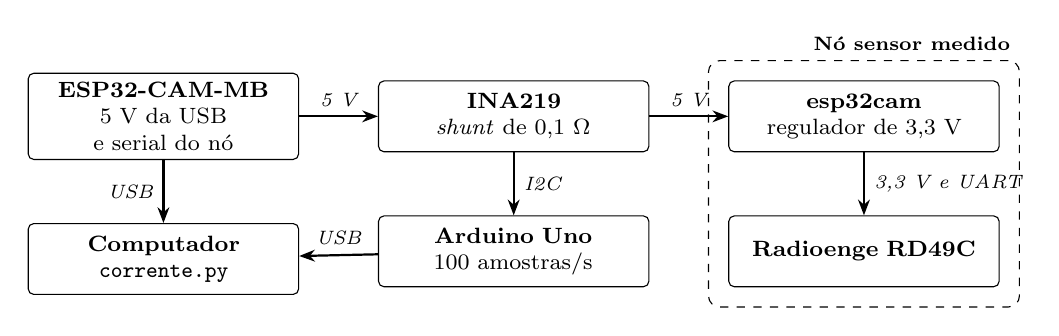
\begin{tikzpicture}[
        font=\footnotesize,
        node distance=8mm and 10mm,
        bloco/.style={draw, rounded corners=2pt, align=center, fill=white,
                      minimum height=9mm, text width=#1},
        bloco/.default=3.2cm,
        seta/.style={-{Stealth[length=2mm]}, thick},
        rotulo/.style={font=\scriptsize\itshape, align=center}
    ]
        \node[bloco] (mb) {\textbf{ESP32-CAM-MB}\\5~V da USB e serial do nó};
        \node[bloco, right=of mb] (ina) {\textbf{INA219}\\\textit{shunt} de 0,1~$\Omega$};
        \node[bloco, right=of ina] (cam) {\textbf{\gls{esp32cam}}\\regulador de 3,3~V};
        \node[bloco, below=of cam] (radio) {\textbf{Radioenge RD49C}};
        \node[bloco, below=of ina] (uno) {\textbf{Arduino Uno}\\100 amostras/s};
        \node[bloco, below=of mb] (pc) {\textbf{Computador}\\\texttt{corrente.py}};
        \node[draw, dashed, rounded corners=4pt, inner sep=2.5mm, fit=(cam) (radio),
              label={[font=\scriptsize\bfseries, anchor=south east]north east:Nó sensor medido}] {};

        \draw[seta] (mb) -- node[rotulo, above] {5~V} (ina);
        \draw[seta] (ina) -- node[rotulo, above] {5~V} (cam);
        \draw[seta] (cam) -- node[rotulo, right] {3,3~V e UART} (radio);
        \draw[seta] (ina) -- node[rotulo, right] {I2C} (uno);
        \draw[seta] (uno) -- node[rotulo, above] {USB} (pc);
        \draw[seta] (mb) -- node[rotulo, left] {USB} (pc);
    \end{tikzpicture}
    \legend{Fonte: Elaborado pelos autores (2026).}
\end{figure}

O INA219 foi configurado com o ganho que admite até 320~mV no resistor (3,2~A), para não
saturar nos picos de transmissão. A corrente é calculada no computador pela tensão no
resistor, cujo passo de 10~µV corresponde a 0,1~mA. Com o nó desconectado, a leitura foi de
0,00~mV, de modo que nenhum \textit{offset} foi descontado. Considerando a tolerância do
resistor e o \textit{offset} típico do sensor, a incerteza é de cerca de 1~mA mais 1\% da
leitura, o que torna confiáveis apenas as correntes de repouso acima de alguns
miliampères. A taxa de 100 amostras por segundo registra cerca de 13 amostras em cada
pacote de 135,8~ms no ar.

A análise, feita pelo \textit{script} \texttt{corrente.py}, separa os ciclos pelos trechos
de repouso. O nível de repouso é estimado pela mediana dos 10\% menores valores da
captura, e todo trecho abaixo de um limiar, de 5~mA ou 50\% acima desse nível, o que for
maior, com pelo menos 12~s de duração, é considerado repouso. Cada ciclo vai do fim de um
repouso ao fim do seguinte, e a carga do ciclo é calculada pela
Equação~\eqref{eq:carga_leitura}. A duração mínima de 12~s foi necessária porque picos
isolados de uma única amostra, de cerca de 61~mA, partiam alguns trechos de repouso em
dois e criavam ciclos falsos. Foram feitas duas capturas principais:

\begin{itemize}
    \item \textbf{Fluxo em nuvem}: 685.000 amostras em 6.850~s, a partir das 9h29. Dos 31
    ciclos encontrados, um foi excluído: o mesmo despertar sem envio excluído na medição de
    latência, em que o nó ficou acordado por 0,97~s. Restaram 30 ciclos completos.
    \item \textbf{Fluxo em borda}: 169.738 amostras em 1.697~s, das 12h22 às 12h49, com 32
    ciclos completos.
\end{itemize}

Antes dessas capturas, um teste curto de quatro ciclos com uma versão anterior do firmware
do fluxo em nuvem, que mantinha a câmera ligada durante todo o envio, foi usado como
referência para medir o efeito de desligá-la após a captura.

A partir das médias medidas de corrente e tempo acordado de cada fluxo, a autonomia foi
estimada pela Equação~\eqref{eq:autonomia_modelo} para uma bateria hipotética de
2.000~mAh e para intervalos de 10~minutos e de 1~hora entre leituras. A corrente de
repouso medida, de cerca de 24~mA, inclui o Radioenge, que permanece ligado durante o
\textit{deep sleep} do ESP32 (Seção~\ref{subsubsec:ciclo_operacao}), e os demais
componentes da placa. A medição que separaria essas parcelas, com o módulo desconectado,
não foi realizada. Por isso, a estimativa foi repetida com correntes de repouso hipotéticas
de 5, 1 e 0,1~mA, para mostrar como o resultado depende desse valor.


\section{Resultados e análises}
\label{sec:resultados}
% Cores dos gráficos: a mesma cor identifica o mesmo fluxo em todas as figuras
\definecolor{corNuvem}{HTML}{2A78D6}
\definecolor{corBorda}{HTML}{EB6834}
\definecolor{corFatias}{HTML}{008300}
\definecolor{corVotacao}{HTML}{6250D6}
\definecolor{corGrade}{HTML}{E1E0D9}
\definecolor{corEixo}{HTML}{898781}
\pgfplotsset{
    estiloResultados/.style={
        grid=major, grid style={color=corGrade, line width=0.3pt},
        axis x line*=bottom, axis y line*=left,
        axis line style={color=corEixo}, tick style={color=corEixo},
        tick label style={font=\scriptsize}, label style={font=\footnotesize},
        title style={font=\footnotesize},
        legend style={font=\scriptsize, draw=none, fill=white, fill opacity=0.85,
                      text opacity=1},
        legend cell align=left,
        /pgf/number format/use comma, /pgf/number format/1000 sep={.},
    },
}

Esta seção apresenta os resultados dos experimentos descritos na
Seção~\ref{sec:experimentos} e os analisa à luz das hipóteses da
Seção~\ref{subsec:hipotese}. Salvo indicação em contrário, os valores foram calculados a
partir dos dados brutos versionados no repositório do projeto, com os \textit{scripts} de
análise descritos naquela seção. A Seção~\ref{subsec:sintese_resultados} reúne o resultado
de cada hipótese, e a Seção~\ref{subsec:limitacoes_resultados}, as limitações que devem
acompanhar a sua leitura.

\subsection{Reconhecimento dos dígitos e efeito da quantização (H1)}
\label{subsec:resultado_h1}

A Tabela~\ref{tab:resultado_quantizacao} apresenta o desempenho do classificador de
dígitos. Nos 7.378 recortes de validação, o modelo em ponto flutuante acertou 7.043
(95,46\%) e o modelo em INT8, 7.037 (95,38\%): a quantização custou seis recortes, ou
0,08 ponto percentual.

\begin{table}[H]
    \centering
    \caption{Desempenho do classificador de dígitos em ponto flutuante e em INT8}
    \label{tab:resultado_quantizacao}
    \begin{tabularx}{\textwidth}{@{}>{\raggedright\arraybackslash}Xlrrr@{}}
        \toprule
        \textbf{Conjunto} & \textbf{Modelo} & \textbf{Leitura exata} & \textbf{Acerto por dígito} & \textbf{CER} \\
        \midrule
        Validação (7.378 recortes) & Ponto flutuante & --- & 95,46\% & --- \\
                                   & INT8            & --- & 95,38\% & --- \\
        \addlinespace
        Teste independente \textit{Word-Wheel} & INT8, fase A & 92,4\% & 97,3\% & 0,026 \\
        (1.894 imagens, 9.719 dígitos)          & INT8, fases A e B & 92,8\% & 97,7\% & 0,023 \\
        \bottomrule
    \end{tabularx}
    \legend{Fonte: Elaborado pelos autores (2026). Na validação, cada recorte é um único
    dígito, de modo que a acurácia por recorte coincide com o acerto por dígito.}
\end{table}

Como os dois modelos foram avaliados sobre os mesmos recortes, a comparação foi feita de
forma pareada. As duas versões deram a mesma resposta em 99,62\% dos recortes. Dos que
divergiram, 14 foram acertados apenas pelo modelo em ponto flutuante e 8 apenas pelo modelo
INT8. Pelo teste exato de McNemar, que considera apenas esses pares discordantes, a
diferença não é estatisticamente significativa ($p = 0{,}29$). A ordem de grandeza da perda
também aparece em outro detalhe: executado com os \textit{kernels} otimizados XNNPACK, em
vez dos \textit{kernels} sem esse delegado usados no restante do trabalho, o mesmo arquivo
INT8 acertou 7.040 recortes. A troca da implementação dos operadores altera o resultado na
mesma escala que a própria quantização.

O resultado é coerente com o tamanho e a forma do modelo. A quantização completa após o
treinamento, calibrada com um conjunto representativo, foi suficiente para um classificador
convolucional pequeno, com ativações ReLU, e o pipeline B não precisou do treinamento
consciente da quantização descrito na Seção~\ref{sec:fundamentos}, que no pipeline A havia
sido usado justamente para mitigar a degradação \cite{ferreira2022compressao}. Os dois
modelos INT8 somam 93,3~KB (81,5~KB do classificador e 11,8~KB da localização), na faixa de
centenas de quilobytes relatada para modelos de \gls{ocr} de medidores em hardware
embarcado \cite{ademola2023resource, jawas2018water}.

Por classe, a acurácia em INT8 variou de 90,84\% no dígito 7 a 97,21\% no dígito 0, que é
também o mais frequente. Os dígitos 7, 9 e 6 foram os mais difíceis (90,84\%, 91,64\% e
92,18\%). Dos 341 erros, 110 (32\%) foram classificações como 0, o que indica que os pesos
por classe compensaram apenas em parte o excesso de zeros no treino.

No teste independente, com as 1.894 imagens que ficaram fora de todo o treinamento, o
modelo INT8 leu 92,8\% das leituras inteiras e 97,7\% dos dígitos, com CER de 0,023. O
ajuste fino com as imagens do \gls{esp32cam} (fase B) não prejudicou a generalização:
melhorou 0,4 ponto percentual a leitura exata em relação ao modelo da fase A. Esse número
é inferior aos 95,6\% de leituras exatas que uma versão anterior do classificador obtinha
nesse mesmo conjunto, mas aquela versão havia sido treinada com essas imagens. A diferença
mostra o quanto um teste contaminado pelo treino superestima o desempenho, e é por isso que
o valor adotado é o do teste independente.

Quanto à hipótese H1, o modelo INT8 teve, de fato, acurácia menor que a do modelo em ponto
flutuante, como previsto. A redução, porém, é de 0,08 ponto percentual e não é
estatisticamente significativa, de modo que, na prática, a quantização não penalizou o
reconhecimento. Além disso, como os dois fluxos executam os mesmos modelos INT8
(Seção~\ref{subsec:visao_geral}), a acurácia não é um fator de diferença entre eles: o
servidor poderia executar o modelo em ponto flutuante sem restrição de memória, mas
ganharia no máximo essa mesma fração.

\subsection{Leitura de ponta a ponta}
\label{subsec:resultado_leitura}

A Tabela~\ref{tab:resultado_leitura} apresenta a leitura completa, da imagem da câmera até a
sequência de dígitos, nas configurações descritas na Seção~\ref{subsubsec:exp_leitura}.

\begin{table}[H]
    \centering
    \caption{Leitura de ponta a ponta nos dois fluxos}
    \label{tab:resultado_leitura}
    \begin{tabularx}{\textwidth}{@{}>{\raggedright\arraybackslash}X>{\raggedright\arraybackslash}p{3.4cm}rrrr@{}}
        \toprule
        & & \multicolumn{2}{c}{\textbf{Fluxo em borda}} & \multicolumn{2}{c}{\textbf{Fluxo em nuvem}} \\
        \cmidrule(lr){3-4}\cmidrule(l){5-6}
        \textbf{Conjunto} & \textbf{Janela de dígitos} & \textbf{Leituras} & \textbf{Dígitos} & \textbf{Leituras} & \textbf{Dígitos} \\
        \midrule
        \multirow{3}{=}{Comum (39 fotos, 222 dígitos)}
                         & Prevista pelo modelo & 0\% & 15\% & 0\% & 16\% \\
                         & Marcada à mão        & 46\% & 85\% & 46\% & 85\% \\
                         & Marcada à mão, quadro endireitado & --- & --- & 82\% & 92\% \\
        \addlinespace
        \multirow{3}{=}{Físico (21 fotos, 152 dígitos)}
                         & Prevista pelo modelo & 10\% & 31\% & 0\% & 27\% \\
                         & Marcada à mão, quadro endireitado & 10\% & 36\% & 10\% & 37\% \\
                         & Marcada à mão, endireitado, tons invertidos no fundo escuro & 14\% & 56\% & 14\% & 56\% \\
        \bottomrule
    \end{tabularx}
    \legend{Fonte: Elaborado pelos autores (2026). Leituras: taxa de leitura exata;
    dígitos: acerto por dígito. No conjunto comum, a inclinação é estimada pela transformada
    de Hough e só é corrigida no servidor; no físico, é marcada à mão e corrigida nos dois
    fluxos.}
\end{table}

\subsubsection{O gargalo é a localização da janela}

Com a janela prevista pelo modelo de localização, nenhuma das 39 fotos do conjunto comum
foi lida corretamente, em nenhum dos dois fluxos, e apenas 15\% a 16\% dos dígitos
coincidiram com o gabarito. Esse resultado
\textbf{não mede o classificador}. Nesse conjunto, a máscara prevista teve Dice de 0,23 e
IoU de 0,13 em relação à janela real, valores ainda menores que os do teste do próprio
modelo (Seção~\ref{subsubsec:segmentacao}), e a caixa prevista teve mediana de
$130 \times 90$ pixels, contra cerca de $97 \times 18$ pixels da janela real. Com uma caixa
que cobre quase todo o mostrador, as fatias não correspondem aos roletes. Endireitar o
quadro no servidor antes da localização também não resolveu: a caixa continuou com cerca de
90 pixels de altura, e a leitura exata continuou em 0\%.

Quando a janela é marcada à mão, o mesmo classificador, com o mesmo fatiamento, leu 46\%
das leituras e 85\% dos dígitos; com o quadro endireitado pelo servidor, chegou a 82\% das
leituras e 92\% dos dígitos. No medidor de seis roletes, com 27 fotos, foram 85\% das
leituras e 97\% dos dígitos. A diferença entre 0\% e 82\% vem inteiramente da janela: o
modelo de reconhecimento é o mesmo nas duas linhas. As sete leituras que ainda falharam
nessa configuração são as três fotos de uma mesma leitura com contraste muito baixo e
quatro fotos de duas leituras do medidor de seis roletes, cada uma com um ou dois dígitos
trocados.

Esse comportamento se repetiu no hardware. Nas primeiras capturas do firmware de
depuração, antes do ajuste da posição da câmera, a caixa prevista era enorme e a leitura,
errada.
Depois que a câmera foi posicionada à mão, de modo que a janela ocupasse a maior parte do
quadro, a caixa encolheu, e as doze últimas capturas leram a leitura real do medidor de
teste, \texttt{046663}. Nas cinco capturas do \gls{esp32cam} com a janela marcada à mão
(Figura~\ref{fig:leitura_caixa_manual}), todas as leituras e os 26 dígitos foram
reconhecidos.

\subsubsection{A compressão JPEG não afeta a leitura}

Com a janela marcada à mão, os dois fluxos tiveram exatamente o mesmo número de leituras
exatas (18 de 39) e de dígitos corretos (189 de 222). A compressão JPEG com qualidade 90,
que o fluxo em nuvem aplica antes da transmissão, não alterou a leitura. Com a janela
prevista pelo modelo, por outro lado, os dois fluxos deram a mesma leitura em apenas 10 das
39 fotos: pequenas diferenças introduzidas pela compressão mudam a máscara prevista e, com
ela, a caixa. A compressão afeta o modelo de localização, que já falha, e não o
classificador.

\subsubsection{Precisão exigida da ROI}

Como a solução adotada substitui a localização automática por uma ROI calibrada na
instalação, a Figura~\ref{fig:tolerancia_roi} mostra quanto erro de posição a leitura
tolera. Sem erro, a leitura exata é de 82\% com fatias iguais e de 87\% com a votação entre
cinco caixas deslocadas. Com até 2~pixels de erro em cada coordenada, cai para 62\% e 70\%;
com até 6~pixels, para 20\% e 26\%. Como cada dígito tem cerca de 16~pixels de largura no
quadro de $160 \times 120$ pixels, um erro de 2~pixels já corresponde a um oitavo de dígito.
A votação compensa cerca de 1~pixel de erro: com ela, a leitura com $\pm$2~pixels fica
próxima da leitura sem votação com $\pm$1~pixel. O custo é executar o classificador cinco
vezes.

\begin{figure}[H]
    \centering
    \caption{Leitura exata em função do erro de posição da ROI}
    \label{fig:tolerancia_roi}
    \begin{tikzpicture}
        \begin{axis}[
            estiloResultados,
            width=0.82\textwidth, height=6.2cm,
            xmin=-0.3, xmax=6.3, ymin=0, ymax=100,
            xtick={0,1,2,3,4,6}, xticklabels={0,$\pm$1,$\pm$2,$\pm$3,$\pm$4,$\pm$6},
            ytick={0,20,40,60,80,100},
            xlabel={Erro máximo sorteado em cada coordenada da ROI (pixels)},
            ylabel={Leituras exatas (\%)},
            legend pos=south west,
        ]
            \addplot[color=corFatias, line width=1pt, mark=*, mark size=1.8pt]
                coordinates {(0,82) (1,71) (2,62) (3,51) (4,40) (6,20)};
            \addlegendentry{Fatias iguais}
            \addplot[color=corVotacao, line width=1pt, mark=square*, mark size=1.7pt,
                     densely dashed, mark options={solid}]
                coordinates {(0,87) (1,81) (2,70) (3,64) (4,50) (6,26)};
            \addlegendentry{Votação entre 5 caixas}
            \node[font=\scriptsize, color=black, anchor=west] at (axis cs:0.1,91) {87\%};
            \node[font=\scriptsize, color=black, anchor=north west] at (axis cs:0.05,80) {82\%};
            \node[font=\scriptsize, color=black, anchor=south] at (axis cs:2,72) {70\%};
            \node[font=\scriptsize, color=black, anchor=north] at (axis cs:2,59) {62\%};
        \end{axis}
    \end{tikzpicture}
    \legend{Fonte: Elaborado pelos autores (2026). Conjunto comum, fluxo em nuvem, quadro
    endireitado; média de três sorteios do erro.}
\end{figure}

Calibrar a ROI com uma única leitura e aplicá-la às demais fotos do mesmo medidor rendeu
apenas 26\% a 30\% das leituras no medidor de seis roletes e 0\% no de cinco. Esse cenário,
porém, é pessimista: as fotos do conjunto comum são de um monitor cujo zoom e cuja posição
mudaram entre leituras, o que deslocou a janela em 3,5 a 5~pixels, em média, no primeiro
medidor e em 12 a 18~pixels no segundo. Os valores confirmam que a precisão da calibração é
o fator que decide a leitura: em uma instalação com a câmera fixada mecanicamente, espera-se
que a janela não se desloque entre leituras, mas essa condição não foi testada.

\subsubsection{Hidrômetros físicos}

No conjunto de hidrômetros físicos, com a janela prevista pelo modelo, o fluxo em borda
leu 2 das 21 fotos e o fluxo em nuvem, nenhuma, com 27\% a 31\% dos dígitos corretos. As
duas leituras corretas são de fotos em que a janela de dígitos ocupa a maior parte do
quadro, a mesma condição em que a caixa prevista se aproximou da janela no firmware de
depuração.

Com a janela e a inclinação marcadas à mão, porém, o resultado mudou pouco: 2 das 21
leituras e 36\% a 37\% dos dígitos, nos dois fluxos. Ao contrário do conjunto comum,
portanto, nos medidores reais a localização da janela não é a única causa dos erros. A
Tabela~\ref{tab:resultado_fisico_polaridade} separa as fotos pela polaridade da janela e
mostra de onde eles vêm.

\begin{table}[H]
    \centering
    \caption{Leitura do conjunto físico com a janela marcada à mão, por polaridade da janela}
    \label{tab:resultado_fisico_polaridade}
    \begin{tabularx}{\textwidth}{@{}>{\raggedright\arraybackslash}Xcrrrr@{}}
        \toprule
        & & \multicolumn{2}{c}{\textbf{Tons originais}} & \multicolumn{2}{c}{\textbf{Tons invertidos}} \\
        \cmidrule(lr){3-4}\cmidrule(l){5-6}
        \textbf{Fotos} & \textbf{Qtd.} & \textbf{Leituras} & \textbf{Dígitos} & \textbf{Leituras} & \textbf{Dígitos} \\
        \midrule
        Dígitos escuros em fundo claro, fotos frontais & 7 & 2 & 43/48 & --- & --- \\
        Dígitos escuros em fundo claro, perspectiva extrema & 2 & 0 & 2/10 & --- & --- \\
        Dígitos claros em fundo escuro & 12 & 0 & 11/94 & 1 & 40/94 \\
        \bottomrule
    \end{tabularx}
    \legend{Fonte: Elaborado pelos autores (2026). Fluxo em nuvem; leituras: número de
    leituras exatas. A inversão só se aplica às fotos de fundo escuro.}
\end{table}

Nas sete fotos frontais de medidores com dígitos escuros em fundo claro, o classificador
acertou 43 dos 48 dígitos (90\%), resultado próximo ao do conjunto comum, e duas fotos foram
lidas por inteiro; dos cinco dígitos errados, três estão no último rolete, parado entre dois
números. Nas duas fotos com perspectiva extrema, em que os dígitos aparecem inclinados em
relação às fatias, a leitura falhou.

Nas 12 fotos de medidores com dígitos claros em fundo escuro, o classificador respondeu 0
na maior parte das fatias e acertou apenas 11 dos 94 dígitos (12\%). A causa está no
treino: considerando de fundo escuro os recortes cuja mediana dos pixels fica abaixo de 100,
apenas 421 dos 49.038 recortes de treino (0,9\%) têm essa polaridade, e o modelo responde
com a classe mais frequente. Invertendo os tons da janela nessas fotos, o que equivale a
informar a polaridade do medidor na instalação, assim como o número de roletes, o acerto
subiu para 40 dos 94 dígitos (43\%), e uma foto passou a ser lida por inteiro. As fotos que
continuaram com erros têm perspectiva forte, reflexos no vidro, baixo contraste, dígitos com
cerca de 10 pixels de largura ou a janela cortada pela borda do quadro. A votação entre
caixas deslocadas não melhorou o resultado.

Com a janela, a inclinação e a polaridade informadas, o conjunto físico chegou a 3 das 21
leituras (14\%) e 56\% dos dígitos. Os erros que restam, porém, não têm todos a mesma
origem, e a maior parte não está no fluxo nem na janela. A
Tabela~\ref{tab:causas_erros_fisico} classifica as fotos pela causa dos erros.

\begin{table}[H]
    \centering
    \caption{Causas dos erros de leitura no conjunto físico}
    \label{tab:causas_erros_fisico}
    \begin{tabularx}{\textwidth}{@{}l>{\raggedright\arraybackslash}X>{\raggedright\arraybackslash}p{4.2cm}@{}}
        \toprule
        \textbf{Origem} & \textbf{Causa} & \textbf{Fotos} \\
        \midrule
        Captura & Perspectiva extrema, com os dígitos inclinados em relação às fatias & 01, 06, 11, 21, 26 \\
        Captura & Janela cortada pela borda do quadro & 21, 23, 25 \\
        Captura & Reflexo no vidro, baixo contraste ou dígitos com cerca de 10 pixels de largura & 02, 05, 15, 16 \\
        \addlinespace
        Treino & Dígitos claros em fundo escuro & 02, 03, 05, 06, 07, 11, 13, 15, 16, 21, 23, 24 \\
        Treino & Último rolete parado entre dois números & 04, 20, 25 \\
        \addlinespace
        Classificador & Dígito visível lido como 0 & 08, 22 \\
        \bottomrule
    \end{tabularx}
    \legend{Fonte: Elaborado pelos autores (2026). Uma foto pode ter mais de uma causa. As
    fotos 12 e 19 foram lidas sem erro com a janela marcada à mão.}
\end{table}

As causas de captura são resolvidas por uma instalação adequada, com a câmera de frente para
o medidor e a janela inteira no quadro, e não indicam falha do \gls{ocr}. As causas de
treino, ao contrário, são limitações do classificador, e não das fotos. A foto 07, por
exemplo, é frontal e nítida, mas foi lida como \texttt{00000000} com os tons originais e por
inteiro com os tons invertidos. O rolete parado entre dois números, por sua vez, ocorre em
qualquer medidor em uso, mas as imagens com essa situação foram descartadas do principal
conjunto de treino por terem rótulo ambíguo (Seção~\ref{subsubsec:dados_ocr}). Restam, por
fim, erros do próprio classificador em dígitos visíveis, raros nas fotos de boa qualidade.

Para estimar o desempenho em uma instalação adequada, foram separadas as fotos que atendem a
três condições: câmera frontal, sem perspectiva extrema; dígitos escuros em fundo claro, a
polaridade do treino; e todos os dígitos visíveis no quadro. Restaram seis fotos (04, 08,
12, 19, 20 e 22), com 41 dígitos. Com a janela marcada à mão, o classificador acertou 37 dos
41 dígitos (90,2\%, com intervalo de confiança de 95\% de 77,5\% a 96,1\%) e leu por
inteiro duas das seis fotos, nos dois fluxos; com a janela prevista pelo modelo, o acerto foi
de 61\% a 66\% dos dígitos. Dos quatro dígitos errados, dois estão no último rolete, parado
entre dois números, e dois são dígitos visíveis lidos como 0. Esse subconjunto foi definido
depois da avaliação do conjunto completo e é pequeno, de modo que deve ser lido como uma
indicação do que uma instalação adequada permite, e não como substituto do resultado das 21
fotos.

Os resultados do conjunto físico indicam, portanto, o que uma instalação real precisa:
câmera frontal com a janela inteira no quadro; ROI, inclinação e polaridade calibradas; e um
classificador treinado também com dígitos claros em fundo escuro, por exemplo pela inversão
dos recortes no aumento de dados, e com roletes em transição.

Em síntese, os resultados próximos de zero obtidos com a janela prevista pelo modelo são
causados pela localização automática, e não pelo classificador nem pelo fluxo: com a janela
informada, a leitura chega a 82\% das leituras e 92\% dos dígitos no conjunto comum e a
90\% dos dígitos nas fotos de medidores reais que atendem às condições de instalação, e o
classificador reconhece 97,7\% dos dígitos de um conjunto público independente. Em
medidores reais, porém, a janela correta não basta: a geometria da captura, que a instalação
resolve, e as limitações do treino quanto à polaridade e aos roletes em transição também
limitam a leitura. Como os dois fluxos executam o mesmo pipeline e a compressão não altera a
leitura, essas conclusões valem igualmente para a borda e para a nuvem.

\subsection{Latência (H2)}
\label{subsec:resultado_latencia}

A Tabela~\ref{tab:resultado_latencia} apresenta a latência ponta a ponta dos dois fluxos,
medida com o nó no modo autônomo.

\begin{table}[H]
    \centering
    \caption{Latência ponta a ponta dos dois fluxos}
    \label{tab:resultado_latencia}
    \begin{tabularx}{\textwidth}{@{}Xrr@{}}
        \toprule
        \textbf{Marco, desde o disparo} & \textbf{Fluxo em nuvem} & \textbf{Fluxo em borda} \\
        \midrule
        Captura concluída & 0,70~s & --- \\
        Leitura pronta no nó & --- & 18,20~s \\
        Primeiro pacote no computador & 1,97~s & 18,84~s \\
        \textbf{Dado disponível no servidor (mediana)} & \textbf{189,1~s} & \textbf{18,84~s} \\
        Mínimo e máximo & 172,7 a 213,5~s & 18,836 a 18,840~s \\
        Desvio-padrão & 11,8~s & 0,9~ms \\
        Leituras consideradas & 20 imagens completas & 27 leituras recebidas \\
        \bottomrule
    \end{tabularx}
    \legend{Fonte: Elaborado pelos autores (2026).}
\end{table}

A latência do fluxo em borda foi de 18,84~s, cerca de dez vezes menor que os 189,1~s do
fluxo em nuvem. Na corrida controlada, com o nó sempre ligado, a latência do fluxo em nuvem
foi de 197,1~s (de 148,1 a 204,9~s, com 21 imagens completas), compatível com a corrida em
modo autônomo, já que as imagens dessa corrida foram maiores (mediana de 4.379 contra
4.068~bytes).

Os dois fluxos têm gargalos opostos. No fluxo em nuvem, a imagem fica pronta em 0,70~s, e
quase toda a latência é a transmissão. Cada bloco leva cerca de 8,1~s: os 7~s do intervalo
entre pacotes e cerca de 1,1~s de comando AT, transmissão e confirmação do módulo. Por isso,
a latência cresce com o tamanho do JPEG: as três imagens mais rápidas tinham 22 blocos e
chegaram em cerca de 173~s, e a mais lenta, com 27 blocos, em 213,5~s. O tempo no ar
propriamente dito, de cerca de 3~s por imagem (Tabela~\ref{tab:tempo_no_ar}), representa
menos de 2\% da latência. Em 3 das 30 leituras, o primeiro bloco só chegou entre 10 e 12~s
após o disparo, o que indica que o bloco inicial se perdeu. A execução do \gls{ocr} no servidor, que
não está incluída na medição, leva cerca de 6~ms (Tabela~\ref{tab:tempo_inferencia}) e não
altera esses números.

No fluxo em borda, ao contrário, quase toda a latência é processamento. A leitura fica
pronta no nó em 18,20~s, dos quais cerca de 15,5~s são a localização da janela e 2,0~s a
classificação dos dígitos, segundo o log do próprio firmware; o envio e a recepção levam
mais 0,64~s. Como nenhum desses passos depende da rede, a latência é praticamente
determinística, com desvio-padrão de 0,9~ms.

Dois cenários ajudam a avaliar se a conclusão depende das escolhas de implementação. Ambos
são estimativas, e não medições. No fluxo em borda, retirar a localização da janela, como
prevê a solução com ROI calibrada, reduziria a latência para cerca de 3,3~s. No fluxo em
nuvem, mesmo eliminando o intervalo de 7~s entre pacotes, que é uma escolha conservadora e
não uma exigência regulatória (Seção~\ref{subsubsec:formato_mensagens}), restaria cerca de
1,1~s por bloco, ou aproximadamente 26~s para uma imagem de 24 blocos, acima da latência
medida no fluxo em borda. Assim, a vantagem do processamento local em latência não depende
do intervalo escolhido.

Quanto à latência, a hipótese H2 foi confirmada com folga, em concordância com a menor
latência atribuída à computação em borda na
Tabela~\ref{tab:vant_desvant_edge_cloud} \cite{andriulo2024edge}. Nesta implementação, a
vantagem vem da quantidade de dados transmitida, e não da velocidade do processamento: o
microcontrolador é cerca de 2.800 vezes mais lento que o servidor na inferência, mas o
fluxo em borda transmite 9~bytes por leitura, contra cerca de 4~KB do fluxo em nuvem.

\subsection{Entrega dos dados (H2)}
\label{subsec:resultado_entrega}

A Tabela~\ref{tab:resultado_entrega} apresenta a entrega dos dados nas três corridas, por
pacote e por leitura.

\begin{table}[H]
    \centering
    \caption{Entrega por pacote e por leitura}
    \label{tab:resultado_entrega}
    \begin{tabularx}{\textwidth}{@{}Xrr@{}}
        \toprule
        \textbf{Corrida} & \textbf{\gls{pdr} por pacote} & \textbf{Entrega por leitura} \\
        \midrule
        Fluxo em nuvem, modo autônomo & 699/713 (98,0\%) & 20/30 (66,7\%) \\
        Fluxo em nuvem, modo controlado & 749/759 (98,7\%) & 21/30 (70,0\%) \\
        Fluxo em borda, modo autônomo & 27/34 (79,4\%) & 27/34 (79,4\%) \\
        \bottomrule
    \end{tabularx}
    \legend{Fonte: Elaborado pelos autores (2026).}
\end{table}

As duas métricas apontam em sentidos opostos. Por pacote, o fluxo em nuvem entregou mais:
98,0\% contra 79,4\%, diferença estatisticamente significativa (teste exato de Fisher,
$p < 0{,}001$). Por leitura, o fluxo em borda entregou mais: 79,4\% contra 66,7\%; com 30 e
34 leituras, porém, essa diferença não é estatisticamente significativa ($p = 0{,}27$), nem
em relação à corrida controlada ($p = 0{,}40$).

No fluxo em nuvem, a diferença entre as duas métricas decorre da fragmentação. Como nenhum
dos firmwares retransmite blocos no modo autônomo, basta um bloco perdido para que a imagem
não seja remontada: as dez imagens incompletas da corrida em modo autônomo perderam apenas
um ou dois blocos cada. Se cada bloco fosse perdido de forma independente, com a taxa
observada, seriam esperadas 18,7 imagens completas em 30, e foram obtidas 20; na corrida
controlada, 21,5 esperadas e 21 obtidas. Ou seja, a probabilidade de uma imagem chegar
inteira é aproximadamente o \gls{pdr} elevado ao número de blocos, e uma taxa de 98\% por
pacote resulta em pouco mais de 60\% das imagens de 24 blocos. A retransmissão seletiva dos
blocos perdidos recuperaria essas leituras, mas com tempo no ar e energia adicionais, e não
foi implementada no modo autônomo.

No fluxo em borda, as perdas não se explicam pelo sinal: o RSSI ficou entre $-31$ e
$-27$~dBm, e, nos dois ciclos perdidos registrados no log do nó, o módulo aceitou o envio
sem falhas. As perdas também não se distribuíram de maneira uniforme no fluxo em nuvem. Na
corrida controlada, 6 dos 10 blocos perdidos foram o primeiro ou o último de uma imagem,
embora esses blocos sejam apenas 60 dos 759 enviados: uma taxa de perda de 10\% nas
extremidades de cada sequência, contra 0,57\% nos blocos do meio (teste exato de Fisher,
$p < 0{,}001$). O \textit{uplink} do fluxo em borda é, ao mesmo tempo, o primeiro e o último
da sua sequência, e a sua taxa de perda, de 20,6\%, não difere significativamente da taxa
das extremidades ($p = 0{,}21$). A causa não foi investigada; a coincidência sugere que as
perdas estão associadas ao início e ao fim de uma sequência de transmissões, no módulo ou no
receptor de canal único, e não ao enlace de rádio.

Quanto à entrega, portanto, a hipótese H2 não foi confirmada: o fluxo em borda entregou
mais leituras, mas sem significância estatística, e entregou uma fração menor de pacotes.
O resultado mostra ainda que a métrica de interesse da aplicação é a entrega por leitura, e
não o \gls{pdr}: um \gls{pdr} de 98\% por pacote resultou em um terço das imagens perdidas.
Em um cenário com retransmissão, a diferença de custo seria grande: o fluxo em borda
reenviaria um pacote de 9~bytes, enquanto o fluxo em nuvem precisaria reenviar os blocos
faltantes e manter o nó acordado durante a espera.

\subsection{Consumo de energia e autonomia (H3)}
\label{subsec:resultado_energia}

A Figura~\ref{fig:corrente_ciclos} mostra a corrente do nó durante um ciclo típico de cada
fluxo, e a Tabela~\ref{tab:resultado_energia} resume as medições.

\begin{figure}[H]
    \centering
    \caption{Corrente do nó sensor em um ciclo de leitura de cada fluxo}
    \label{fig:corrente_ciclos}
    \begin{tikzpicture}
        \begin{groupplot}[
            estiloResultados,
            group style={group size=1 by 2, vertical sep=13mm},
            width=\textwidth, height=5cm,
            xmin=0, xmax=225, ymin=0, ymax=250,
            ytick={0,50,100,150,200,250},
            ylabel={Corrente (mA)},
        ]
            \nextgroupplot[title={(a) Fluxo em nuvem: ciclo de 219~s e 4,65~mAh}]
            \addplot[color=corNuvem, line width=0.35pt] table {sections/dados/corrente_ciclo_nuvem.dat};
            \node[font=\scriptsize, anchor=south] at (axis cs:95,212) {picos de transmissão, um por bloco};
            \node[font=\scriptsize, anchor=north] at (axis cs:95,72) {espera entre blocos, $\approx$80~mA};
            \node[font=\scriptsize, anchor=south] at (axis cs:205,30) {repouso};

            \nextgroupplot[title={(b) Fluxo em borda: ciclo de 49~s e 0,82~mAh},
                           xlabel={Tempo desde o despertar (s)}]
            \addplot[color=corBorda, line width=0.35pt] table {sections/dados/corrente_ciclo_borda.dat};
            \draw[-{Stealth[length=1.5mm]}, color=black!70, line width=0.4pt] (axis cs:57,114) -- (axis cs:22,114);
            \node[font=\scriptsize, anchor=west] at (axis cs:58,114) {inferência, $\approx$114~mA};
            \node[font=\scriptsize, anchor=south west] at (axis cs:21,212) {\textit{uplink}};
            \node[font=\scriptsize, anchor=west] at (axis cs:52,25) {repouso, $\approx$25~mA};
        \end{groupplot}
    \end{tikzpicture}
    \legend{Fonte: Elaborado pelos autores (2026). Ciclos com carga próxima da mediana de
    cada corrida; envelope dos valores mínimo e máximo a cada 0,25~s das amostras de 100~Hz.}
\end{figure}

\begin{table}[H]
    \centering
    \caption{Consumo do nó sensor por ciclo de leitura, com repouso de 30~s}
    \label{tab:resultado_energia}
    \begin{tabularx}{\textwidth}{@{}Xrr@{}}
        \toprule
        \textbf{Grandeza} & \textbf{Fluxo em nuvem} & \textbf{Fluxo em borda} \\
        \midrule
        Ciclos medidos & 30 & 32 \\
        \textbf{Carga por leitura (média)} & \textbf{4,64~mAh} & \textbf{0,824~mAh} \\
        Desvio-padrão da carga & 0,24~mAh & 0,014~mAh \\
        Carga apenas do tempo acordado & 4,46~mAh & 0,62~mAh \\
        Tempo acordado & 189,9~s (173 a 219~s) & 19,45~s \\
        Corrente média acordado & 84,5~mA & 114~mA \\
        Picos de transmissão & 207 a 220~mA & 206 a 227~mA \\
        Corrente em repouso & 23,7~mA & 25,2~mA \\
        Período do ciclo & 218,5~s & 49,1~s \\
        \bottomrule
    \end{tabularx}
    \legend{Fonte: Elaborado pelos autores (2026). No fluxo em borda, tempo acordado e
    corrente acordado são medianas; três ciclos tiveram a fronteira deslocada por picos
    isolados de uma amostra.}
\end{table}

Uma leitura do fluxo em nuvem consumiu 4,64~mAh, contra 0,824~mAh do fluxo em borda: 5,6
vezes mais. Considerando apenas o tempo acordado, sem o repouso, a razão é de 7,2 vezes
(4,46 contra 0,62~mAh). A Figura~\ref{fig:corrente_ciclos} mostra a origem da diferença. No
fluxo em nuvem, o nó passa cerca de 190~s acordado, a maior parte em espera entre blocos,
com a CPU ligada a cerca de 80~mA; os picos de transmissão acima de 150~mA ocupam só 2,2\%
do tempo acordado e respondem por 4,9\% da carga acordado. O consumo é determinado,
portanto, pelo tempo acordado, que depende do número de blocos e do intervalo entre eles,
e não pela energia do rádio. Isso explica também a variação entre ciclos, de 4,26 a
5,24~mAh, que acompanha o tamanho de cada imagem. No fluxo em borda, a corrente é maior
durante a inferência, cerca de 114~mA, mas o ciclo é dez vezes mais curto.

O consumo do fluxo em nuvem também mostra o efeito de decisões de firmware. Na versão
anterior, que mantinha a câmera ligada durante o envio, a corrente acordado era de 162~mA e
a leitura custava 6,62~mAh. Desligar a câmera logo após a captura reduziu a corrente
acordado em 48\% e a carga por leitura em 30\%; a redução da carga foi menor porque as
imagens da corrida final foram maiores, o que aumentou o tempo acordado. No fluxo em borda, a localização da janela responde por cerca de 0,48~mAh
dos 0,62~mAh acordado, considerando 15,5~s a cerca de 112~mA. Com a ROI calibrada, a carga
acordado cairia para cerca de 0,13~mAh, uma estimativa ainda não medida.

\subsubsection{Autonomia}

Com repouso de 30~s, a corrente em repouso responde por apenas 4\% da carga de uma leitura
no fluxo em nuvem, mas por 25\% no fluxo em borda. Em intervalos mais longos, ela passa a
dominar os dois fluxos. Os cerca de 24~mA medidos em repouso, porém, não são uma
característica dos fluxos: incluem o módulo Radioenge, que permanece ligado sem receber o
comando de suspensão, e os demais componentes da placa. Segundo o fabricante, o módulo
consome 1,8~µA quando suspenso \cite{radioenge2022}, de modo que esse piso pode ser muito
reduzido. Como a medição que separaria essas parcelas não foi feita, a autonomia foi
estimada com o piso medido e com pisos hipotéticos, pela
Equação~\eqref{eq:autonomia_modelo}. O modelo reproduz as cargas medidas (4,65 e
0,825~mAh), e os resultados estão na Tabela~\ref{tab:resultado_autonomia} e na
Figura~\ref{fig:autonomia}.

\begin{table}[H]
    \centering
    \caption{Autonomia estimada para uma bateria de 2.000~mAh}
    \label{tab:resultado_autonomia}
    \begin{tabular}{@{}llrrr@{}}
        \toprule
        \textbf{Intervalo} & \textbf{Corrente em repouso} & \textbf{Nuvem} & \textbf{Borda} & \textbf{Borda / nuvem} \\
        \midrule
        10~min & 24~mA (medida) & 1,9 dia & 3,1 dias & 1,6 \\
               & 5~mA          & 2,8 dias & 9,8 dias & 3,5 \\
               & 1~mA          & 3,0 dias & 17,8 dias & 5,9 \\
               & 0,1~mA        & 3,1 dias & 21,9 dias & 7,0 \\
        \addlinespace
        1~h    & 24~mA (medida) & 3,1 dias & 3,4 dias & 1,1 \\
               & 5~mA          & 9,1 dias & 14,9 dias & 1,6 \\
               & 1~mA          & 15,4 dias & 51,7 dias & 3,4 \\
               & 0,1~mA        & 18,3 dias & 116,1 dias & 6,3 \\
        \bottomrule
    \end{tabular}
    \legend{Fonte: Elaborado pelos autores (2026). Modelo ideal, sem perdas do regulador
    nem autodescarga; apenas a corrente de 24~mA foi medida.}
\end{table}

\begin{figure}[H]
    \centering
    \caption{Autonomia estimada em função da corrente em repouso}
    \label{fig:autonomia}
    \begin{tikzpicture}[
        declare function={
            autonomia(\i,\a,\r,\T) = 83.3333*\T/(\i*\a + \r*(\T - \a));
        }]
        \begin{groupplot}[
            estiloResultados,
            group style={group size=3 by 1, horizontal sep=6mm, yticklabels at=edge left},
            width=0.37\textwidth, height=6cm,
            xmode=log, ymode=log,
            xmin=0.01, xmax=30, ymin=1, ymax=3000,
            xtick={0.01,0.1,1,10}, xticklabels={{0,01},{0,1},1,10},
            ytick={1,10,100,1000}, yticklabels={1,10,100,{1.000}},
            log basis x=10, log basis y=10,
        ]
            \nextgroupplot[title={Leitura a cada 10~min}, ylabel={Autonomia (dias)},
                           legend to name=legendaAutonomia, legend columns=3,
                           legend style={draw=none, font=\scriptsize, /tikz/every even column/.append style={column sep=4mm}}]
            \addplot[color=corNuvem, line width=1pt, domain=-2:1.4771, samples=60]
                ({10^x}, {autonomia(84.5,189.9,10^x,600)});
            \addlegendentry{Fluxo em nuvem}
            \addplot[color=corBorda, line width=1pt, densely dashed, domain=-2:1.4771, samples=60]
                ({10^x}, {autonomia(114.4,19.45,10^x,600)});
            \addlegendentry{Fluxo em borda}
            \addlegendimage{color=black!55, line width=0.5pt}
            \addlegendentry{Corrente em repouso medida (24~mA)}
            \draw[color=black!55, line width=0.5pt] (axis cs:24,1) -- (axis cs:24,3000);

            \nextgroupplot[title={Leitura a cada 1~h}, xlabel={Corrente em repouso (mA)}]
            \addplot[color=corNuvem, line width=1pt, domain=-2:1.4771, samples=60]
                ({10^x}, {autonomia(84.5,189.9,10^x,3600)});
            \addplot[color=corBorda, line width=1pt, densely dashed, domain=-2:1.4771, samples=60]
                ({10^x}, {autonomia(114.4,19.45,10^x,3600)});
            \draw[color=black!55, line width=0.5pt] (axis cs:24,1) -- (axis cs:24,3000);

            \nextgroupplot[title={Leitura a cada 24~h}]
            \addplot[color=corNuvem, line width=1pt, domain=-2:1.4771, samples=60]
                ({10^x}, {autonomia(84.5,189.9,10^x,86400)});
            \addplot[color=corBorda, line width=1pt, densely dashed, domain=-2:1.4771, samples=60]
                ({10^x}, {autonomia(114.4,19.45,10^x,86400)});
            \draw[color=black!55, line width=0.5pt] (axis cs:24,1) -- (axis cs:24,3000);
        \end{groupplot}
        \node[anchor=north] at ($(group c2r1.south)+(0,-11mm)$) {\pgfplotslegendfromname{legendaAutonomia}};
    \end{tikzpicture}
    \legend{Fonte: Elaborado pelos autores (2026). Bateria hipotética de 2.000~mAh, modelo
    da Equação~\eqref{eq:autonomia_modelo} com os valores medidos de corrente e tempo
    acordado de cada fluxo.}
\end{figure}

Com o piso medido, a vantagem do fluxo em borda na autonomia é pequena: 1,6 vez com
leituras a cada 10~minutos e 1,1 vez a cada hora, com autonomias de poucos dias nos dois
casos. À medida que o piso diminui, a razão se aproxima da razão entre as cargas acordado,
de 7,2 vezes: com 0,1~mA, o fluxo em borda alcança 21,9 dias com leituras a cada 10~minutos,
contra 3,1 dias do fluxo em nuvem. A Figura~\ref{fig:autonomia} mostra também o efeito do
intervalo: com leituras diárias, mesmo um piso de 0,1~mA consome mais que as próprias
leituras, e a razão cai para 2,3 vezes (663 contra 292 dias).

Quanto à hipótese H3, o fluxo em nuvem apresentou, de fato, maior consumo por leitura e,
portanto, autonomia inferior, de modo que a hipótese foi confirmada. A magnitude da
diferença na autonomia, porém, depende menos do fluxo do que da corrente em repouso e do
intervalo entre leituras: vai de praticamente nula, com o piso medido e leituras horárias ou
diárias, a cerca de sete vezes, com um piso baixo e leituras frequentes. Para um projeto
real, o resultado indica que reduzir a corrente em repouso, suspendendo o módulo de rádio e
os demais componentes da placa, é condição para que a escolha do fluxo faça diferença na
autonomia.

\subsection{Desempenho computacional e complexidade de desenvolvimento}
\label{subsec:resultado_complexidade}

A pergunta de pesquisa inclui, além da energia e da acurácia, o desempenho computacional e
a complexidade de desenvolvimento do firmware, aspectos avaliados a partir das medições do
firmware e do servidor (Seções~\ref{subsec:firmware} e \ref{subsec:servidor}) e da
experiência de implementação.

Em desempenho computacional, a diferença é de mais de três ordens de grandeza: a leitura
completa levou 17.838~ms no \gls{esp32cam} e cerca de 6~ms no servidor
(Tabela~\ref{tab:tempo_inferencia}). A literatura relata inferência abaixo de um segundo
para modelos de \gls{ocr} de medidores em hardware embarcado
\cite{ademola2023resource, jawas2018water}; aqui, apenas a classificação dos seis dígitos
ficou próxima disso, com cerca de 330~ms por dígito, enquanto a localização da janela levou
15,6~s. A causa não foi investigada (Seção~\ref{subsubsec:tflm}). Ao contrário do
observado por \citeonline{bravo2025ants}, para quem medidores mais antigos ou obstruídos
podem elevar o tempo de processamento, o tempo de inferência aqui não depende do conteúdo
da imagem: variou apenas 4~ms em 61 capturas, pois a rede executa sempre as mesmas
operações.

A restrição de memória limitou a escolha dos modelos. O fluxo em borda reservou cerca de
2,9~MB da PSRAM para as \textit{arenas} e usou 1,65~MB (Tabela~\ref{tab:memoria_tflm}), e o
pipeline A foi descartado porque pedia uma \textit{arena} de
15,3~MB e um operador ausente na versão do TensorFlow Lite Micro disponível
(Seção~\ref{subsubsec:evolucao_ocr}). No servidor, nenhuma dessas restrições existe.

A complexidade de desenvolvimento também foi maior no fluxo em borda, ainda que os dois
firmwares tenham tamanhos parecidos, com 525 e 624 linhas. A diferença está fora do laço
principal. O fluxo em borda exigiu a quantização completa e a sua validação, a conversão
dos modelos em cabeçalhos C, o registro dos operadores de cada modelo, o dimensionamento das
\textit{arenas}, que falhou na primeira tentativa e motivou um \textit{script} de
estimativa, e um firmware de depuração para observar na placa o que o modelo via.
Recursos que melhoraram a leitura, como a correção de inclinação, que elevou a leitura exata
de 46\% para 82\%, e a votação entre caixas, foram implementados apenas no servidor. Por
fim, a manutenção também difere: atualizar o modelo no fluxo em nuvem significa trocar um
arquivo no servidor, enquanto no fluxo em borda exige regravar o firmware de cada nó, pois
a atualização remota não foi implementada. Essas observações confirmam, para este sistema,
a menor complexidade de firmware e a maior facilidade de manutenção atribuídas à computação
em nuvem, bem como a dificuldade de executar modelos de aprendizado de máquina na borda
(Tabela~\ref{tab:vant_desvant_edge_cloud}) \cite{andriulo2024edge}.

\subsection{Síntese e discussão}
\label{subsec:sintese_resultados}

A Tabela~\ref{tab:sintese_hipoteses} resume o resultado de cada hipótese.

\begin{table}[H]
    \centering
    \caption{Síntese dos resultados das hipóteses}
    \label{tab:sintese_hipoteses}
    \begin{tabularx}{\textwidth}{@{}l>{\raggedright\arraybackslash}X>{\raggedright\arraybackslash}p{3.6cm}@{}}
        \toprule
        \textbf{Hipótese} & \textbf{Resultado medido} & \textbf{Situação} \\
        \midrule
        H1 & INT8 com 95,38\% contra 95,46\% do modelo em ponto flutuante, diferença de 0,08
        ponto percentual sem significância estatística ($p = 0{,}29$) & Confirmada no sentido,
        mas a redução é desprezível \\
        \addlinespace
        H2, latência & 18,84~s no fluxo em borda contra 189,1~s no fluxo em nuvem & Confirmada \\
        \addlinespace
        H2, entrega & Por leitura, 79,4\% contra 66,7\%, sem significância ($p = 0{,}27$); por
        pacote, 79,4\% contra 98,0\% & Não confirmada \\
        \addlinespace
        H3 & 0,824 contra 4,64~mAh por leitura (5,6 vezes); autonomia de 1,0 a 7,0 vezes maior,
        conforme a corrente em repouso e o intervalo & Confirmada, com magnitude dependente
        do repouso \\
        \bottomrule
    \end{tabularx}
    \legend{Fonte: Elaborado pelos autores (2026).}
\end{table}

Em relação à pergunta de pesquisa, os resultados indicam que, em um enlace \gls{lorawan} de
baixa taxa, o volume de dados transmitido pesa mais do que a capacidade de processamento.
Mesmo com uma inferência cerca de 2.800 vezes mais lenta que a do servidor, o fluxo em borda
teve latência dez vezes menor e consumo por leitura de cinco a sete vezes menor, porque
transmite cerca de 450 vezes menos dados. A acurácia não diferenciou os fluxos: ambos
executam os mesmos modelos, a quantização teve efeito desprezível e a compressão JPEG não
alterou a leitura. O limite da acurácia, nos dois casos, está na localização da janela de
dígitos, que a calibração da ROI na instalação resolve quando a câmera é fixa, e, em
medidores reais, também na geometria da captura e no treino do classificador, que não cobre
dígitos claros em fundo escuro nem roletes em transição. O custo do
fluxo em borda aparece na complexidade de desenvolvimento e de manutenção e na restrição de
memória, que impede o uso de modelos maiores e de recursos como a correção de inclinação.

Em comparação com os trabalhos correlatos, \citeonline{bravo2025ants} relatam precisão de
99,71\% no reconhecimento dos dígitos com \gls{ocr} executado no próprio \gls{esp32cam}. O
classificador deste trabalho reconheceu 97,7\% dos dígitos em um conjunto público
independente e 92\% nas fotos do \gls{esp32cam} com a janela informada. Como os conjuntos de
dados são diferentes, os números não são diretamente comparáveis, mas os resultados aqui
obtidos indicam que, nesse tipo de sistema, a acurácia depende menos da arquitetura do
classificador do que de localizar corretamente a janela de dígitos e de o treino cobrir a
variedade dos medidores reais, como a polaridade dos dígitos. Em relação a \citeonline{SilvaVilela2021}, cujo trabalho não
apresentou métricas de consumo energético e de processamento, este trabalho quantifica essas
métricas para os dois métodos de processamento: carga por leitura, latência, tempo de
inferência e uso de memória.

\subsection{Limitações}
\label{subsec:limitacoes_resultados}

Os resultados devem ser interpretados considerando as seguintes limitações:

\begin{itemize}
    \item \textbf{Imagens de teste}: o conjunto comum, as fotos de ajuste fino e as de
    calibração foram capturadas de um monitor que exibia imagens de hidrômetros, sem os
    reflexos, a iluminação e os ângulos de um medidor instalado. O conjunto de hidrômetros
    físicos tem apenas 21 fotos, de medidores diferentes e não de uma instalação fixa, e as
    suas janelas, inclinações e polaridades foram marcadas pelos autores, sem conferência
    independente. O subconjunto que representa uma instalação adequada tem apenas seis fotos
    e foi definido após a avaliação do conjunto completo.
    \item \textbf{Acurácia emulada}: a acurácia dos dois fluxos foi medida por uma emulação
    em Python com os mesmos modelos. Na placa, as leituras não tinham gabarito; na corrida de
    latência do fluxo em borda, com a câmera fixa, as 27 leituras recebidas tiveram 13
    valores distintos, instabilidade que não foi investigada.
    \item \textbf{ROI não implementada no firmware}: o firmware medido ainda executa a
    localização da janela. Os valores de leitura em cerca de 2~s, latência de cerca de
    3,3~s e carga acordado de cerca de 0,13~mAh para a versão com ROI são estimativas.
    \item \textbf{Cenário de enlace}: as medições foram feitas em bancada, a 2~m de
    distância, com sinal forte, um receptor de canal único no lugar de um
    \textit{gateway} e sem retransmissão. As execuções em que o receptor ficou de 15 a 25
    minutos sem repassar quadros foram excluídas por se tratar de uma falha do receptor, cuja
    causa não foi identificada; a sua ocorrência indica que o receptor usado é um ponto
    frágil do protótipo. As amostras, de 30 a 34 leituras por fluxo, só permitem detectar
    diferenças grandes de entrega.
    \item \textbf{Energia}: a corrente em repouso inclui o módulo de rádio e os componentes
    da placa, e a medição que separaria essas parcelas não foi feita. O nó foi alimentado
    pela porta USB, e não pela bateria e pelo regulador de uma instalação real, e as
    autonomias vêm de um modelo ideal com bateria hipotética.
    \item \textbf{Instante de disparo}: o disparo foi marcado de 0,3 a 0,5~s após o
    despertar real, nos dois fluxos, e a latência do fluxo em nuvem não inclui a execução do
    \gls{ocr} no servidor, de cerca de 6~ms.
    \item \textbf{Escala}: os experimentos usaram um único nó, um único receptor e poucos
    medidores, de modo que não avaliam o comportamento de uma rede com vários dispositivos
    compartilhando o canal.
\end{itemize}


% ---------------------------------------------------------------
% CONCLUSÃO
% ---------------------------------------------------------------
\chapter{Conclusão}

\label{cap:conclusao}
% Capítulo a ser escrito.
\section{Retomada do problema e dos objetivos}
Retome o problema e destaque o que foi atingido.

\section{Contribuições para a Computação}
Explique o que a pesquisa trouxe de novo.

\section{Limitações e trabalhos futuros}
Liste limites e sugira próximos passos coerentes.

% ---------------------------------------------------------------
% OBSERVAÇÕES DO AUTOR
% ---------------------------------------------------------------
\chapter*{Observações importantes}
\addcontentsline{toc}{chapter}{Observações importantes}

Para graduação, Wazlawick aceita trabalhos aplicados desde que:
\begin{itemize}
    \item O problema seja preciso;
    \item A solução esteja fundamentada;
    \item Haja análise crítica;
    \item Não seja apenas entrega funcional.
\end{itemize}

% ---------------------------------------------------------------
% APRESENTAÇÃO ORAL (BANCA)
% ---------------------------------------------------------------
% \chapter*{Apresentação oral (banca)}
% \addcontentsline{toc}{chapter}{Apresentação oral (banca)}

% Além do documento escrito, o TCC2 é avaliado por uma \textbf{apresentação oral} final perante a banca. Um template pronto em \texttt{Beamer} está disponível no arquivo \texttt{apresentacao\_tcc2.tex}, na mesma pasta deste documento.

% \noindent\fbox{\parbox{\dimexpr\textwidth-2\fboxsep-2\fboxrule}{%
% \textbf{Regras da apresentação do TCC2}

% \vspace{0.2cm}
% \begin{itemize}
%     \item \textbf{Duração: 30 minutos.} Cronometre os ensaios; ultrapassar o tempo é penalizado. A arguição da banca ($\approx$ 5 min) ocorre após a apresentação, separada desse total.
%     \item \textbf{Cubra o trabalho completo}, seguindo a estrutura do documento escrito: introdução e problema, objetivos e método, desenvolvimento, \textbf{resultados e análise} e conclusão/contribuições.
%     \item \textbf{Dê peso aos resultados:} grande parte do tempo deve ser dedicada a apresentar e \textbf{analisar criticamente} os resultados, não apenas descrevê-los.
%     \item \textbf{Ritmo:} cerca de 1 a 1,5 minuto por slide, totalizando aproximadamente 20 a 26 slides de conteúdo.
%     \item \textbf{Logo do SENAC:} grande no primeiro slide (capa) e pequena no canto superior direito dos demais slides --- já configurado no template.
%     \item \textbf{Demonstração:} se houver demo ao vivo, tenha um plano B com capturas de tela ou vídeo curto.
%     \item \textbf{Slides de apoio (backup):} inclua slides extras após o ``Obrigado'' com detalhes técnicos, trechos de código e tabelas completas para a arguição.
% \end{itemize}

% \vspace{0.2cm}
% \textbf{Distribuição de tempo sugerida (30 min):} introdução/problema $\approx$ 4 min; objetivos/método $\approx$ 5 min; desenvolvimento $\approx$ 8 min; resultados/análise $\approx$ 8 min; conclusão $\approx$ 3 min; demonstração $\approx$ 2 min.
% }}

% ---------------------------------------------------------------
% ELEMENTOS PÓS-TEXTUAIS
% ---------------------------------------------------------------
\postextual

\pdfbookmark[0]{Glossário}{glossario}
\printglossary[type=main, title={Glossário}]

\bibliography{bibliografia_tcc2}

\end{document}
